% !Mode:: "TeX:UTF-8"
% !TEX encoding = UTF-8 Unicode

%----------------------------------------------------------------------------------------
% 机器翻译:统计建模与深度学习方法
% Machine Translation: Statistical Modeling and Deep Learning Methods
%
% Copyright 2020
% 肖桐(xiaotong@mail.neu.edu.cn) 朱靖波 (zhujingbo@mail.neu.edu.cn)
%----------------------------------------------------------------------------------------

%----------------------------------------------------------------------------------------
%    CONFIGURATIONS
%----------------------------------------------------------------------------------------

\renewcommand\figurename{图}%将figure改为图
\renewcommand\tablename{表}%将figure改为图
\chapterimage{fig-NEU-7.jpg} % Chapter heading image

%----------------------------------------------------------------------------------------
%	CHAPTER 7
%----------------------------------------------------------------------------------------

\chapter{基于短语的模型}

\parinterval 机器翻译的一个基本问题是要定义翻译的基本单元是什么。比如,可以像{\chapterfive}介绍的那样,以单词为单位进行翻译,即把句子的翻译看作是单词之间对应关系的一种组合。基于单词的模型是符合人类对翻译问题的认知的,因为单词本身就是人类加工语言的一种基本单元。然而,在进行翻译时也可以使用一些更“复杂”的知识。比如,很多词语间的搭配需要根据语境的变化进行调整,而且对于句子结构的翻译往往需要更上层的知识,如句法知识。因此,在对单词翻译进行建模的基础上,需要探索其他类型的翻译知识,使得搭配和结构翻译等问题可以更好地被建模。

\parinterval 本章会介绍基于短语的机器翻译模型。在过去二十年中,它一直是机器翻译的主流方法。相比于基于单词的模型,基于短语的模型可以更好地对单词之间搭配和小范围依赖关系进行描述。这种方法也在相当长的一段时期内占据着机器翻译的统治地位。即使近些年神经机器翻译逐渐崛起,基于短语的模型仍然是机器翻译的主要框架之一,其中的思想和很多技术手段对今天的机器翻译研究仍然有很好的借鉴意义。

%----------------------------------------------------------------------------------------
%    NEW SECTION
%----------------------------------------------------------------------------------------
\sectionnewpage
\section{翻译中的短语信息}

不难发现,基于单词的模型并不能很好地捕捉单词间的搭配关系。相比之下,使用更大颗粒度的翻译单元是一种对搭配进行处理的方法。下面来一起看看,基于单词的模型所产生的问题以及如何使用基于短语的模型来缓解该问题。

%----------------------------------------------------------------------------------------
%    NEW SUB-SECTION
%----------------------------------------------------------------------------------------

\subsection{词的翻译带来的问题}

\parinterval 首先,回顾一下基于单词的统计翻译模型是如何完成翻译的。图\ref{fig:7-1}展示了一个实例。其中,左侧是一个单词的“翻译表”,它记录了源语言(汉语)单词和目标语言(英语)单词之间的对应关系,以及这种对应的可能性大小(用$\funp{P}$表示)。在翻译时,会使用这些单词一级的对应,生成译文。图\ref{fig:7-1}右侧就展示了一个基于词的模型生成的翻译结果,其中$\seq{s}$和$\seq{t}$分别表示源语言和目标语言句子,单词之间的连线表示两个句子中单词一级的对应。

%----------------------------------------------
\begin{figure}[htp]
\centering
\begin{tabular}{l r}
\subfigure{%%%------------------------------------------------------------------------------------------------------------
%%% 基于单词的模型的问题


{\small
\begin{tabular}{l | l}
单词翻译表 & $\funp{P}$ \\ \hline
我 $\to$ I & 0.6 \\
喜欢 $\to$ like & 0.3 \\
绿 $\to$ green & 0.9 \\
茶 $\to$ tea & 0.8 \\
\end{tabular}
}

} & \subfigure{\begin{minipage}[c]{0.35\linewidth}
\begin{tikzpicture}

\begin{scope}
{\small
\node [anchor=west] (s1) at (0,0) {我};
\node [anchor=west] (s2) at ([xshift=1.0em]s1.east) {喜欢};
\node [anchor=west] (s3) at ([xshift=1.0em]s2.east) {{\color{ugreen} 绿}};
\node [anchor=west] (s4) at ([xshift=1.07em]s3.east) {茶};
\node [anchor=east] (s) at (s1.west) {$\seq{s}=$};
}
\end{scope}

{
\begin{scope}[yshift=-2.0em]
{\small
\node [anchor=west] (t1) at (0.35em,0) {I};
\node [anchor=west] (t2) at ([xshift=0.8em,yshift=-0.0em]t1.east) {like};
\node [anchor=west] (t3) at ([xshift=1.0em,yshift=-0.2em]t2.east) {green};
\node [anchor=west] (t4) at ([xshift=0.78em,yshift=0.1em]t3.east) {tea};
\node [anchor=east] (t) at ([xshift=-0.3em]t1.west) {$\seq{t}=$};
}
\end{scope}

\draw [-] (s1.south) -- (t1.north);
\draw [-] (s2.south) ..controls +(south:0.5em) and +(north:0.5em).. (t2.north);
\draw [-] (s3.south) ..controls +(south:0.5em) and +(north:0.5em).. (t3.north);
\draw [-] (s4.south) -- (t4.north);
}%visible<2->

\end{tikzpicture}
\end{minipage}} \\
\end{tabular}
\caption{基于单词的翻译实例}
\label{fig:7-1}
\end{figure}
%-------------------------------------------

\parinterval 图\ref{fig:7-1}体现的是一个典型的基于单词对应关系的翻译方法。它非常适合{\small\bfnew{组合性翻译}}\index{组合性翻译}(Compositional Translation)\index{Compositional Translation}的情况,也就是通常说的直译。不过,自然语言作为人类创造的高级智能的载体,远比想象的复杂。比如,即使是同一个单词,词义也会根据不同的语境产生变化。

\parinterval 图\ref{fig:7-2}给出了一个新的例子,其中为了便于阅读,单词之间用空格或者斜杠进行分割。如果同样使用概率化的单词翻译对问题进行建模,对于输入的句子“我/喜欢/红/茶”,翻译概率最大的译文是“I like red tea”。 显然,“red tea” 并不是英语中“红/茶”的说法,正确的译文应该是“black tea”。

%----------------------------------------------
\begin{figure}[htp]
\centering
\begin{tabular}{l r}
\subfigure{%%%------------------------------------------------------------------------------------------------------------
%%% 基于单词的模型的问题
{\small
\begin{tabular}{l | l}
单词翻译表 & $\funp{P}$ \\ \hline
我 $\to$ I & 0.6 \\
喜欢 $\to$ like & 0.3 \\
红 $\to$ red & 0.8 \\
红 $\to$ black & 0.1 \\
茶 $\to$ tea & 0.8\\
\end{tabular}
}

} & \subfigure{%%%------------------------------------------------------------------------------------------------------------
%%% 基于单词的模型的问题
\begin{minipage}[c]{0.35\linewidth}
\vspace{1em}
\begin{tikzpicture}

\begin{scope}
{\small
\node [anchor=west] (s1) at (0,0) {我};
\node [anchor=west] (s2) at ([xshift=1.0em]s1.east) {喜欢};
\node [anchor=west] (s3) at ([xshift=1.0em]s2.east) {\red{红}};
\node [anchor=west] (s4) at ([xshift=1.0em]s3.east) {茶};
\node [anchor=east] (s) at (s1.west) {$\seq{s}=$};
}
\end{scope}

{
\begin{scope}[yshift=-2.0em]
{\small
\node [anchor=west] (t1) at (0.35em,0) {I};
\node [anchor=west] (t2) at ([xshift=0.8em,yshift=-0.0em]t1.east) {like};
\node [anchor=west] (t3) at ([xshift=1.0em,yshift=-0.0em]t2.east) {red};
\node [anchor=west] (t4) at ([xshift=1.0em,yshift=-0.1em]t3.east) {tea};
\node [anchor=east] (t) at ([xshift=-0.3em]t1.west) {$\seq{t}=$};
}
\end{scope}

\draw [-] (s1.south) -- (t1.north);
\draw [-] (s2.south) ..controls +(south:0.5em) and +(north:0.5em).. (t2.north);
\draw [-] (s3.south) ..controls +(south:0.5em) and +(north:0.5em).. (t3.north);
\draw [-] (s4.south) ..controls +(south:0.5em) and +(north:0.5em).. (t4.north);
}%visible<4->

\begin{pgfonlayer}{background}
{
\node [rectangle,draw,thick,inner sep=0.2em,fill=white,drop shadow] [fit = (t3) (t4)] (problemphrase) {};
\node [anchor=north,text width=8em,align=left] (problemlabel) at (problemphrase.south) {\begin{spacing}{0.8}\scriptsize{“红 茶”为一种搭配,应该翻译为“black tea”}\end{spacing}};
}
\end{pgfonlayer}

\end{tikzpicture}
\end{minipage}
}
\end{tabular}
\caption{基于单词的模型对固定搭配“红/茶”进行翻译}
\label{fig:7-2}
\end{figure}
%-------------------------------------------

\parinterval 这里的问题在于,“black tea”不能通过“红”和“茶”这两个单词直译的结果组合而成,也就是,把“红”翻译为“red”并不符合“红/茶”这种特殊搭配的翻译。虽然在训练数据中“红”有很高的概率被翻译为“red”,但是在这个例子中,应该选择概率更低的译文“black”。那如何做到这一点呢?如果让人来做,这个事不难,因为所有人学习英语的时候都知道“红”和“茶”放在一起构成了一个短语,或者说一种搭配,这种搭配的译文是固定的,记住就好。同理,如果机器翻译系统也能学习并记住这样的搭配,显然可以做得更好。这也就形成了基于短语的机器翻译建模的基本思路。

%----------------------------------------------------------------------------------------
%    NEW SUB-SECTION
%----------------------------------------------------------------------------------------

\subsection{更大粒度的翻译单元}

\parinterval 既然仅仅使用单词的直译不能覆盖所有的翻译现象,那就可以考虑在翻译中使用更大颗粒度的单元,这样能够对更大范围的搭配和依赖关系进行建模。一种非常简单的方法是把单词扩展为$n$-gram,这里视为{\small\bfnew{短语}}\index{短语}(Phrase)。也就是,翻译的基本单元是一个个连续的词串,而非一个个相互独立的单词。

\parinterval 图\ref{fig:7-3}展示了一个引入短语之后的翻译结果。其中的翻译表不仅包含源语言和目标语言单词之间的对应,同时也包括短语($n$-gram)的翻译。这样,“红/茶”可以作为一个短语包含在翻译表中,它所对应译文是“black tea”。对于待翻译句子,可以使用单词翻译的组合得到“红/茶”的译文“red tea”,也可以直接使用短语翻译得到“black tea”。由于短语翻译“红/茶 $\to$ black tea” 的概率更高,因此最终会输出正确的译文“black tea”。

%----------------------------------------------
\begin{figure}[htp]
\centering
\begin{tabular}{l r}
\subfigure{%%%------------------------------------------------------------------------------------------------------------
%%% 引入短语翻译
{\small
\begin{tabular}{l | l}
{\red{词串}}翻译表 & $\funp{P}$ \\ \hline
我 $\to$ I & 0.6 \\
喜欢 $\to$ like & 0.3 \\
红 $\to$ red & 0.8 \\
红 $\to$ black & 0.1 \\
茶 $\to$ tea & 0.8\\
我/喜欢 $\to$ I like & 0.3\\
我/喜欢 $\to$ I liked & 0.2\\
绿/茶 $\to$ green tea & 0.5\\
绿/茶 $\to$ the green tea & 0.1\\
红/茶 $\to$ black tea & 0.7\\
... & 
\end{tabular}
}
} & \subfigure{%%%------------------------------------------------------------------------------------------------------------
%%% 引入短语翻译
\begin{minipage}[c]{0.48\linewidth}
\vspace{1em}
\begin{center}
\begin{tikzpicture}

\begin{scope}
\begin{scope}
{\footnotesize
\node [anchor=west] (s1) at (0,0) {我};
\node [anchor=west] (s2) at ([xshift=1.0em]s1.east) {喜欢};
\node [anchor=west] (s3) at ([xshift=1.0em]s2.east) {\red{红}};
\node [anchor=west] (s4) at ([xshift=1.0em]s3.east) {茶};
\node [anchor=east] (s) at (s1.west) {$\seq{s}=$};
}
\end{scope}

\begin{scope}[yshift=-3.0em]
{\small
\node [anchor=west] (t1) at (0.25em,0) {I};
\node [anchor=west] (t2) at ([xshift=0.8em,yshift=-0.0em]t1.east) {like};
\node [anchor=west] (t3) at ([xshift=0.6em,yshift=-0.0em]t2.east) {red};
\node [anchor=west] (t4) at ([xshift=1.15em,yshift=-0.1em]t3.east) {tea};
\node [anchor=east] (t) at ([xshift=-0.2em]t1.west) {$\seq{t}=$};
}
\end{scope}


\draw [-] (s1.south) -- (t1.north);
\draw [-] (s2.south) ..controls +(south:1.0em) and +(north:1.0em).. (t2.north);
\draw [-] (s3.south) ..controls +(south:1.0em) and +(north:1.0em).. (t3.north);
\draw [-] (s4.south) -- (t4.north);

\node [anchor=center,draw=ublue,circle,thick,fill=white,inner sep=2pt,circular drop shadow={shadow xshift=0.1em,shadow yshift=-0.1em}] (head1) at ([xshift=2.5em,yshift=-0.5em]s4.south east) {{\color{red} \small{\textbf{No}}}};

\end{scope}

{
\begin{scope}[yshift=-5.0em]
\begin{scope}
{\footnotesize
\node [anchor=west] (s1) at (0,0) {我};
\node [anchor=west] (s2) at ([xshift=1.0em]s1.east) {喜欢};
\node [anchor=west] (s3) at ([xshift=1.0em]s2.east) {\red{红}};
\node [anchor=west] (s4) at ([xshift=1.0em]s3.east) {茶};
\node [anchor=east] (s) at (s1.west) {$\seq{s}=$};
}
\end{scope}

\begin{scope}[yshift=-3.0em]
{\small
\node [anchor=west] (t1) at (0.25em,0) {I};
\node [anchor=west] (t2) at ([xshift=0.8em,yshift=-0.0em]t1.east) {like};
\node [anchor=west] (t3) at ([xshift=0.6em,yshift=-0.0em]t2.east) {black};
\node [anchor=west] (t4) at ([xshift=1.0em,yshift=-0.1em]t3.east) {tea};
\node [anchor=east] (t) at ([xshift=-0.2em]t1.west) {$\seq{t}=$};
}
\end{scope}

\begin{pgfonlayer}{background}
{
\node [rectangle,draw=black,thick,inner sep=0.0em,fill=white] [fit = (s3) (s4)] (sphrase1) {};
\node [rectangle,draw=black,thick,inner sep=0.0em,fill=white] [fit = (t3) (t4)] (tphrase1) {};
}
\end{pgfonlayer}

\draw [-] (s1.south) -- (t1.north);
\draw [-] (s2.south) ..controls +(south:1.0em) and +(north:1.0em).. (t2.north);
\draw [-] (sphrase1.south) ..controls +(south:1.0em) and +(north:1.0em).. ([xshift=-1em]tphrase1.north);

\node [anchor=center,draw=ublue,circle,thick,fill=white,inner sep=1pt,circular drop shadow={shadow xshift=0.1em,shadow yshift=-0.1em}] (head1) at ([xshift=2.5em,yshift=-0.5em]s4.south east) {{\color{ugreen} \small{\textbf{Yes}}}};

\end{scope}
}

\end{tikzpicture}
\end{center}
\end{minipage}
} \\
\end{tabular}
\caption{基于短语($n$-gram)的翻译的实例}
\label{fig:7-3}
\end{figure}
%-------------------------------------------

\parinterval 一般来说,统计机器翻译的建模对应着一个两阶段的过程:首先,得到每个翻译单元所有可能的译文;然后,通过对这些译文的组合得到可能的句子翻译结果,并选择最佳的目标语言句子输出。如果基本的翻译单元被定义下来,机器翻译系统可以学习这些单元翻译所对应的翻译知识(对应训练过程),之后运用这些知识对新的句子进行翻译(对应解码过程)。

\parinterval 图\ref{fig:7-4}给出了基于单词的机器翻译过程的一个示例。首先,每个单词的候选译文都被列举出来,而机器翻译系统就是要找到覆盖所有源语言单词的一条路径,且对应的译文概率是最高的。比如,图中的红色折线就代表了一条翻译路径,也就是一个单词译文的序列\footnote[1]{为了简化问题,这里没有描述单词译文的调序。对于调序的建模,可以把它当作是对目标语单词串的排列,这个排列的好坏需要用额外的调序模型进行描述。详细内容见\ref{subsection-7.4}节。}。

%----------------------------------------------
\begin{figure}[htp]
\centering
%%%------------------------------------------------------------------------------------------------------------
%%% 回顾基于词的翻译模型
\begin{tikzpicture}

\begin{scope}

\node [anchor=west] (s1) at (0,0) {\textbf{我}};
\node [anchor=west] (s2) at ([xshift=2em]s1.east) {\textbf{对}};
\node [anchor=west] (s3) at ([xshift=2em]s2.east) {\textbf{你}};
\node [anchor=west] (s4) at ([xshift=2em]s3.east) {\textbf{感到}};
\node [anchor=west] (s5) at ([xshift=2em]s4.east) {\textbf{满意}};

\node [anchor=south west] (sentlabel) at ([yshift=-0.5em]s1.north west) {\scriptsize{\textbf{待翻译句子(已经分词):}}};

\draw [->,very thick,ublue] (s1.south) -- ([yshift=-0.7em]s1.south);
\draw [->,very thick,ublue] (s2.south) -- ([yshift=-0.7em]s2.south);
\draw [->,very thick,ublue] (s3.south) -- ([yshift=-0.7em]s3.south);
\draw [->,very thick,ublue] (s4.south) -- ([yshift=-0.7em]s4.south);
\draw [->,very thick,ublue] (s5.south) -- ([yshift=-0.7em]s5.south);

{\small
\node [anchor=north,inner sep=2pt,fill=red!20,minimum height=1.5em,minimum width=2.5em] (t11) at ([yshift=-1em]s1.south) {I};
\node [anchor=north,inner sep=2pt,fill=red!20,minimum height=1.5em,minimum width=2.5em] (t12) at ([yshift=-0.8em]t11.south) {me};
\node [anchor=north,inner sep=2pt,fill=red!20,minimum height=1.5em,minimum width=2.5em] (t13) at ([yshift=-0.8em]t12.south) {I'm};
\node [anchor=north west,inner sep=1pt,fill=black] (tl11) at (t11.north west) {\tiny{{\color{white} \textbf{1}}}};
\node [anchor=north west,inner sep=1pt,fill=black] (tl12) at (t12.north west) {\tiny{{\color{white} \textbf{1}}}};
\node [anchor=north west,inner sep=1pt,fill=black] (tl13) at (t13.north west) {\tiny{{\color{white} \textbf{1}}}};

\node [anchor=north,inner sep=2pt,fill=green!20,minimum height=1.5em,minimum width=2.5em] (t21) at ([yshift=-1em]s2.south) {to};
\node [anchor=north,inner sep=2pt,fill=green!20,minimum height=1.5em,minimum width=2.5em] (t22) at ([yshift=-0.8em]t21.south) {with};
\node [anchor=north,inner sep=2pt,fill=green!20,minimum height=1.5em,minimum width=2.5em] (t23) at ([yshift=-0.8em]t22.south) {for};
\node [anchor=north west,inner sep=1pt,fill=black] (tl21) at (t21.north west) {\tiny{{\color{white} \textbf{2}}}};
\node [anchor=north west,inner sep=1pt,fill=black] (tl22) at (t22.north west) {\tiny{{\color{white} \textbf{2}}}};
\node [anchor=north west,inner sep=1pt,fill=black] (tl23) at (t23.north west) {\tiny{{\color{white} \textbf{2}}}};

\node [anchor=north,inner sep=2pt,fill=blue!20,minimum height=1.5em,minimum width=2.5em] (t31) at ([yshift=-1em]s3.south) {you};
\node [anchor=north west,inner sep=1pt,fill=black] (tl31) at (t31.north west) {\tiny{{\color{white} \textbf{3}}}};

\node [anchor=north,inner sep=2pt,fill=orange!20,minimum height=1.5em,minimum width=3em] (t41) at ([yshift=-1em]s4.south) {$\phi$};
\node [anchor=north,inner sep=2pt,fill=orange!20,minimum height=1.5em,minimum width=3em] (t42) at ([yshift=-0.8em]t41.south) {show};
\node [anchor=north west,inner sep=1pt,fill=black] (tl41) at (t41.north west) {\tiny{{\color{white} \textbf{4}}}};
\node [anchor=north west,inner sep=1pt,fill=black] (tl42) at (t42.north west) {\tiny{{\color{white} \textbf{4}}}};

\node [anchor=north,inner sep=2pt,fill=purple!20,minimum height=1.5em,minimum width=4.5em] (t51) at ([yshift=-1em]s5.south) {satisfy};
\node [anchor=north,inner sep=2pt,fill=purple!20,minimum height=1.5em,minimum width=4.5em] (t52) at ([yshift=-0.8em]t51.south) {satisfied};
\node [anchor=north,inner sep=2pt,fill=purple!20,minimum height=1.5em,minimum width=4.5em] (t53) at ([yshift=-0.8em]t52.south) {satisfies};
\node [anchor=north west,inner sep=1pt,fill=black] (tl51) at (t51.north west) {\tiny{{\color{white} \textbf{5}}}};
\node [anchor=north west,inner sep=1pt,fill=black] (tl52) at (t52.north west) {\tiny{{\color{white} \textbf{5}}}};
\node [anchor=north west,inner sep=1pt,fill=black] (tl53) at (t53.north west) {\tiny{{\color{white} \textbf{5}}}};

}

{\tiny

\node [anchor=north,inner sep=1pt,minimum width=4.2em,fill=black] (pt11) at (t11.south) {{\color{white} \textbf{$\funp{P}$=0.4}}};
\node [anchor=north,inner sep=1pt,minimum width=4.2em,fill=black] (pt12) at (t12.south) {{\color{white} \textbf{$\funp{P}$=0.2}}};
\node [anchor=north,inner sep=1pt,minimum width=4.2em,fill=black] (pt13) at (t13.south) {{\color{white} \textbf{$\funp{P}$=0.4}}};

\node [anchor=north,inner sep=1pt,minimum width=4.2em,fill=black] (pt21) at (t21.south) {{\color{white} \textbf{$\funp{P}$=0.4}}};
\node [anchor=north,inner sep=1pt,minimum width=4.2em,fill=black] (pt22) at (t22.south) {{\color{white} \textbf{$\funp{P}$=0.3}}};
\node [anchor=north,inner sep=1pt,minimum width=4.2em,fill=black] (pt23) at (t23.south) {{\color{white} \textbf{$\funp{P}$=0.3}}};

\node [anchor=north,inner sep=1pt,minimum width=4.2em,fill=black] (pt31) at (t31.south) {{\color{white} \textbf{$\funp{P}$=1}}};

\node [anchor=north,inner sep=1pt,minimum width=5em,fill=black] (pt41) at (t41.south) {{\color{white} \textbf{$\funp{P}$=0.5}}};
\node [anchor=north,inner sep=1pt,minimum width=5em,fill=black] (pt42) at (t42.south) {{\color{white} \textbf{$\funp{P}$=0.5}}};

\node [anchor=north,inner sep=1pt,minimum width=7.5em,fill=black] (pt51) at (t51.south) {{\color{white} \textbf{$\funp{P}$=0.5}}};
\node [anchor=north,inner sep=1pt,minimum width=7.5em,fill=black] (pt52) at (t52.south) {{\color{white} \textbf{$\funp{P}$=0.4}}};
\node [anchor=north,inner sep=1pt,minimum width=7.5em,fill=black] (pt53) at (t53.south) {{\color{white} \textbf{$\funp{P}$=0.1}}};

}

\draw[decorate,thick,decoration={brace,amplitude=5pt,mirror}] ([yshift=0em,xshift=-0.5em]t11.north west) -- ([xshift=-0.5em]t13.south west) node [pos=0.5,left,xshift=1.0em,yshift=0.0em,text width=5em,align=left] (label2) {\footnotesize{\textbf{单词翻译}}};

\end{scope}

\begin{scope}
{\small

}
\end{scope}

\begin{scope}

{
\draw [->,ultra thick,red,line width=2pt,opacity=0.7] ([xshift=-0.5em,yshift=-0.5em]t13.west) -- ([xshift=0.8em,yshift=-0.5em]t13.east) -- ([xshift=-0.2em,yshift=-0.5em]t22.west) -- ([xshift=0.8em,yshift=-0.5em]t22.east) -- ([xshift=-0.2em,yshift=-0.5em]t31.west) -- ([xshift=0.8em,yshift=-0.5em]t31.east) -- ([xshift=-0.2em,yshift=-0.5em]t41.west) -- ([xshift=0.8em,yshift=-0.5em]t41.east) -- ([xshift=-0.2em,yshift=-0.5em]t52.west) -- ([xshift=1.2em,yshift=-0.5em]t52.east);
}

\end{scope}

\end{tikzpicture}
\caption{基于单词的翻译被看作是一条“路径”}
\label{fig:7-4}
\end{figure}
%-------------------------------------------

\parinterval 在引入短语翻译之后,并不需要对上述过程进行太大的修改。仍然可以把翻译当作是一条贯穿源语言所有单词译文的路径,只是这条路径中会包含短语,而非一个个单词。图\ref{fig:7-5}给出了一个实例,其中的蓝色折线表示包含短语的翻译路径。

%----------------------------------------------
\begin{figure}[htp]
\centering
%%%------------------------------------------------------------------------------------------------------------
%%% 回顾基于词的翻译模型
\begin{tikzpicture}

\begin{scope}

\node [anchor=west] (s1) at (0,0) {\textbf{我}};
\node [anchor=west] (s2) at ([xshift=2em]s1.east) {\textbf{对}};
\node [anchor=west] (s3) at ([xshift=2em]s2.east) {\textbf{你}};
\node [anchor=west] (s4) at ([xshift=2em]s3.east) {\textbf{表示}};
\node [anchor=west] (s5) at ([xshift=2em]s4.east) {\textbf{满意}};

\node [anchor=south west] (sentlabel) at ([yshift=-0.5em]s1.north west) {\scriptsize{\textbf{待翻译句子(已经分词):}}};

\draw [->,very thick,ublue] (s1.south) -- ([yshift=-0.7em]s1.south);
\draw [->,very thick,ublue] (s2.south) -- ([yshift=-0.7em]s2.south);
\draw [->,very thick,ublue] (s3.south) -- ([yshift=-0.7em]s3.south);
\draw [->,very thick,ublue] (s4.south) -- ([yshift=-0.7em]s4.south);
\draw [->,very thick,ublue] (s5.south) -- ([yshift=-0.7em]s5.south);

{\small
\node [anchor=north,inner sep=2pt,fill=red!20,minimum height=1.5em,minimum width=2.5em] (t11) at ([yshift=-1em]s1.south) {I};
\node [anchor=north,inner sep=2pt,fill=red!20,minimum height=1.5em,minimum width=2.5em] (t12) at ([yshift=-0.2em]t11.south) {me};
\node [anchor=north,inner sep=2pt,fill=red!20,minimum height=1.5em,minimum width=2.5em] (t13) at ([yshift=-0.2em]t12.south) {I'm};
\node [anchor=north west,inner sep=1pt,fill=black] (tl11) at (t11.north west) {\tiny{{\color{white} \textbf{1}}}};
\node [anchor=north west,inner sep=1pt,fill=black] (tl12) at (t12.north west) {\tiny{{\color{white} \textbf{1}}}};
\node [anchor=north west,inner sep=1pt,fill=black] (tl13) at (t13.north west) {\tiny{{\color{white} \textbf{1}}}};

{
\node [anchor=north west,inner sep=2pt,fill=red!20,minimum height=1.5em,minimum width=6.55em] (t14) at ([yshift=-0.2em]t13.south west) {I'm};
\node [anchor=north west,inner sep=2pt,fill=red!20,minimum height=1.5em,minimum width=6.55em] (t15) at ([yshift=-0.2em]t14.south west) {I};
\node [anchor=north west,inner sep=1pt,fill=black] (tl14) at (t14.north west) {\tiny{{\color{white} \textbf{1-2}}}};
\node [anchor=north west,inner sep=1pt,fill=black] (tl15) at (t15.north west) {\tiny{{\color{white} \textbf{1-2}}}};
}

\node [anchor=north,inner sep=2pt,fill=green!20,minimum height=1.5em,minimum width=2.5em] (t21) at ([yshift=-1em]s2.south) {to};
\node [anchor=north,inner sep=2pt,fill=green!20,minimum height=1.5em,minimum width=2.5em] (t22) at ([yshift=-0.2em]t21.south) {with};
\node [anchor=north,inner sep=2pt,fill=green!20,minimum height=1.5em,minimum width=2.5em] (t23) at ([yshift=-0.2em]t22.south) {for};
\node [anchor=north west,inner sep=1pt,fill=black] (tl21) at (t21.north west) {\tiny{{\color{white} \textbf{2}}}};
\node [anchor=north west,inner sep=1pt,fill=black] (tl22) at (t22.north west) {\tiny{{\color{white} \textbf{2}}}};
\node [anchor=north west,inner sep=1pt,fill=black] (tl23) at (t23.north west) {\tiny{{\color{white} \textbf{2}}}};

{
\node [anchor=north west,inner sep=2pt,fill=green!20,minimum height=1.5em,minimum width=6.55em] (t24) at ([yshift=-0.2em,xshift=-2.6em]t15.south east) {for you};
\node [anchor=north west,inner sep=2pt,fill=green!20,minimum height=1.5em,minimum width=6.55em] (t25) at ([yshift=-0.2em]t24.south west) {with you};
\node [anchor=north west,inner sep=1pt,fill=black] (tl24) at (t24.north west) {\tiny{{\color{white} \textbf{2-3}}}};
\node [anchor=north west,inner sep=1pt,fill=black] (tl25) at (t25.north west) {\tiny{{\color{white} \textbf{2-3}}}};
}

\node [anchor=north,inner sep=2pt,fill=blue!20,minimum height=1.5em,minimum width=2.5em] (t31) at ([yshift=-1em]s3.south) {you};
\node [anchor=north west,inner sep=1pt,fill=black] (tl31) at (t31.north west) {\tiny{{\color{white} \textbf{3}}}};

{
\node [anchor=west,inner sep=2pt,fill=blue!20,minimum height=1.5em,minimum width=13.35em] (t32) at ([xshift=1.4em]t14.east) {you are satisfied};
\node [anchor=north west,inner sep=2pt,fill=blue!20,minimum height=1.5em,minimum width=7.45em] (t33) at ([yshift=-0.2em]t32.south west) {$\phi$};
\node [anchor=north west,inner sep=1pt,fill=black] (tl32) at (t32.north west) {\tiny{{\color{white} \textbf{3-5}}}};
\node [anchor=north west,inner sep=1pt,fill=black] (tl33) at (t33.north west) {\tiny{{\color{white} \textbf{3-4}}}};
}

\node [anchor=north,inner sep=2pt,fill=orange!20,minimum height=1.5em,minimum width=3em] (t41) at ([yshift=-1em]s4.south) {$\phi$};
\node [anchor=north,inner sep=2pt,fill=orange!20,minimum height=1.5em,minimum width=3em] (t42) at ([yshift=-0.2em]t41.south) {show};
\node [anchor=north west,inner sep=1pt,fill=black] (tl41) at (t41.north west) {\tiny{{\color{white} \textbf{4}}}};
\node [anchor=north west,inner sep=1pt,fill=black] (tl42) at (t42.north west) {\tiny{{\color{white} \textbf{4}}}};

{
\node [anchor=west,inner sep=2pt,fill=red!20,minimum height=1.5em,minimum width=9.00em] (t43) at ([xshift=1.75em]t24.east) {satisfied};
\node [anchor=north west,inner sep=2pt,fill=red!20,minimum height=1.5em,minimum width=9.00em] (t44) at ([yshift=-0.2em]t43.south west) {satisfactory};
\node [anchor=north west,inner sep=1pt,fill=black] (tl43) at (t43.north west) {\tiny{{\color{white} \textbf{4-5}}}};
\node [anchor=north west,inner sep=1pt,fill=black] (tl44) at (t44.north west) {\tiny{{\color{white} \textbf{4-5}}}};
}

\node [anchor=north,inner sep=2pt,fill=purple!20,minimum height=1.5em,minimum width=4.5em] (t51) at ([yshift=-1em]s5.south) {satisfy};
\node [anchor=north,inner sep=2pt,fill=purple!20,minimum height=1.5em,minimum width=4.5em] (t52) at ([yshift=-0.2em]t51.south) {satisfied};
\node [anchor=north,inner sep=2pt,fill=purple!20,minimum height=1.5em,minimum width=4.5em] (t53) at ([yshift=-0.2em]t52.south) {satisfies};
\node [anchor=north west,inner sep=1pt,fill=black] (tl51) at (t51.north west) {\tiny{{\color{white} \textbf{5}}}};
\node [anchor=north west,inner sep=1pt,fill=black] (tl52) at (t52.north west) {\tiny{{\color{white} \textbf{5}}}};
\node [anchor=north west,inner sep=1pt,fill=black] (tl53) at (t53.north west) {\tiny{{\color{white} \textbf{5}}}};

}

{\tiny

\node [anchor=north,rotate=90,inner sep=1pt,minimum width=2.55em,fill=black] (pt11) at (t11.east) {{\color{white} \textbf{$\funp{P}$=.4}}};
\node [anchor=north,rotate=90,inner sep=1pt,minimum width=2.55em,fill=black] (pt12) at (t12.east) {{\color{white} \textbf{$\funp{P}$=.2}}};
\node [anchor=north,rotate=90,inner sep=1pt,minimum width=2.55em,fill=black] (pt13) at (t13.east) {{\color{white} \textbf{$\funp{P}$=.4}}};
{
\node [anchor=north,rotate=90,inner sep=1pt,minimum width=2.55em,fill=black] (pt14) at (t14.east) {{\color{white} \textbf{$\funp{P}$=.1}}};
\node [anchor=north,rotate=90,inner sep=1pt,minimum width=2.55em,fill=black] (pt15) at (t15.east) {{\color{white} \textbf{$\funp{P}$=.2}}};
}

\node [anchor=north,rotate=90,inner sep=1pt,minimum width=2.55em,fill=black] (pt21) at (t21.east) {{\color{white} \textbf{$\funp{P}$=.4}}};
\node [anchor=north,rotate=90,inner sep=1pt,minimum width=2.55em,fill=black] (pt22) at (t22.east) {{\color{white} \textbf{$\funp{P}$=.3}}};
\node [anchor=north,rotate=90,inner sep=1pt,minimum width=2.55em,fill=black] (pt23) at (t23.east) {{\color{white} \textbf{$\funp{P}$=.3}}};
{
\node [anchor=north,rotate=90,inner sep=1pt,minimum width=2.55em,fill=black] (pt24) at (t24.east) {{\color{white} \textbf{$\funp{P}$=.2}}};
\node [anchor=north,rotate=90,inner sep=1pt,minimum width=2.55em,fill=black] (pt25) at (t25.east) {{\color{white} \textbf{$\funp{P}$=.1}}};
}

\node [anchor=north,rotate=90,inner sep=1pt,minimum width=2.55em,fill=black] (pt31) at (t31.east) {{\color{white} \textbf{$\funp{P}$=1}}};
{
\node [anchor=north,rotate=90,inner sep=1pt,minimum width=2.55em,fill=black] (pt33) at (t32.east) {{\color{white} \textbf{$\funp{P}$=.4}}};
\node [anchor=north,rotate=90,inner sep=1pt,minimum width=2.55em,fill=black] (pt33) at (t33.east) {{\color{white} \textbf{$\funp{P}$=.3}}};
}

\node [anchor=north,rotate=90,inner sep=1pt,minimum width=2.55em,fill=black] (pt41) at (t41.east) {{\color{white} \textbf{$\funp{P}$=.5}}};
\node [anchor=north,rotate=90,inner sep=1pt,minimum width=2.55em,fill=black] (pt42) at (t42.east) {{\color{white} \textbf{$\funp{P}$=.5}}};
{
\node [anchor=north,rotate=90,inner sep=1pt,minimum width=2.55em,fill=black] (pt43) at (t43.east) {{\color{white} \textbf{$\funp{P}$=.3}}};
\node [anchor=north,rotate=90,inner sep=1pt,minimum width=2.55em,fill=black] (pt44) at (t44.east) {{\color{white} \textbf{$\funp{P}$=.2}}};
}

\node [anchor=north,rotate=90,inner sep=1pt,minimum width=2.55em,fill=black] (pt51) at (t51.east) {{\color{white} \textbf{$\funp{P}$=.5}}};
\node [anchor=north,rotate=90,inner sep=1pt,minimum width=2.55em,fill=black] (pt52) at (t52.east) {{\color{white} \textbf{$\funp{P}$=.4}}};
\node [anchor=north,rotate=90,inner sep=1pt,minimum width=2.55em,fill=black] (pt53) at (t53.east) {{\color{white} \textbf{$\funp{P}$=.1}}};

}

\end{scope}

\begin{scope}
{\small

}
\end{scope}

\begin{scope}


\draw[decorate,thick,decoration={brace,amplitude=5pt,mirror}] ([yshift=0em,xshift=-0.5em]t11.north west) -- ([xshift=-0.5em]t13.south west) node [pos=0.5,left,xshift=1.0em,yshift=0.0em,text width=5em,align=left] (label2) {\footnotesize{\textbf{单词翻译}}};

{
\draw [->,ultra thick,red,line width=2pt,opacity=0.7] ([xshift=-0.5em,yshift=-0.5em]t13.west) -- ([xshift=0.8em,yshift=-0.5em]t13.east) -- ([xshift=-0.2em,yshift=-0.5em]t22.west) -- ([xshift=0.8em,yshift=-0.5em]t22.east) -- ([xshift=-0.2em,yshift=-0.5em]t31.west) -- ([xshift=0.8em,yshift=-0.5em]t31.east) -- ([xshift=-0.2em,yshift=-0.5em]t41.west) -- ([xshift=0.8em,yshift=-0.5em]t41.east) -- ([xshift=-0.2em,yshift=-0.5em]t52.west) -- ([xshift=1.2em,yshift=-0.5em]t52.east);
}

{
\draw [->,ultra thick,ublue,line width=2pt,opacity=0.7] ([xshift=-0.5em,yshift=-0.5em]t15.west) -- ([xshift=0.8em,yshift=-0.5em]t15.east) -- ([xshift=-0.2em,yshift=-0.5em]t32.west) -- ([xshift=1.2em,yshift=-0.5em]t32.east);

\draw [->,ultra thick,ublue,line width=2pt,opacity=0.7] ([xshift=-0.5em,yshift=-0.4em]t13.west) -- ([xshift=0.8em,yshift=-0.4em]t13.east) -- ([xshift=-0.2em,yshift=-0.4em]t25.west) -- ([xshift=0.8em,yshift=-0.4em]t25.east) -- ([xshift=-0.2em,yshift=-0.4em]t41.west) -- ([xshift=0.8em,yshift=-0.4em]t41.east) -- ([xshift=-0.2em,yshift=-0.4em]t52.west) -- ([xshift=1.2em,yshift=-0.4em]t52.east);
}

{
\draw[decorate,thick,decoration={brace,amplitude=5pt,mirror}] ([yshift=-0.2em,xshift=-0.5em]t13.south west) -- ([yshift=-6.3em,xshift=-0.5em]t13.south west) node [pos=0.5,left,xshift=1.0em,yshift=0.0em,text width=5em,align=left] (label3) {\footnotesize{\textbf{短语翻译}}};
}

{
\node [anchor=north west] (wtranslabel) at ([yshift=-4em]t15.south west) {\scriptsize{翻译路径(仅包含单词)}};
\draw [->,ultra thick,red,line width=1.5pt,opacity=0.7] ([xshift=0.2em]wtranslabel.east) -- ([xshift=1.2em]wtranslabel.east);
}

{
\node [anchor=north west] (ptranslabel) at ([yshift=-5.5em]t15.south west) {\scriptsize{翻译路径(含有短语)}};
\draw [->,ultra thick,ublue,line width=1.5pt,opacity=0.7] ([xshift=0.95em]ptranslabel.east) -- ([xshift=1.95em]ptranslabel.east);
}

\end{scope}

\end{tikzpicture}
\caption{翻译被看作是由单词和短语组成的“路径”}
\label{fig:7-5}
\end{figure}
%-------------------------------------------

\parinterval 实际上,单词本身也是一种短语。从这个角度说,基于单词的翻译模型是包含在基于短语的翻译模型中的。而这里所说的短语包括多个连续的单词,可以直接捕捉翻译中的一些局部依赖。而且,由于引入了更多样的翻译单元,可选择的翻译路径数量也大大增加。本质上,引入更大颗粒度的翻译单元给模型增加了灵活性,同时增大了翻译假设空间。如果建模合理,更多的翻译路径会增加找到高质量译文的机会。在\ref{section-7.2}节还将看到,基于短语的模型会从多个角度对翻译问题进行描述,包括基础数学建模、调序等等。

%----------------------------------------------------------------------------------------
%    NEW SUB-SECTION
%----------------------------------------------------------------------------------------

\subsection{机器翻译中的短语}

\parinterval 基于短语的机器翻译的基本假设是:双语句子的生成可以用短语之间的对应关系进行表示。图\ref{fig:7-9}展示了一个基于短语的翻译实例。可以看到,这里的翻译单元是连续的词串。比如,“进口”的译文“The imports have”就包含了三个单词,而“下降/了”也是一个包含两个单词的源语言片段。

%----------------------------------------------
\begin{figure}[htp]
\centering
%%%------------------------------------------------------------------------------------------------------------
%%% 什么是短语
\begin{center}
\begin{tikzpicture}

\begin{scope}[minimum height = 18pt]
{\small

\node[anchor=north,fill=green!20,draw,thick,rounded corners=0.3em] (s1) at (0,0) {进口};
\node [anchor=west,fill=red!20,draw,thick,rounded corners=0.3em] (s2) at ([xshift=1em,yshift=0em]s1.east) {大幅度};
\node[anchor=west,fill=blue!20,draw,thick,rounded corners=0.3em] (s3) at ([xshift=1em,yshift=0em]s2.east) {下降\ \ \ 了};

\node[anchor=west,fill=green!20,draw,thick,rounded corners=0.3em] (t1) at ([xshift=0em,yshift=-4em]s1.west) {The imports have};
\node[anchor=west,fill=red!20,draw,thick,rounded corners=0.3em] (t2) at ([xshift=1em,yshift=0em]t1.east) {drastically};
\node[anchor=west,fill=blue!20,draw,thick,rounded corners=0.3em] (t3) at ([xshift=1em,yshift=0em]t2.east) {fallen};

\path[<->, thick] ([yshift=-0.1em]s1.south) edge ([yshift=0.1em]t1.north);
\path[<->, thick] ([yshift=-0.1em]s2.south) edge ([yshift=0.1em]t2.north);
\path[<->, thick] ([yshift=-0.1em]s3.south) edge ([yshift=0.1em]t3.north);
}

\node[anchor=south] (s0) at ([xshift=-3.5em,yshift=0em]s1.south) {源语言:};
\node[anchor=east] (t0) at ([xshift=0em,yshift=-3.5em]s0.east) {目标语言:};
\end{scope}

\end{tikzpicture}
\end{center}
\caption{基于短语的汉英翻译实例}
\label{fig:7-9}
\end{figure}
%-------------------------------------------

\parinterval 不过,这里所说的短语并不是语言学上的短语,本身也没有任何语言学句法的结构约束。在基于短语的模型中,可以把短语简单地理解为一个词串。具体来说,有如下定义。

\vspace{0.5em}
%-------------------------------------------
\begin{definition} 短语

{\small
对于一个句子$\seq{w} = \{ w_1...w_n \} $,任意子串$\{ w_i...w_j\}$($i\leq j$且$0\leq i,j\leq n$)都是句子$\seq{w}$的一个{\small\bfnew{短语}}。
}
\end{definition}
%-------------------------------------------

\parinterval 根据这个定义,对于一个由$n$个单词构成的句子,可以包含$\frac{n(n-1)}{2}$个短语(子串)。进一步,可以把每个句子看作是由一系列短语构成的序列。组成这个句子的短语序列也可以被看作是句子的一个{\small\bfnew{短语切分}}\index{短语切分}(Phrasal Segmentation)\index{Phrasal Segmentation}。

%-------------------------------------------
\vspace{0.5em}
\begin{definition} 句子的短语切分

{\small
如果一个句子$\seq{w} = \{ w_1...w_n\}$可以被切分为$m$个子串,则称$\seq{w}$由$m$个短语组成,记为$\seq{w} =\{ p_1...p_m \} $,其中$p_i$是$\seq{w}$的一个短语,$\{p_1,...,p_m\}$也被称作句子$\seq{w}$的一个{\small\bfnew{短语切分}}。
}
\end{definition}
%-------------------------------------------

\parinterval 比如,对于一个句子,“机器/翻译/是/一/项/很有/挑战/的/任务”,一种可能的短语切分为:
\begin{eqnarray}
p_1 &=& \text{机器}/\text{翻译} \nonumber \\
p_2 &=& \text{是}/\text{一}/\text{项} \nonumber \\
p_3 &=& \text{很有}/\text{挑战}/\text{的} \nonumber \\
p_4 &=& \text{任务}\nonumber
\end{eqnarray}

\parinterval 进一步,把单语短语的概念推广到双语的情况:

%-------------------------------------------
\vspace{0.5em}
\begin{definition} 双语短语(或短语对)

{\small
对于源语言和目标语言句对$(\seq{s},\seq{t})$,$\seq{s}$中的一个短语$\bar{s}_i$和$\seq{t}$中的一个短语$\bar{t}_j$可以构成一个双语短语对$(\bar{s}_i,\bar{t}_j)$,简称{\small\bfnew{短语对}}(Phrase Pairs)\index{短语对}\index{Phrase Pairs}$(\bar{s}_i,\bar{t}_j)$。
}
\end{definition}
%-------------------------------------------

\parinterval 也就是说,源语言句子中任意的短语和目标语言句子中任意的短语都构成一个双语短语。这里用$\leftrightarrow$表示互译关系。对于一个双语句对“牛肉的/进口/大幅度/下降/了 $\leftrightarrow$ the import of beef has drastically fallen”,可以得到很多双语短语,比如:
\begin{eqnarray}
&&\text{大幅度}\ \leftrightarrow\ \textrm{drastically} \nonumber \\
&&\text{大幅度}/\text{下降}\ \leftrightarrow\ \textrm{has}\ \textrm{drastically}\ \textrm{fallen} \nonumber \\
&&\text{牛肉的}/\text{进口}\ \leftrightarrow\ \textrm{import}\ \textrm{of}\ \textrm{beef} \nonumber \\
&&\text{进口}/\text{大幅度}\ \leftrightarrow\ \textrm{import}\ \textrm{has}\ \textrm{drastically} \nonumber \\
&&\text{大幅度}/\text{下降}/\text{了}\ \leftrightarrow\ \textrm{drastically}\ \textrm{fallen} \nonumber \\
&&\text{了}\ \leftrightarrow\ \textrm{have}\ \textrm{drastically} \nonumber \\
&&... \nonumber
\end{eqnarray}

\parinterval 接下来的问题是,如何使用双语短语描述双语句子的生成,即句子翻译的建模问题。在基于词的翻译模型里,可以用词对齐来描述双语句子的对应关系。类似的,也可以使用双语短语描述句子的翻译。这里,借用形式文法中推导的概念。把生成双语句对的过程定义为一个基于短语的翻译推导:

%-------------------------------------------
\vspace{0.5em}
\begin{definition} 基于短语的翻译推导

{\small
对于源语言和目标语言句对$(\seq{s},\seq{t})$,分别有短语切分$\{\bar{s}_i\}$和$\{\bar{t}_j\}$,且$\{\bar{s}_i\}$和$\{\bar{t}_j\}$之间存在一一对应的关系。令$\{\bar{a}_j\}$表示$\{\bar{t}_j\}$ 中每个短语对应到源语言短语的编号,则称短语对$\{(\bar{s}_{\bar{a}_j},\bar{t}_j)\}$构成了$\seq{s}$到$\seq{t}$的{\small\bfnew{基于短语的翻译推导}}(简称推导),记为$d(\{(\bar{s}_{\bar{a}_j},\bar{t}_j)\},\seq{s},\seq{t})$(简记为$d(\{(\bar{s}_{\bar{a}_j},\bar{t}_j)\})$或$d$)。
}
\end{definition}
%-------------------------------------------

\parinterval 基于短语的翻译推导定义了一种从源语言短语序列到目标语言短语序列的对应,其中源语言短语序列是源语言句子的一种切分,同样的,目标语言短语序列是目标语言句子的一种切分。翻译推导提供了一种描述翻译过程的手段:对于一个源语言句子,可以找到从它出发的翻译推导,推导中短语的目标语部分就构成了译文。也就是,每个源语言句子$\seq{s}$上的一个推导$d$都蕴含着一个目标语句子$\seq{t}$。

\parinterval 图\ref{fig:7-10}给出了一个由三个双语短语$\{(\bar{s}_{\bar{a}_1},\bar{t}_1),(\bar{s}_{\bar{a}_2},\bar{t}_2),(\bar{s}_{\bar{a}_3},\bar{t}_3)\}$ 构成的汉英互译句对,其中短语对齐信息为$\bar{a}_1 = 1$,$\bar{a}_2 = 2$,$\bar{a}_3 = 3$。这里,可以把这三个短语对的组合看作是翻译推导,形式化表示为如下公式:

\begin{eqnarray}
d & = & {(\bar{s}_{\bar{a}_1},\bar{t}_1)} \circ {(\bar{s}_{\bar{a}_2},\bar{t}_2)} \circ {(\bar{s}_{\bar{a}_3},\bar{t}_3)}
\label{eq:7-1}
\end{eqnarray}

\noindent 其中,${} \circ $表示短语的组合\footnote[2]{短语的组合是指将两个短语a和b进行拼接,形成新的短语ab。在机器翻译中,可以把双语短语的组合看作是对目标语短语的组合。比如,对于两个双语短语$(\bar{s}_{\bar{a}_1},\bar{t}_1),(\bar{s}_{\bar{a}_2},\bar{t}_2)$,短语的组合表示将$\bar{t}_1$和$\bar{t}_2$进行组合,而源语言端作为输入已经给定,因此直接匹配源语言句子中相应的部分即可。根据两个短语在源语言中位置的不同,通常又分为顺序翻译、反序翻译、不连续翻译。关于这部分内容将会在\ref{subsection-7.4}节调序模型的部分进行介绍。}。

%----------------------------------------------
\begin{figure}[htp]
\centering
%%%------------------------------------------------------------------------------------------------------------
%%% 融合用双语短语描述翻译
\begin{center}
\begin{tikzpicture}

\begin{scope}[minimum height = 18pt]
{\small

\node[anchor=north,fill=green!20,draw,thick,rounded corners=0.3em] (s1) at (0,0) {进口};
\node [anchor=north,fill=red!20,draw,thick,rounded corners=0.3em] (s2) at ([xshift=4em,yshift=0em]s1.north) {大幅度};
\node[anchor=north,fill=blue!20,draw,thick,rounded corners=0.3em] (s3) at ([xshift=4.5em,yshift=0em]s2.north) {下降 了};

\node[anchor=west,fill=green!20,draw,thick,rounded corners=0.3em] (t1) at ([xshift=0em,yshift=-4em]s1.west) {The imports have};
\node[anchor=north,fill=red!20,draw,thick,rounded corners=0.3em] (t2) at ([xshift=8em,yshift=0em]t1.north) {drastically};
\node[anchor=north,fill=blue!20,draw,thick,rounded corners=0.3em] (t3) at ([xshift=5.7em,yshift=0em]t2.north) {fallen};

\path[<->, thick] ([yshift=-0.1em]s1.south) edge ([yshift=0.1em]t1.north);
\path[<->, thick] ([yshift=-0.1em]s2.south) edge ([yshift=0.1em]t2.north);
\path[<->, thick] ([yshift=-0.1em]s3.south) edge ([yshift=0.1em]t3.north);
}

\node[anchor=south] (s0) at ([xshift=-2em,yshift=0em]s1.south) {$\seq{s}$:};
\node[anchor=east] (t0) at ([xshift=0em,yshift=-3.5em]s0.east) {$\seq{t}$:};

\node[anchor=south,inner sep=0pt,yshift=-0.3em] (sp1) at (s1.north) {\footnotesize{$\bar{s}_{a_1 = 1}$}};
\node[anchor=south,inner sep=0pt,yshift=-0.3em] (sp2) at (s2.north) {\footnotesize{$\bar{s}_{a_2 = 2}$}};
\node[anchor=south,inner sep=0pt,yshift=-0.3em] (sp3) at (s3.north) {\footnotesize{$\bar{s}_{a_3 = 3}$}};
\node[anchor=north,inner sep=0pt,yshift=0.3em] (tp1) at (t1.south) {\footnotesize{$\bar{t}_1$}};
\node[anchor=north,inner sep=0pt,yshift=0.3em] (tp2) at (t2.south) {\footnotesize{$\bar{t}_2$}};
\node[anchor=north,inner sep=0pt,yshift=0.3em] (tp3) at (t3.south) {\footnotesize{$\bar{t}_3$}};

\end{scope}
\end{tikzpicture}
\end{center}
\caption{三个双语短语$\{(\bar{s}_{\bar{a}_1},\bar{t}_1),(\bar{s}_{\bar{a}_2},\bar{t}_2),(\bar{s}_{\bar{a}_3},\bar{t}_3)\}$构成的翻译推导}
\label{fig:7-10}
\end{figure}
%-------------------------------------------

\parinterval 到此为止,就得到了一个基于短语的翻译模型。对于每个双语句对$(\seq{s}, \seq{t})$,每个翻译推导$d$都对应了一个基于短语的翻译过程。而基于短语的机器翻译的目标就是对$d$进行描述。为了实现基于短语的翻译模型,有四个基本问题需要解决:

\begin{itemize}
\vspace{0.5em}
\item 如何用统计模型描述每个翻译推导的好坏\ \dash \ 即翻译的统计建模问题。
\vspace{0.5em}
\item 如何获得可使用的双语短语对\ \dash \ 即短语翻译获取问题。
\vspace{0.5em}
\item 如何对翻译中的调序问题进行建模\ \dash \ 即调序问题。
\vspace{0.5em}
\item 如何找到输入句子$\seq{s}$的最佳译文\ \dash \ 即解码问题。
\vspace{0.5em}
\end{itemize}

\parinterval 这四个问题也构成了基于短语的翻译模型的核心,下面对其逐一展开讨论。

%----------------------------------------------------------------------------------------
%    NEW SECTION
%----------------------------------------------------------------------------------------
\sectionnewpage
\section{数学建模}\label{section-7.2}

\parinterval 对于统计机器翻译,其目的是找到输入句子的可能性最大的译文:
\begin{eqnarray}
\hat{\seq{t}} & = & \argmax_{\seq{t}} \funp{P}(\seq{t}|\seq{s})
\label{eq:7-2}
\end{eqnarray}

\noindent 其中,$\seq{s}$是输入的源语言句子,$\seq{t}$是一个目标语言译文。$\funp{P}(\seq{t}|\seq{s})$被称为翻译模型,它描述了把$\seq{s}$翻译为$\seq{t}$的可能性。通过$\argmax \funp{P}(\seq{t}|\seq{s})$ 可以找到使$\funp{P}(\seq{t}|\seq{s})$达到最大的$\seq{t}$。

\parinterval 这里的第一个问题是如何定义$\funp{P}(\seq{t}|\seq{s})$。直接描述$\funp{P}(\seq{t}|\seq{s})$是非常困难的,因为$\seq{s}$和$\seq{t}$分别对应了巨大的样本空间,而在训练数据中能观测到的只是空间中的一小部分样本。直接用有限的训练数据描述这两个空间中样本的对应关系会面临着严重的数据稀疏问题。对于这个问题,常用的解决办法是把复杂的问题转化为容易计算的简单问题。

%----------------------------------------------------------------------------------------
%    NEW SUB-SECTION
%----------------------------------------------------------------------------------------

\subsection{基于翻译推导的建模}

\parinterval 基于短语的翻译模型假设$\seq{s}$到$\seq{t}$的翻译可以用翻译推导进行描述,这些翻译推导都是由双语短语组成。于是,两个句子之间的映射就可以被看作是一个个短语的映射。显然短语翻译的建模要比整个句子翻译的建模简单得多。从模型上看,可以把翻译推导$d$当作是从$\seq{s}$到$\seq{t}$翻译的一种隐含结构。这种结构定义了对问题的一种描述,即翻译由一系列短语组成。根据这个假设,可以把句子的翻译概率定义为:
\begin{eqnarray}
\funp{P}(\seq{t}|\seq{s}) & = & \sum_{d} \funp{P}(d,\seq{t}|\seq{s})
\label{eq:7-3}
\end{eqnarray}


\parinterval 公式\eqref{eq:7-3}中,$\funp{P}(d,\seq{t}|\seq{s})$表示翻译推导的概率。公式\eqref{eq:7-3}把翻译问题转化为翻译推导的生成问题。但是,由于翻译推导的数量十分巨大\footnote[3]{如果把推导看作是一种树结构,推导的数量与词串的长度成指数关系。},公式\eqref{eq:7-3}的右端需要对所有可能的推导进行枚举并求和,这几乎是无法计算的。

\parinterval 对于这个问题,常用的一种解决办法是利用一个化简的模型来近似完整的模型。如果把翻译推导的全体看作一个空间$D$,可以从$D$中选取一部分样本参与计算,而不是对整个$D$进行计算。比如,可以用最好的$n$个翻译推导来代表整个空间$D$。令$D_{n\textrm{-best}}$表示最好的$n$个翻译推导所构成的空间,于是可以定义:
\begin{eqnarray}
\funp{P}(\seq{t}|\seq{s}) \approx \sum_{d \in D_{n\textrm{-best}}} \funp{P}(d,\seq{t}|\seq{s})
\label{eq:7-4}
\end{eqnarray}

\parinterval 进一步,把公式\eqref{eq:7-4}带入公式\eqref{eq:7-2},可以得到翻译的目标为:
\begin{eqnarray}
\hat{\seq{t}} = \arg\max_{\seq{t}} \sum_{d \in D_{n\textrm{-best}}} \funp{P}(d,\seq{t}|\seq{s})
\label{eq:7-5}
\end{eqnarray}

\parinterval 另一种常用的方法是直接用$\funp{P}(d,\seq{t}|\seq{s})$的最大值代表整个翻译推导的概率和。这种方法假设翻译概率是非常尖锐的,“最好”的推导会占有概率的主要部分。它被形式化为:
\begin{eqnarray}
\funp{P}(\seq{t}|\seq{s}) & \approx & \max \funp{P}(d,\seq{t}|\seq{s})
\label{eq:7-6}
\end{eqnarray}

\parinterval 于是,翻译的目标可以被重新定义:
\begin{eqnarray}
\hat{\seq{t}} & = & \arg\max_{\seq{t}} (\max \funp{P}(d,\seq{t}|\seq{s}))
\label{eq:7-7}
\end{eqnarray}

\parinterval 值得注意的是,翻译推导中蕴含着译文的信息,因此每个翻译推导都与一个译文对应。因此可以把公式\eqref{eq:7-7}所描述的问题重新定义为:
\begin{eqnarray}
\hat{d} & = & \arg\max_{d} \funp{P}(d,\seq{t}|\seq{s})
\label{eq:7-8}
\end{eqnarray}

\parinterval 也就是,给定一个输入句子$\seq{s}$,找到从它出发的最优翻译推导$\hat{d}$,把这个翻译推导所对应的目标语词串看作最优的译文。假设函数$t(\cdot)$可以返回一个推导的目标语词串,则最优译文也可以被看作是:
\begin{eqnarray}
\hat{\seq{t}} & = & t(\hat{d})
\label{eq:7-9}
\end{eqnarray}

\parinterval 注意,公式\eqref{eq:7-8}-\eqref{eq:7-9}和公式\eqref{eq:7-7}本质上是一样的。它们也构成了统计机器翻译中最常用的方法\ \dash \ Viterbi方法\upcite{DBLP:journals/tit/Viterbi67}。在后面机器翻译的解码中还会看到它们的应用。而公式\eqref{eq:7-5}也被称作$n$-best方法,常常作为Viterbi方法的一种改进。

%----------------------------------------------------------------------------------------
%    NEW SUB-SECTION
%----------------------------------------------------------------------------------------

\subsection{对数线性模型}

\parinterval 对于如何定义$\funp{P}(d,\seq{t}|\seq{s})$有很多种思路,比如,可以把$d$拆解为若干步骤,然后对这些步骤分别建模,最后形成描述$d$的生成式模型。这种方法在{\chapterfive}和{\chaptersix}的IBM模型中也大量使用。但是,生成式模型的每一步推导需要有严格的概率解释,这也限制了研究人员从更多的角度对$d$进行描述。这里,可以使用另外一种方法\ \dash \ 判别式模型来对$\funp{P}(d,\seq{t}|\seq{s})$进行描述\upcite{DBLP:conf/acl/OchN02}。其模型形式如下:

\begin{eqnarray}
\funp{P}(d,\seq{t}|\seq{s}) &=& \frac{\textrm{exp}(\textrm{score}(d,\seq{t},\seq{s}))}{\sum_{d',\seq{t}'} \textrm{exp}(\textrm{score}(d',\seq{t}',\seq{s}))} \label{eqa4.10}
\end{eqnarray}

\noindent 其中,

\begin{eqnarray}
\textrm{score}(d,\seq{t},\seq{s}) &=& \sum_{i=1}^{M} \lambda_i \cdot h_i (d,\seq{t},\seq{s})
\label{eq:7-11}
\end{eqnarray}

\parinterval 公式\eqref{eq:7-11}是一种典型的{\small\bfnew{对数线性模型}}\index{对数线性模型}(Log-linear Model)\index{Log-linear Model}。所谓“对数线性”体现在对多个量求和后进行指数运算($\textrm{exp}(\cdot)$),这相当于对多个因素进行乘法。公式\eqref{eqa4.10}的右端是一种归一化操作。分子部分可以被看作是一种对翻译推导$d$的对数线性建模。具体来说,对于每个$d$,用$M$个特征对其进行描述,每个特征用函数$h_i (d,\seq{t},\seq{s})$表示,它对应一个权重$\lambda_i$,表示特征$i$的重要性。$\sum_{i=1}^{M} \lambda_i \cdot h_i (d,\seq{t},\seq{s})$表示了对这些特征的线性加权和,值越大表示模型得分越高,相应的$d$和$\seq{t}$的质量越高。公式\eqref{eqa4.10}的分母部分实际上不需要计算,因为其值与求解最佳推导的过程无关。把公式\eqref{eqa4.10}带入公式\eqref{eq:7-8}得到:
\begin{eqnarray}
\hat{d} &=& \arg\max_{d} \frac{\textrm{exp}(\textrm{score}(d,\seq{t},\seq{s}))}{\sum_{d',\seq{t}'} \textrm{exp}(\textrm{score}(d',\seq{t}',\seq{s}))} \nonumber \\
&=& \arg\max_{d}\ \textrm{exp}(\textrm{score}(d,\seq{t},\seq{s}))
\label{eq:7-12}
\end{eqnarray}

\parinterval 公式\eqref{eq:7-12}中,$\ \textrm{exp}(\textrm{score}(d,\seq{t},\seq{s}))$表示指数化的模型得分,记为$\textrm{mscore}(d,\seq{t},\seq{s}) = \textrm{exp}(\textrm{score}(d,\seq{t},\seq{s}))$。于是,翻译问题就可以被描述为:找到使函数$\textrm{mscore}(d,\seq{t},\seq{s})$达到最大的$d$。由于,$\textrm{exp}(\textrm{score}(d,\seq{t},\seq{s}))$和$\textrm{score}(d,\seq{t},\seq{s})$是单调一致的,因此有时也直接把$\textrm{score}(d,\seq{t},\seq{s})$当做模型得分。

%----------------------------------------------------------------------------------------
%    NEW SUB-SECTION
%----------------------------------------------------------------------------------------

\subsection{判别式模型中的特征}


\parinterval 判别式模型最大的好处在于它可以更灵活地引入特征。某种意义上,每个特征都是在描述翻译的某方面属性。在各种统计分类模型中,也大量使用了“特征”这个概念(见{\chapterthree})。比如,要判别一篇新闻是体育方面的还是文化方面的,可以设计一个分类器,用词作为特征。这个分类器就会有能力区分“体育”和“文化”两个类别的特征,最终决定这篇文章属于哪个类别。统计机器翻译也在做类似的事情。系统研发者可以通过设计翻译相关的特征,来区分不同翻译结果的好坏。翻译模型会综合这些特征对所有可能的译文进行打分和排序,并选择得分最高的译文输出。

\parinterval 在判别式模型中,系统开发者可以设计任意的特征来描述翻译,特征的设计甚至都不需要统计上的解释,包括0-1特征、计数特征等。比如,可以设计特征来回答“you这个单词是否出现在译文中?”。如果答案为真,这个特征的值为1,否则为0。再比如,可以设计特征来回答“译文里有多少个单词?”。这个特征相当于一个统计目标语单词数的函数,它的值即为译文的长度。此外,还可以设计更加复杂的实数特征,甚至具有概率意义的特征。在随后的内容中还将看到,翻译的调序、译文流畅度等都会被建模为特征,而机器翻译系统会融合这些特征,综合得到最优的输出译文。

\parinterval 此外,判别式模型并不需要像生成式模型那样对问题进行具有统计学意义的“分解”,更不需要对每个步骤进行严格的数学推导。相反,它直接对问题的后验概率进行建模。由于不像生成式模型那样需要引入假设来对每个生成步骤进行化简,判别式模型对问题的刻画更加直接,因此也受到自然语言处理研究者的青睐。

%----------------------------------------------------------------------------------------
%    NEW SUB-SECTION
%----------------------------------------------------------------------------------------

\subsection{搭建模型的基本流程}

\parinterval 对于翻译的判别式建模,需要回答两个问题:

\begin{itemize}
\vspace{0.5em}
\item 如何设计特征函数$\{h_i(d,\seq{t}|\seq{s})\}$?
\vspace{0.5em}
\item 如何获得最好的特征权重$\{\lambda_i\}$?
\vspace{0.5em}
\end{itemize}

在基于短语的翻译模型中,通常包含三类特征:短语翻译特征、调序特征、语言模型相关的特征。这些特征都需要从训练数据中学习。

\parinterval 图\ref{fig:7-11}展示了一个基于短语的机器翻译模型的搭建流程。其中的训练数据包括双语平行语料和目标语言单语语料。首先,需要从双语平行数据中学习短语的翻译,并形成一个短语翻译表;然后,再从双语平行数据中学习调序模型;最后,从目标语单语数据中学习语言模型。短语翻译表、调序模型、语言模型都会作为特征被送入判别式模型,由解码器完成对新句子的翻译。而这些特征的权重可以在额外的开发集上进行调优。关于短语抽取、调序模型和翻译特征的学习,会在本章的\ref{section-7.3}-\ref{section-7.6}节进行介绍。

%----------------------------------------------
\begin{figure}[htp]
\centering
%%%------------------------------------------------------------------------------------------------------------
%%%  短语系统的架构
\begin{center}
\begin{tikzpicture}
\begin{scope}

\tikzstyle{datanode} = [minimum width=7em,minimum height=1.7em,fill=red!20,rounded corners=0.3em];
\tikzstyle{modelnode} = [minimum width=7em,minimum height=1.7em,fill=blue!20,rounded corners=0.3em];
\tikzstyle{decodingnode} = [minimum width=7em,minimum height=1.7em,fill=green!20,rounded corners=0.3em];

\node [datanode,anchor=north west,minimum height=1.7em,minimum width=8em] (bitext) at (0,0) {{ \small{训练用双语数据}}};
\node [modelnode,anchor=north,minimum height=1.7em,minimum width=8em] (phrase) at ([yshift=-1.5em]bitext.south) {{ \small{短语抽取及打分}}};
\node [modelnode,anchor=west,minimum height=1.7em,minimum width=8em] (reorder) at ([xshift=1.5em]phrase.east) {{ \small{调序建模}}};
\node [modelnode,anchor=west,minimum height=1.7em,minimum width=8em] (lm) at ([xshift=1.5em]reorder.east) {{ \small{语言建模}}};
\node [datanode,anchor=south,minimum height=1.7em,minimum width=8em] (monotext) at ([yshift=1.5em]lm.north) {{ \small{目标语单语数据}}};

\node [datanode,anchor=north,minimum height=1.7em,minimum width=8em] (phrasetable) at ([yshift=-1.5em]phrase.south) {{ \small{短语表}}};
\node [datanode,anchor=north,minimum height=1.7em,minimum width=8em] (reordertable) at ([yshift=-1.5em]reorder.south) {{ \small{调序模型}}};
\node [datanode,anchor=north,minimum height=1.7em,minimum width=8em] (lmtable) at ([yshift=-1.5em]lm.south) {{ \small{语言模型}}};

\node [decodingnode,anchor=north,minimum height=1.7em,minimum width=8em] (decoding) at ([yshift=-2em]reordertable.south) {{ \small{解码器}}};

\draw [->,very thick] ([yshift=-0.1em]bitext.south) -- ([yshift=0.1em]phrase.north);
\draw [->,very thick] (bitext.south east) -- ([yshift=0.1em]reorder.north west);
\draw [->,very thick] ([yshift=-0.1em]monotext.south) -- ([yshift=0.1em]lm.north);
\draw [->,very thick] ([yshift=-0.1em]phrase.south) -- ([yshift=0.1em]phrasetable.north);
\draw [->,very thick] ([yshift=-0.1em]reorder.south) -- ([yshift=0.1em]reordertable.north);
\draw [->,very thick] ([yshift=-0.1em]lm.south) -- ([yshift=0.1em]lmtable.north);

\draw [->,very thick] ([yshift=-0.1em]phrasetable.south east) -- ([yshift=0.1em,xshift=-3em]decoding.north);
\draw [->,very thick] ([yshift=-0.1em]reordertable.south) -- ([yshift=0.1em,xshift=0em]decoding.north);
\draw [->,very thick] ([yshift=-0.1em]lmtable.south west) -- ([yshift=0.1em,xshift=3em]decoding.north);

\end{scope}
\end{tikzpicture}
\end{center}
\caption{基于短语的机器翻译的系统流程}
\label{fig:7-11}
\end{figure}
%-------------------------------------------

%----------------------------------------------------------------------------------------
%    NEW SECTION
%----------------------------------------------------------------------------------------

\sectionnewpage
\section{短语抽取}\label{section-7.3}

\parinterval 在基于短语的模型中,学习短语翻译是重要的步骤之一。获得短语翻译的方法有很多种,最常用的方法是从双语平行语料中进行{\small\bfnew{短语抽取}}\index{短语抽取}(Phrase Extraction)\index{Phrase Extraction}。前面已经介绍过短语的概念,句子中任意的连续子串都被称为短语。例如在图\ref{fig:7-12}中,用点阵的形式来表示双语之间的对应关系,那么图中任意一个矩形框都可以构成一个双语短语(或短语对),例如“什么/都/没”对应“learned nothing ?”。

%----------------------------------------------
\begin{figure}[htp]
\centering
%%%------------------------------------------------------------------------------------------------------------
%%% 短语获取
\begin{center}
\begin{tikzpicture}

\tikzstyle{elementnode} = [rectangle,text=white,anchor=center]
\tikzstyle{srcnode} = [rotate=45,font=\small,anchor=south west]
\tikzstyle{tgtnode} = [left,font=\small,anchor=north east]
\tikzstyle{alignmentnode} = [rectangle,draw,minimum height=3.6*1.0cm,minimum width=0.36*1.0cm]
\tikzstyle{probnode} = [fill=blue!30,minimum width=0.4*1.0cm]
\tikzstyle{labelnode} = [above]

% alignment matrix
\begin{scope}[scale=0.85,yshift=0.12in]
\foreach \i / \j / \c in
    {0/7/0.15, 1/7/0.15, 2/7/0.15, 3/7/0.15, 4/7/0.15, 5/7/0.15,
    0/6/0.15, 1/6/0.15, 2/6/0.15, 3/6/0.15, 4/6/0.15, 5/6/0.15,
    0/5/0.15, 1/5/0.15, 2/5/0.15, 3/5/0.15, 4/5/0.15, 5/5/0.15,
    0/4/0.15, 1/4/0.15, 2/4/0.15, 3/4/0.15, 4/4/0.15, 5/4/0.15,
    0/3/0.15, 1/3/0.15, 2/3/0.15, 3/3/0.15, 4/3/0.15, 5/3/0.15,
    0/2/0.15, 1/2/0.15, 2/2/0.15, 3/2/0.15, 4/2/0.15, 5/2/0.15,
    0/1/0.15, 1/1/0.15, 2/1/0.15, 3/1/0.15, 4/1/0.15, 5/1/0.15,
    0/0/0.15, 1/0/0.15, 2/0/0.15, 3/0/0.15, 4/0/0.15, 5/0/0.15}
    \node[elementnode,minimum size=0.6*1.0cm*\c,inner sep=0.1pt,fill=blue] (a\i\j) at (0.5*1.0cm*\i-5.4*0.5*1.0cm,0.5*1.0cm*\j-1.05*1.0cm) {};

% source
\node[srcnode] (src1) at (-5.4*0.5*1.0cm,-1.05*1.0cm+7.5*0.5*1.0cm) {\scriptsize{Have}};
\node[srcnode] (src2) at ([xshift=0.5*1.0cm]src1.south west) {\scriptsize{you}};
\node[srcnode] (src3) at ([xshift=0.5*1.0cm]src2.south west) {\scriptsize{learned}};
\node[srcnode] (src4) at ([xshift=0.5*1.0cm]src3.south west) {\scriptsize{nothing}};
\node[srcnode] (src5) at ([xshift=0.5*1.0cm]src4.south west) {\scriptsize{?}};
\node[srcnode] (src6) at ([xshift=0.5*1.0cm]src5.south west) {\scriptsize{EOS}};

% target
\node[tgtnode] (tgt1) at (-6.0*0.5*1.0cm,-1.05*1.0cm+7.5*0.5*1.0cm) {\scriptsize{你}};
\node[tgtnode] (tgt2) at ([yshift=-0.5*1.0cm]tgt1.north east) {\scriptsize{什么}};
\node[tgtnode] (tgt3) at ([yshift=-0.5*1.0cm]tgt2.north east) {\scriptsize{都}};
\node[tgtnode] (tgt4) at ([yshift=-0.5*1.0cm]tgt3.north east) {\scriptsize{没}};
\node[tgtnode] (tgt5) at ([yshift=-0.5*1.0cm]tgt4.north east) {\scriptsize{学}};
\node[tgtnode] (tgt6) at ([yshift=-0.5*1.0cm]tgt5.north east) {\scriptsize{到}};
\node[tgtnode] (tgt7) at ([yshift=-0.5*1.0cm]tgt6.north east) {\scriptsize{?}};
\node[tgtnode] (tgt8) at ([yshift=-0.5*1.0cm]tgt7.north east) {\scriptsize{EOS}};

\node [anchor=west] (p1line1) at ([xshift=4em,yshift=1em]a57.east) {\footnotesize{$\bar{s}_i$: 什么\ \ \ 都\ \ \ 没}};
\node [anchor=north west] (p1line2) at ([xshift=0]p1line1.south west) {\footnotesize{$\bar{t}_i$: learned\ \ \ nothing\ \ \ ? \ \ \ \ \ \ \ \ \ \ \ \ }};

\node [anchor=west] (p2line1) at ([xshift=4em]a53.east) {\footnotesize{$\bar{s}_j$: 到\ \ \ ?}};
\node [anchor=north west] (p2line2) at ([xshift=0]p2line1.south west) {\footnotesize{$\bar{t}_j$: Have\ \ \ you\ \ \ learned\ \ \ nothing}};

\node [anchor=east] (p1line3) at ([xshift=0em,yshift=2.9cm]p2line2.east) {};
\begin{pgfonlayer}{background}
\node [rectangle,draw=red,thick,inner sep=0.2em,fill=white,drop shadow] [fit = (a26) (a44)] (phrase1) {};
\node [rectangle,draw=ugreen,thick,inner sep=0.2em,fill=white,drop shadow] [fit = (a01) (a32)] (phrase2) {};
\node [rectangle,inner sep=0.2em,fill=red!10] [fit = (p1line1) (p1line2) (p1line3)] (box1) {};
\node [rectangle,inner sep=0.2em,fill=green!10] [fit = (p2line1) (p2line2)] (box2) {};
\end{pgfonlayer}

\draw [->,thick,dotted] ([yshift=-0.8em]phrase1.east) .. controls +(east:1.5) and +(west:1) ..  (box1.west);
\draw [->,thick,dotted] ([yshift=-0.0em]phrase2.east) .. controls +(east:2.0) and +(west:1) ..  ([yshift=1em]box2.west);

\end{scope}

\end{tikzpicture}
\end{center}
\caption{无限制的短语抽取}
\label{fig:7-12}
\end{figure}
%-------------------------------------------

\parinterval 按照上述抽取短语的方式可以找到所有可能的双语短语,但是这种不加限制的抽取是十分低效的。一是可抽取的短语数量爆炸,二是抽取得到的大部分短语是没有意义的,如上面的例子中抽取到“到/?”对应“Have you learned nothing”这样的短语对在翻译中并没有什么意义。对于这个问题,一种解决方法是基于词对齐进行短语抽取,另一种是抽取与词对齐相一致的短语。

%----------------------------------------------------------------------------------------
%    NEW SUB-SECTION
%----------------------------------------------------------------------------------------

\subsection{与词对齐一致的短语}

\parinterval 图\ref{fig:7-13}中大蓝色方块代表词对齐。通过词对齐信息,可以很容易地获得双语短语“天气 $\leftrightarrow$ The weather”。这里称其为与词对齐一致(兼容)的双语短语。具体定义如下:

%-------------------------------------------
\vspace{0.5em}
\begin{definition} 与词对齐一致(兼容)的双语短语

{\small
对于源语言句子$\seq{s}$和目标语句子$\seq{t}$,存在$\seq{s}$和$\seq{t}$之间的词对齐。如果有$(\seq{s},\seq{t})$中的双语短语$(\bar{s},\bar{t})$,且$\bar{s}$中所有单词仅对齐到$\bar{t}$中的单词,同时$\bar{t}$中所有单词仅对齐到$\bar{s}$中的单词,那么称$(\bar{s},\bar{t})$与是与词对齐一致的(兼容的)双语短语。
}
\end{definition}
%-------------------------------------------

%----------------------------------------------
\begin{figure}[htp]
\centering
%%------------------------------------------------------------------------------------------------------------
%% 与词对齐的兼容性
\begin{center}
\begin{tikzpicture}

\tikzstyle{elementnode} = [rectangle,text=white,anchor=center]
\tikzstyle{srcnode} = [rotate=45,font=\small,anchor=south west]
\tikzstyle{tgtnode} = [left,font=\small,anchor=north east]
\tikzstyle{alignmentnode} = [rectangle,draw,minimum height=3.6*1.1cm,minimum width=0.36*1.1cm]
\tikzstyle{probnode} = [fill=blue!30,minimum width=0.4*1.1cm]
\tikzstyle{labelnode} = [above]

 alignment matrix
\begin{scope}[scale=0.85,yshift=0.12in]
\foreach \i / \j / \c in
    {0/5/0.15, 1/5/0.15, 2/5/0.15, 3/5/0.15, 4/5/0.15, 5/5/0.15, 6/5/0.15, 7/5/0.15,
    0/4/0.15, 1/4/0.15, 2/4/0.15, 3/4/0.15, 4/4/0.15, 5/4/0.15, 6/4/0.15, 7/4/0.15,
    0/3/0.15, 1/3/0.15, 2/3/0.15, 3/3/0.15, 4/3/0.15, 5/3/0.15, 6/3/0.15, 7/3/0.15,
    0/2/0.15, 1/2/0.15, 2/2/0.15, 3/2/0.15, 4/2/0.15, 5/2/0.15, 6/2/0.15, 7/2/0.15,
    0/1/0.15, 1/1/0.15, 2/1/0.15, 3/1/0.15, 4/1/0.15, 5/1/0.15, 6/1/0.15, 7/1/0.15,
    0/0/0.15, 1/0/0.15, 2/0/0.15, 3/0/0.15, 4/0/0.15, 5/0/0.15, 6/0/0.15, 7/0/0.15}
    \node[elementnode,minimum size=0.6*1.1cm*\c,inner sep=0.1pt,fill=blue] (a\i\j) at (0.5*1.1cm*\i-5.4*0.5*1.1cm,0.5*1.1cm*\j-0.05*1.1cm) {};

 source
\node[srcnode] (src1) at (-5.4*0.5*1.1cm,-1.05*1.1cm+7.5*0.5*1.1cm) {\scriptsize{The}};
\node[srcnode] (src2) at ([xshift=0.5*1.1cm]src1.south west) {\scriptsize{weather}};
\node[srcnode] (src3) at ([xshift=0.5*1.1cm]src2.south west) {\scriptsize{is}};
\node[srcnode] (src4) at ([xshift=0.5*1.1cm]src3.south west) {\scriptsize{very}};
\node[srcnode] (src5) at ([xshift=0.5*1.1cm]src4.south west) {\scriptsize{good}};
\node[srcnode] (src6) at ([xshift=0.5*1.1cm]src5.south west) {\scriptsize{today}};
\node[srcnode] (src7) at ([xshift=0.5*1.1cm]src6.south west) {\scriptsize{.}};
\node[srcnode] (src8) at ([xshift=0.5*1.1cm]src7.south west) {\scriptsize{EOS}};

 target
\node[tgtnode] (tgt1) at (-6.0*0.5*1.1cm,-1.05*1.1cm+7.5*0.5*1.1cm) {\scriptsize{今天}};
\node[tgtnode] (tgt2) at ([yshift=-0.5*1.1cm]tgt1.north east) {\scriptsize{天气}};
\node[tgtnode] (tgt3) at ([yshift=-0.5*1.1cm]tgt2.north east) {\scriptsize{真}};
\node[tgtnode] (tgt4) at ([yshift=-0.5*1.1cm]tgt3.north east) {\scriptsize{好}};
\node[tgtnode] (tgt5) at ([yshift=-0.5*1.1cm]tgt4.north east) {\scriptsize{。}};
\node[tgtnode] (tgt6) at ([yshift=-0.5*1.1cm]tgt5.north east) {\scriptsize{EOS}};

 word alignment
\node[align=center,elementnode,minimum size=0.3cm,inner sep=0.1pt,fill=blue!50] (l04) at (a04) {};
\node[align=center,elementnode,minimum size=0.3cm,inner sep=0.1pt,fill=blue!50] (l14) at (a14) {};
\node[align=center,elementnode,minimum size=0.3cm,inner sep=0.1pt,fill=blue!50] (l55) at (a55) {};
\node[align=center,elementnode,minimum size=0.3cm,inner sep=0.1pt,fill=blue!50] (l33) at (a33) {};
\node[align=center,elementnode,minimum size=0.3cm,inner sep=0.1pt,fill=blue!50] (l42) at (a42) {};
\node[align=center,elementnode,minimum size=0.3cm,inner sep=0.1pt,fill=blue!50] (l61) at (a61) {};
\node[align=center,elementnode,minimum size=0.3cm,inner sep=0.1pt,fill=blue!50] (l70) at (a70) {};


{
\node [anchor=west] (p1line1) at ([xshift=4em,yshift=1em]a75.east) {\footnotesize{$\bar{s}_i$: 天气\ \ \ \ \ \ }};
\node [anchor=north west] (p1line2) at ([xshift=0]p1line1.south west) {\footnotesize{$\bar{t}_i$: The\ \ \ weather\ \ \ \ \ }};

\node [anchor=west] (p2line1) at ([xshift=4em]a72.east) {\footnotesize{$\bar{s}_j$: 真\ \ \ 好 \ \ }};
\node [anchor=north west] (p2line2) at ([xshift=0]p2line1.south west) {\footnotesize{$\bar{t}_j$: very\ \ \ good\ \ \ \ \ \ \ \ }};

\node [anchor=east] (p2line3) at ([xshift=0em,yshift=-4em]p1line2.east) {};
\begin{pgfonlayer}{background}
{
\node [rectangle,draw=red,thick,inner sep=0.4em,fill=white,drop shadow] [fit = (a04) (a14)] (phrase1) {};
\node [rectangle,draw=ugreen,thick,inner sep=0.4em,fill=white,drop shadow] [fit = (a33) (a42)] (phrase2) {};
\node [rectangle,inner sep=0.2em,fill=red!10] [fit = (p1line1) (p1line2)] (box1) {};
\node [rectangle,inner sep=0.2em,fill=green!10] [fit = (p2line1) (p2line2) (p2line3)] (box2) {};
}
\end{pgfonlayer}

\draw [->,thick,dotted] ([yshift=0.3em]phrase1.east) .. controls +(east:3.5) and +(west:1) ..  (box1.west);
\draw [->,thick,dotted] ([yshift=-0.0em]phrase2.east) .. controls +(east:2.0) and +(west:1) ..  ([yshift=1em]box2.west);
}
\end{scope}

\end{tikzpicture}
\end{center}
\caption{与词对齐一致的短语抽取}
\label{fig:7-13}
\end{figure}
%-------------------------------------------

\parinterval 如图\ref{fig:7-14}所示,左边的例子中的$t_1$和$t_2$严格地对应到$s_1$、$s_2$、$s_3$,所以短语是与词对齐相一致的;中间例子中的$t_2$对应到短语$s_1$和$s_2$的外面,所以短语是与词对齐不一致的;类似的,右边的例子中短语与词对齐也是相一致的。

%----------------------------------------------
\begin{figure}[htp]
\centering
%%------------------------------------------------------------------------------------------------------------
%% 短语抽取方法
\begin{center}
\begin{tikzpicture}

\tikzstyle{elementnode} = [rectangle,text=white,anchor=center]
\tikzstyle{srcnode} = [font=\small,anchor=south west]
\tikzstyle{tgtnode} = [left,font=\small,anchor=north east]
\tikzstyle{alignmentnode} = [rectangle,draw,minimum height=3.6*1.1cm,minimum width=0.36*1.1cm]
\tikzstyle{probnode} = [fill=blue!30,minimum width=0.4*1.1cm]
\tikzstyle{labelnode} = [above]

 alignment matrix1
\begin{scope}[scale=1,yshift=0.12in]
\foreach \i / \j / \c in
    {0/3/0.15, 1/3/0.15, 2/3/0.15, 3/3/0.15,
    0/2/0.15, 1/2/0.15, 2/2/0.15, 3/2/0.15,
    0/1/0.15, 1/1/0.15, 2/1/0.15, 3/1/0.15,
    0/0/0.15, 1/0/0.15, 2/0/0.15, 3/0/0.15}
    \node[elementnode,minimum size=0.6*1.1cm*\c,inner sep=0.1pt,fill=blue] (a\i\j) at (0.5*1.1cm*\i-5.4*0.5*1.1cm,0.5*1.1cm*\j-1.05*1.1cm) {};



 source
\node[srcnode] (src01) at (-5.9*0.5*1.1cm,-1.05*1.1cm+3.4*0.5*1.1cm) {\scriptsize{$t_1$}};
\node[srcnode] (src02) at ([xshift=0.5*1.1cm]src01.south west) {\scriptsize{$t_2$}};
\node[srcnode] (src03) at ([xshift=0.5*1.1cm]src02.south west) {\scriptsize{$t_3$}};
\node[srcnode] (src04) at ([xshift=0.5*1.1cm]src03.south west) {\scriptsize{$t_4$}};

 target
\node[tgtnode] (tgt01) at (-6.0*0.5*1.1cm,-1.05*1.1cm+3.3*0.5*1.1cm) {\scriptsize{$s_1$}};
\node[tgtnode] (tgt02) at ([yshift=-0.5*1.1cm]tgt01.north east) {\scriptsize{$s_2$}};
\node[tgtnode] (tgt03) at ([yshift=-0.5*1.1cm]tgt02.north east) {\scriptsize{$s_3$}};
\node[tgtnode] (tgt04) at ([yshift=-0.5*1.1cm]tgt03.north east) {\scriptsize{$s_4$}};

 alignment matrix2
\foreach \i / \j / \c in
    {0/3/0.15, 1/3/0.15, 2/3/0.15, 3/3/0.15,
    0/2/0.15, 1/2/0.15, 2/2/0.15, 3/2/0.15,
    0/1/0.15, 1/1/0.15, 2/1/0.15, 3/1/0.15,
    0/0/0.15, 1/0/0.15, 2/0/0.15, 3/0/0.15}
    \node[elementnode,minimum size=0.6*1.1cm*\c,inner sep=0.1pt,fill=blue] (b\i\j) at (0.5*1.1cm*\i+0.6*0.5*1.1cm,0.5*1.1cm*\j-1.05*1.1cm) {};

 source
\node[srcnode] (src11) at (0.1*0.5*1.1cm,-1.05*1.1cm+3.4*0.5*1.1cm) {\scriptsize{$t_1$}};
\node[srcnode] (src12) at ([xshift=0.5*1.1cm]src11.south west) {\scriptsize{$t_2$}};
\node[srcnode] (src13) at ([xshift=0.5*1.1cm]src12.south west) {\scriptsize{$t_3$}};
\node[srcnode] (src14) at ([xshift=0.5*1.1cm]src13.south west) {\scriptsize{$t_4$}};

 target
\node[tgtnode] (tgt11) at (0.2*0.5*1.1cm,-1.05*1.1cm+3.3*0.5*1.1cm) {\scriptsize{$s_1$}};
\node[tgtnode] (tgt12) at ([yshift=-0.5*1.1cm]tgt11.north east) {\scriptsize{$s_2$}};
\node[tgtnode] (tgt13) at ([yshift=-0.5*1.1cm]tgt12.north east) {\scriptsize{$s_3$}};
\node[tgtnode] (tgt14) at ([yshift=-0.5*1.1cm]tgt13.north east) {\scriptsize{$s_4$}};

 alignment matrix3
\foreach \i / \j / \c in
    {0/3/0.15, 1/3/0.15, 2/3/0.15, 3/3/0.15,
    0/2/0.15, 1/2/0.15, 2/2/0.15, 3/2/0.15,
    0/1/0.15, 1/1/0.15, 2/1/0.15, 3/1/0.15,
    0/0/0.15, 1/0/0.15, 2/0/0.15, 3/0/0.15}
    \node[elementnode,minimum size=0.6*1.1cm*\c,inner sep=0.1pt,fill=blue] (c\i\j) at (0.5*1.1cm*\i+6.6*0.5*1.1cm,0.5*1.1cm*\j-1.05*1.1cm) {};

 source
\node[srcnode] (src21) at (6.1*0.5*1.1cm,-1.05*1.1cm+3.4*0.5*1.1cm) {\scriptsize{$t_1$}};
\node[srcnode] (src22) at ([xshift=0.5*1.1cm]src21.south west) {\scriptsize{$t_2$}};
\node[srcnode] (src23) at ([xshift=0.5*1.1cm]src22.south west) {\scriptsize{$t_3$}};
\node[srcnode] (src24) at ([xshift=0.5*1.1cm]src23.south west) {\scriptsize{$t_4$}};

 target
\node[tgtnode] (tgt21) at (6.2*0.5*1.1cm,-1.05*1.1cm+3.3*0.5*1.1cm) {\scriptsize{$s_1$}};
\node[tgtnode] (tgt22) at ([yshift=-0.5*1.1cm]tgt21.north east) {\scriptsize{$s_2$}};
\node[tgtnode] (tgt23) at ([yshift=-0.5*1.1cm]tgt22.north east) {\scriptsize{$s_3$}};
\node[tgtnode] (tgt24) at ([yshift=-0.5*1.1cm]tgt23.north east) {\scriptsize{$s_4$}};

 word alignment
\node[align=center,elementnode,minimum size=0.3cm,inner sep=0.1pt,fill=blue!50] (la1) at (a03) {};
\node[align=center,elementnode,minimum size=0.3cm,inner sep=0.1pt,fill=blue!50] (la2) at (a12) {};
\node[align=center,elementnode,minimum size=0.3cm,inner sep=0.1pt,fill=blue!50] (la3) at (a11) {};

\node[align=center,elementnode,minimum size=0.3cm,inner sep=0.1pt,fill=blue!50] (lb1) at (b03) {};
\node[align=center,elementnode,minimum size=0.3cm,inner sep=0.1pt,fill=blue!50] (lb2) at (b12) {};
\node[align=center,elementnode,minimum size=0.3cm,inner sep=0.1pt,fill=red!50] (lb3) at (b11) {};

\node[align=center,elementnode,minimum size=0.3cm,inner sep=0.1pt,fill=blue!50] (lc1) at (c03) {};
\node[align=center,elementnode,minimum size=0.3cm,inner sep=0.1pt,fill=blue!50] (lc2) at (c12) {};
\node[align=center,elementnode,minimum size=0.3cm,inner sep=0.1pt,fill=blue!50] (lc3) at (c11) {};

\begin{pgfonlayer}{background}
\node [rectangle,draw=green,thick,inner sep=0.4em,fill=white,drop shadow] [fit = (a03) (a11)] (phrase1) {};
\node [rectangle,draw=red,thick,inner sep=0.4em,fill=white,drop shadow] [fit = (b03) (b12)] (phrase2) {};
\node [rectangle,draw=green,thick,inner sep=0.4em,fill=white,drop shadow] [fit = (c03) (c21)] (phrase3) {};
\end{pgfonlayer}
\end{scope}

\end{tikzpicture}
\end{center}
\caption{词对齐一致性示例}
\label{fig:7-14}
\end{figure}
%-------------------------------------------

\parinterval 图\ref{fig:7-15}展示了与词对齐一致的短语抽取过程,首先判断抽取得到的双语短语是否与词对齐保持一致,若一致,则抽取出来。在实际抽取过程中,通常需要对短语的最大长度进行限制,以免抽取过多的无用短语。比如,在实际系统中,最大短语长度一般是5-7个词。

%----------------------------------------------
\begin{figure}[htp]
\centering
%%%------------------------------------------------------------------------------------------------------------
%%% 短语抽取方法
\begin{center}
\begin{tikzpicture}

\tikzstyle{elementnode} = [rectangle,text=white,anchor=center]
\tikzstyle{srcnode} = [rotate=45,font=\small,anchor=south west]
\tikzstyle{tgtnode} = [left,font=\small,anchor=north east]
\tikzstyle{alignmentnode} = [rectangle,draw,minimum height=3.6*1.1cm,minimum width=0.36*1.1cm]
\tikzstyle{probnode} = [fill=blue!30,minimum width=0.4*1.1cm]
\tikzstyle{labelnode} = [above]

% alignment matrix
\begin{scope}[scale=0.85,yshift=0.12in]
\foreach \i / \j / \c in
    {0/5/0.15, 1/5/0.15, 2/5/0.15, 3/5/0.15, 4/5/0.15, 5/5/0.15, 6/5/0.15, 7/5/0.15,
    0/4/0.15, 1/4/0.15, 2/4/0.15, 3/4/0.15, 4/4/0.15, 5/4/0.15, 6/4/0.15, 7/4/0.15,
    0/3/0.15, 1/3/0.15, 2/3/0.15, 3/3/0.15, 4/3/0.15, 5/3/0.15, 6/3/0.15, 7/3/0.15,
    0/2/0.15, 1/2/0.15, 2/2/0.15, 3/2/0.15, 4/2/0.15, 5/2/0.15, 6/2/0.15, 7/2/0.15,
    0/1/0.15, 1/1/0.15, 2/1/0.15, 3/1/0.15, 4/1/0.15, 5/1/0.15, 6/1/0.15, 7/1/0.15,
    0/0/0.15, 1/0/0.15, 2/0/0.15, 3/0/0.15, 4/0/0.15, 5/0/0.15, 6/0/0.15, 7/0/0.15}
    \node[elementnode,minimum size=0.6*1.1cm*\c,inner sep=0.1pt,fill=blue] (a\i\j) at (0.5*1.1cm*\i-5.4*0.5*1.1cm,0.5*1.1cm*\j-0.05*1.1cm) {};

% source
\node[srcnode] (src1) at (-5.4*0.5*1.1cm,-1.05*1.1cm+7.5*0.5*1.1cm) {\scriptsize{The}};
\node[srcnode] (src2) at ([xshift=0.5*1.1cm]src1.south west) {\scriptsize{weather}};
\node[srcnode] (src3) at ([xshift=0.5*1.1cm]src2.south west) {\scriptsize{is}};
\node[srcnode] (src4) at ([xshift=0.5*1.1cm]src3.south west) {\scriptsize{very}};
\node[srcnode] (src5) at ([xshift=0.5*1.1cm]src4.south west) {\scriptsize{good}};
\node[srcnode] (src6) at ([xshift=0.5*1.1cm]src5.south west) {\scriptsize{today}};
\node[srcnode] (src7) at ([xshift=0.5*1.1cm]src6.south west) {\scriptsize{.}};
\node[srcnode] (src8) at ([xshift=0.5*1.1cm]src7.south west) {\scriptsize{EOS}};

% target
\node[tgtnode] (tgt1) at (-6.0*0.5*1.1cm,-1.05*1.1cm+7.5*0.5*1.1cm) {\scriptsize{今天}};
\node[tgtnode] (tgt2) at ([yshift=-0.5*1.1cm]tgt1.north east) {\scriptsize{天气}};
\node[tgtnode] (tgt3) at ([yshift=-0.5*1.1cm]tgt2.north east) {\scriptsize{真}};
\node[tgtnode] (tgt4) at ([yshift=-0.5*1.1cm]tgt3.north east) {\scriptsize{好}};
\node[tgtnode] (tgt5) at ([yshift=-0.5*1.1cm]tgt4.north east) {\scriptsize{。}};
\node[tgtnode] (tgt6) at ([yshift=-0.5*1.1cm]tgt5.north east) {\scriptsize{EOS}};

% word alignment
\node[align=center,elementnode,minimum size=0.3cm,inner sep=0.1pt,fill=blue!50] (l14) at (a14) {};
\node[align=center,elementnode,minimum size=0.3cm,inner sep=0.1pt,fill=blue!50] (l55) at (a55) {};
\node[align=center,elementnode,minimum size=0.3cm,inner sep=0.1pt,fill=blue!50] (l33) at (a33) {};
\node[align=center,elementnode,minimum size=0.3cm,inner sep=0.1pt,fill=blue!50] (l42) at (a42) {};
\node[align=center,elementnode,minimum size=0.3cm,inner sep=0.1pt,fill=blue!50] (l61) at (a61) {};
\node[align=center,elementnode,minimum size=0.3cm,inner sep=0.1pt,fill=blue!50] (l70) at (a70) {};

\node [anchor=north west,fill=blue!30,minimum width=1.3in,minimum height=1.5em] (alig) at ([xshift=3em,yshift=-1.5em]tgt6.south west) {\footnotesize{与词对齐保持一致?}};

{
\begin{pgfonlayer}{background}
{
\node [rectangle,draw=red,thick,inner sep=0.4em,fill=white,drop shadow] [fit = (a04) (a14) (a24) (a33) (a42)] (phrase4) {};
}
\end{pgfonlayer}
\draw [->,thick,dotted] ([xshift=0.5em,yshift=-0.1em]phrase4.south) .. controls +(south:2.0) and +(north:1.2) ..  ([yshift=0.1em]alig.north);
}

\end{scope}

\begin{scope}[xshift = 1.5in, yshift = 1.3in]
{\scriptsize
\node (rules) {\textbf{抽取得到的短语:}};
\draw[-] (rules.south west)--([xshift=2.0in]rules.south west);

{
\node[anchor=north west] (r1) at ([yshift=-0.3em]rules.south west) {天气\ $\leftrightarrow$\ The weather};
}

{
\node[anchor=north west] (r2) at ([yshift=-0.4em]r1.south west) {天气\ $\leftrightarrow$\ The weather is};
}

{
\node[anchor=north west] (r3) at ([yshift=-0.4em]r2.south west) {天气\ 真\ $\leftrightarrow$\ The weather is very};
}

{
\node[anchor=north west] (r4) at ([yshift=-0.4em]r3.south west) {天气\ 真\ 好\ $\leftrightarrow$\ The weather is very good};
}

{
\begin{pgfonlayer}{background}
{
\node [rectangle,thick,inner sep=0.1em,fill=green!20] [fit = (r4)] (p4) {};
}
\end{pgfonlayer}
\draw [->,thick,dotted] ([xshift=0.1em]alig.east) .. controls +(east:2) and +(west:1.5) ..  ([xshift=-0.1em]p4.west);
}

}
\end{scope}

\end{tikzpicture}
\end{center}
\caption{与词对齐一致的短语抽取}
\label{fig:7-15}
\end{figure}
%-------------------------------------------

%----------------------------------------------------------------------------------------
%    NEW SUB-SECTION
%----------------------------------------------------------------------------------------

\subsection{获取词对齐}

\parinterval 如何获得词对齐呢?{\chapterfive}和{\chaptersix}介绍的IBM模型本身就是一个词对齐模型,因此一种常用的方法是直接使用IBM模型生成词对齐。IBM模型约定每个源语言单词必须对应、也只能对应到一个目标语单词。因此,IBM 模型得到的词对齐结果是不对称的。正常情况下词对齐可以是一个源语言单词对应多个目标语言单词,或者多对一,甚至多对多的情况。为了获得对称的词对齐,一种简单的方法是,分别进行正向翻译和反向翻译的词对齐,然后利用启发性方法生成对称的词对齐,例如,双向词对齐取交集、并集等。

\parinterval 如图\ref{fig:7-16}中,左边两个图就是正向和反向两种词对齐的结果。右边的图是融合双向词对齐的结果,取交集是蓝色的方框,取并集是红色的方框。当然,还可以设计更多的启发性规则生成词对齐\upcite{koehn2000estimating}。

%----------------------------------------------
\begin{figure}[htp]
\centering
%%%------------------------------------------------------------------------------------------------------------
%%% 词对齐系统
\begin{center}
\begin{tikzpicture}

\tikzstyle{elementnode} = [rectangle,text=white,anchor=center]
\tikzstyle{srcnode} = [font=\small,anchor=south west]
\tikzstyle{tgtnode} = [left,font=\small,anchor=north east]
\tikzstyle{alignmentnode} = [rectangle,draw,minimum height=3.6*1.1cm,minimum width=0.36*1.1cm]
\tikzstyle{probnode} = [fill=blue!30,minimum width=0.4*1.1cm]
\tikzstyle{labelnode} = [above]

% alignment matrix1
\begin{scope}[scale=0.9,yshift=0.12in]
\foreach \i / \j / \c in
    {0/3/0.15, 1/3/0.15, 2/3/0.15, 3/3/0.15,
    0/2/0.15, 1/2/0.15, 2/2/0.15, 3/2/0.15,
    0/1/0.15, 1/1/0.15, 2/1/0.15, 3/1/0.15,
    0/0/0.15, 1/0/0.15, 2/0/0.15, 3/0/0.15}
    \node[elementnode,minimum size=0.6*1.1cm*\c,inner sep=0.1pt,fill=blue] (a\i\j) at (0.5*1.1cm*\i-5.4*0.5*1.1cm,0.5*1.1cm*\j-1.05*1.1cm) {};

% source
\node[srcnode] (src01) at (-5.9*0.5*1.1cm,-1.05*1.1cm+3.4*0.5*1.1cm) {\scriptsize{$t_1$}};
\node[srcnode] (src02) at ([xshift=0.5*1.1cm]src01.south west) {\scriptsize{$t_2$}};
\node[srcnode] (src03) at ([xshift=0.5*1.1cm]src02.south west) {\scriptsize{$t_3$}};
\node[srcnode] (src04) at ([xshift=0.5*1.1cm]src03.south west) {\scriptsize{$t_4$}};

% target
\node[tgtnode] (tgt01) at (-6.0*0.5*1.1cm,-1.05*1.1cm+3.3*0.5*1.1cm) {\scriptsize{$s_1$}};
\node[tgtnode] (tgt02) at ([yshift=-0.5*1.1cm]tgt01.north east) {\scriptsize{$s_2$}};
\node[tgtnode] (tgt03) at ([yshift=-0.5*1.1cm]tgt02.north east) {\scriptsize{$s_3$}};
\node[tgtnode] (tgt04) at ([yshift=-0.5*1.1cm]tgt03.north east) {\scriptsize{$s_4$}};

% alignment matrix2
\foreach \i / \j / \c in
    {0/3/0.15, 1/3/0.15, 2/3/0.15, 3/3/0.15,
    0/2/0.15, 1/2/0.15, 2/2/0.15, 3/2/0.15,
    0/1/0.15, 1/1/0.15, 2/1/0.15, 3/1/0.15,
    0/0/0.15, 1/0/0.15, 2/0/0.15, 3/0/0.15}
    \node[elementnode,minimum size=0.6*1.1cm*\c,inner sep=0.1pt,fill=blue] (b\i\j) at (0.5*1.1cm*\i+0.6*0.5*1.1cm,0.5*1.1cm*\j-1.05*1.1cm) {};

% source
\node[srcnode] (src11) at (0.1*0.5*1.1cm,-1.05*1.1cm+3.4*0.5*1.1cm) {\scriptsize{$t_1$}};
\node[srcnode] (src12) at ([xshift=0.5*1.1cm]src11.south west) {\scriptsize{$t_2$}};
\node[srcnode] (src13) at ([xshift=0.5*1.1cm]src12.south west) {\scriptsize{$t_3$}};
\node[srcnode] (src14) at ([xshift=0.5*1.1cm]src13.south west) {\scriptsize{$t_4$}};

% target
\node[tgtnode] (tgt11) at (0.2*0.5*1.1cm,-1.05*1.1cm+3.3*0.5*1.1cm) {\scriptsize{$s_1$}};
\node[tgtnode] (tgt12) at ([yshift=-0.5*1.1cm]tgt11.north east) {\scriptsize{$s_2$}};
\node[tgtnode] (tgt13) at ([yshift=-0.5*1.1cm]tgt12.north east) {\scriptsize{$s_3$}};
\node[tgtnode] (tgt14) at ([yshift=-0.5*1.1cm]tgt13.north east) {\scriptsize{$s_4$}};

% alignment matrix3
\foreach \i / \j / \c in
    {0/3/0.15, 1/3/0.15, 2/3/0.15, 3/3/0.15,
    0/2/0.15, 1/2/0.15, 2/2/0.15, 3/2/0.15,
    0/1/0.15, 1/1/0.15, 2/1/0.15, 3/1/0.15,
    0/0/0.15, 1/0/0.15, 2/0/0.15, 3/0/0.15}
    \node[elementnode,minimum size=0.6*1.1cm*\c,inner sep=0.1pt,fill=blue] (c\i\j) at (0.5*1.1cm*\i+6.6*0.5*1.1cm,0.5*1.1cm*\j-1.05*1.1cm) {};

% source
\node[srcnode] (src21) at (6.1*0.5*1.1cm,-1.05*1.1cm+3.4*0.5*1.1cm) {\scriptsize{$t_1$}};
\node[srcnode] (src22) at ([xshift=0.5*1.1cm]src21.south west) {\scriptsize{$t_2$}};
\node[srcnode] (src23) at ([xshift=0.5*1.1cm]src22.south west) {\scriptsize{$t_3$}};
\node[srcnode] (src24) at ([xshift=0.5*1.1cm]src23.south west) {\scriptsize{$t_4$}};

% target
\node[tgtnode] (tgt21) at (6.2*0.5*1.1cm,-1.05*1.1cm+3.3*0.5*1.1cm) {\scriptsize{$s_1$}};
\node[tgtnode] (tgt22) at ([yshift=-0.5*1.1cm]tgt21.north east) {\scriptsize{$s_2$}};
\node[tgtnode] (tgt23) at ([yshift=-0.5*1.1cm]tgt22.north east) {\scriptsize{$s_3$}};
\node[tgtnode] (tgt24) at ([yshift=-0.5*1.1cm]tgt23.north east) {\scriptsize{$s_4$}};

% word alignment
\node[align=center,elementnode,minimum size=0.3cm,inner sep=0.1pt,fill=blue!50] (la1) at (a03) {};
\node[align=center,elementnode,minimum size=0.3cm,inner sep=0.1pt,fill=blue!50] (la2) at (a12) {};
\node[align=center,elementnode,minimum size=0.3cm,inner sep=0.1pt,fill=blue!50] (la3) at (a22) {};
\node[align=center,elementnode,minimum size=0.3cm,inner sep=0.1pt,fill=blue!50] (la4) at (a30) {};

\node[align=center,elementnode,minimum size=0.3cm,inner sep=0.1pt,fill=blue!50] (lb1) at (b03) {};
\node[align=center,elementnode,minimum size=0.3cm,inner sep=0.1pt,fill=blue!50] (lb2) at (b12) {};
\node[align=center,elementnode,minimum size=0.3cm,inner sep=0.1pt,fill=blue!50] (lb3) at (b11) {};
\node[align=center,elementnode,minimum size=0.3cm,inner sep=0.1pt,fill=blue!50] (lb4) at (b30) {};

\node[align=center,elementnode,minimum size=0.3cm,inner sep=0.1pt,fill=blue!50] (lc1) at (c03) {};
\node[align=center,elementnode,minimum size=0.3cm,inner sep=0.1pt,fill=blue!50] (lc2) at (c12) {};
\node[align=center,elementnode,minimum size=0.3cm,inner sep=0.1pt,fill=red!50] (lc3) at (c11) {};
\node[align=center,elementnode,minimum size=0.3cm,inner sep=0.1pt,fill=red!50] (lc4) at (c22) {};
\node[align=center,elementnode,minimum size=0.3cm,inner sep=0.1pt,fill=blue!50] (lc5) at (c30) {};

\node[anchor=north] (l1) at ([xshift=0.5em,yshift=-0.5em]a10.south) {\footnotesize{$\seq{s}$ - $\seq{t}$}};
\node[anchor=north] (l2) at ([xshift=0.5em,yshift=-0.5em]b10.south) {\footnotesize{$\seq{t}$ - $\seq{s}$}};
\node[anchor=north] (l3) at ([xshift=0.5em,yshift=-0.5em]c10.south) {\footnotesize{交集/并集}};

\end{scope}

\end{tikzpicture}
\end{center}
\caption{词对齐的获取}
\label{fig:7-16}
\end{figure}
%-------------------------------------------

\parinterval 除此之外,一些外部工具也可以用来获取词对齐,如Fastalign\upcite{DBLP:conf/naacl/DyerCS13}、Berkeley Word Aligner\upcite{taskar2005a}等。词对齐的质量通常使用词对齐错误率(AER)来评价\upcite{DBLP:conf/coling/OchN00},但是词对齐并不是一个独立的系统,它一般会服务于其他任务。因此,也可以使用下游任务来评价词对齐的好坏。比如,改进词对齐后观察机器翻译系统性能的变化。

%----------------------------------------------------------------------------------------
%    NEW SUB-SECTION
%----------------------------------------------------------------------------------------

\subsection{度量双语短语质量}

\parinterval 抽取双语短语之后,需要对每个双语短语的质量进行评价。这样,在使用这些双语短语时,可以更有效地估计整个句子翻译的好坏。在统计机器翻译中,一般用双语短语出现的可能性大小来度量双语短语的好坏。这里,使用相对频次估计对短语的翻译条件概率进行计算,公式如下:
\begin{eqnarray}
\funp{P}(\bar{t}|\bar{s}) & = & \frac{c(\bar{s},\bar{t})}{c(\bar{s})}
\label{eq:7-13}
\end{eqnarray}

\parinterval 给定一个双语句对$(\seq{s},\seq{t})$,$c(\bar{s})$表示短语$\bar{s}$在$\seq{s}$中出现的次数,$c(\bar{s},\bar{t})$表示双语短语$(\bar{s},\bar{t})$在$(\seq{s},\seq{t})$中被抽取出来的次数。对于一个包含多个句子的语料库,$c(\bar{s})$和$c(\bar{s},\bar{t})$可以按句子进行累加。类似的,也可以用同样的方法,计算$\bar{t}$到$\bar{s}$的翻译概率,即$\funp{P}(\bar{s}|\bar{t})$。一般会同时使用$\funp{P}(\bar{t}|\bar{s})$和$\funp{P}(\bar{s}|\bar{t})$度量一个双语短语的好与坏。

\parinterval 当遇到低频短语时,短语翻译概率的估计可能会不准确。例如,短语$\bar{s}$和$\bar{t}$在语料中只出现了一次,且在一个句子中共现,那么$\bar{s}$到$\bar{t}$的翻译概率为$\funp{P}(\bar{t}|\bar{s})=1$,这显然是不合理的,因为$\bar{s}$和$\bar{t}$的出现完全可能是偶然事件。既然直接度量双语短语的好坏会面临数据稀疏问题,一个自然的想法就是把短语拆解成单词,利用双语短语中单词翻译的好坏间接度量双语短语的好坏。为了达到这个目的,可以使用{\small\bfnew{词汇化翻译概率}}\index{词汇化翻译概率}(Lexical Translation Probability)\index{Lexical Translation Probability}。前面借助词对齐信息完成了双语短语的抽取,因此,词对齐信息本身就包含了短语内部单词之间的对应关系。因此同样可以借助词对齐来计算词汇翻译概率,公式如下:
\begin{eqnarray}
\funp{P}_{\textrm{lex}}(\bar{t}|\bar{s}) & = & \prod_{j=1}^{|\bar{s}|} \frac{1}{|\{j|a(j,i) = 1\}|} \sum_{\forall(j,i):a(j,i) = 1} \sigma (t_i|s_j)
\label{eq:7-14}
\end{eqnarray}

\parinterval 它表达的意思是短语$\bar{s}$和$\bar{t}$存在词汇级的对应关系,其中$a(j,i)=1$表示双语句对$(\seq{s},\seq{t})$中单词$s_j$和单词$t_i$对齐,$\sigma $表示词汇翻译概率用来度量两个单词之间翻译的可能性大小(见{\chapterfive}),作为两个词之间对应的强度。

\parinterval 下面来看一个具体的例子,如图\ref{fig:7-17}所示。对于一个双语短语,将它们的词对齐关系代入到公式\eqref{eq:7-14}就会得到短语的词汇翻译概率。对于词汇翻译概率,可以使用IBM 模型中的单词翻译表,也可以通过统计获得\upcite{koehn2002learning}。如果一个单词的词对齐为空,则用$N$表示它翻译为空的概率。和短语翻译概率一样,可以使用双向的词汇化翻译概率来评价双语短语的好坏。

%----------------------------------------------
\begin{figure}[htp]
\centering
%%%------------------------------------------------------------------------------------------------------------
%%% 如何度量短语的好坏
\begin{center}
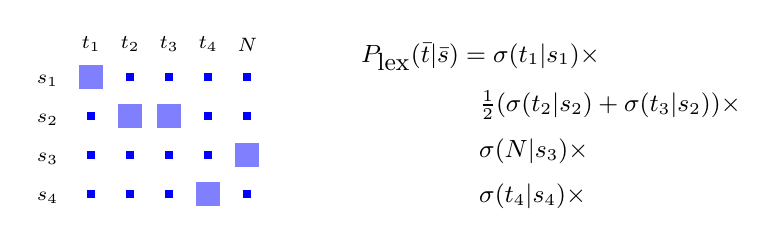
\begin{tikzpicture}

\tikzstyle{elementnode} = [rectangle,text=white,anchor=center]
\tikzstyle{srcnode} = [font=\small,anchor=south west]
\tikzstyle{tgtnode} = [left,font=\small,anchor=north east]
\tikzstyle{alignmentnode} = [rectangle,draw,minimum height=3.6*1.1cm,minimum width=0.36*1.1cm]
\tikzstyle{probnode} = [fill=blue!30,minimum width=0.4*1.1cm]
\tikzstyle{labelnode} = [above]

% alignment matrix1
\begin{scope}[scale=0.9,yshift=0.12in]
\foreach \i / \j / \c in
    {0/3/0.15, 1/3/0.15, 2/3/0.15, 3/3/0.15, 4/3/0.15,
    0/2/0.15, 1/2/0.15, 2/2/0.15, 3/2/0.15, 4/2/0.15,
    0/1/0.15, 1/1/0.15, 2/1/0.15, 3/1/0.15, 4/1/0.15,
    0/0/0.15, 1/0/0.15, 2/0/0.15, 3/0/0.15, 4/0/0.15}
    \node[elementnode,minimum size=0.6*1.1cm*\c,inner sep=0.1pt,fill=blue] (a\i\j) at (0.5*1.1cm*\i-5.4*0.5*1.1cm,0.5*1.1cm*\j-1.05*1.1cm) {};

% source
\node[srcnode] (tgt01) at (-5.9*0.5*1.1cm,-1.05*1.1cm+3.4*0.5*1.1cm) {\scriptsize{$t_1$}};
\node[srcnode] (tgt02) at ([xshift=0.5*1.1cm]tgt01.south west) {\scriptsize{$t_2$}};
\node[srcnode] (tgt03) at ([xshift=0.5*1.1cm]tgt02.south west) {\scriptsize{$t_3$}};
\node[srcnode] (tgt04) at ([xshift=0.5*1.1cm]tgt03.south west) {\scriptsize{$t_4$}};
\node[srcnode] (tgt05) at ([xshift=0.5*1.1cm]tgt04.south west) {\scriptsize{$N$}};

% target
\node[tgtnode] (src01) at (-6.0*0.5*1.1cm,-1.05*1.1cm+3.3*0.5*1.1cm) {\scriptsize{$s_1$}};
\node[tgtnode] (src02) at ([yshift=-0.5*1.1cm]src01.north east) {\scriptsize{$s_2$}};
\node[tgtnode] (src03) at ([yshift=-0.5*1.1cm]src02.north east) {\scriptsize{$s_3$}};
\node[tgtnode] (src04) at ([yshift=-0.5*1.1cm]src03.north east) {\scriptsize{$s_4$}};

% word alignment
\node[align=center,elementnode,minimum size=0.3cm,inner sep=0.1pt,fill=blue!50] (la1) at (a03) {};
\node[align=center,elementnode,minimum size=0.3cm,inner sep=0.1pt,fill=blue!50] (la2) at (a12) {};
\node[align=center,elementnode,minimum size=0.3cm,inner sep=0.1pt,fill=blue!50] (la3) at (a22) {};
\node[align=center,elementnode,minimum size=0.3cm,inner sep=0.1pt,fill=blue!50] (la4) at (a41) {};
\node[align=center,elementnode,minimum size=0.3cm,inner sep=0.1pt,fill=blue!50] (la5) at (a30) {};

\node[anchor=west] (f1) at ([xshift=4em,yshift=0.8em]a43.east) {\small{$\funp{P}_{\textrm{lex}}(\bar{t}|\bar{s})=\sigma (t_1|s_1)\times$}};
\node[anchor=north] (f2) at ([xshift=5.2em]f1.south) {\small{$\frac{1}{2}(\sigma (t_2|s_2)+\sigma (t_3|s_2))\times$}};
\node[anchor=north west] (f3) at (f2.south west) {\small{$\sigma (N|s_3)\times$}};
\node[anchor=north west] (f4) at (f3.south west) {\small{$\sigma (t_4|s_4)\times$}};

\end{scope}

\end{tikzpicture}
\end{center}
\caption{词汇翻译概率实例}
\label{fig:7-17}
\end{figure}
%-------------------------------------------

\parinterval 经过上面的介绍,可以从双语平行语料中把双语短语抽取出来,同时得到相应的翻译概率(即特征),组成{\small\bfnew{短语表}}\index{短语表}(Phrase Table)\index{Phrase Table}。图\ref{fig:7-18}展示了一个真实短语表的片段。其中包括源语言短语和目标语言短语,用|||进行分割。每个双语对应的得分,包括正向和反向的词汇翻译概率以及短语翻译概率,还包括词对齐信息(0-0、1-1)等其他信息。

%----------------------------------------------
\begin{figure}[htp]
\centering
%%%------------------------------------------------------------------------------------------------------------
%%% 展示短语表的内容
\begin{center}
\begin{tikzpicture}
\node [anchor=west] (s1) at (0,0) {\small{报告 认为 $\vert\vert\vert$ report holds that $\vert\vert\vert$ -2.62 -5.81 -0.91 -2.85 1 0 $\vert\vert\vert$ 4 $\vert\vert\vert$ 0-0 1-1 1-2}};
\node [anchor=west] (s2) at ([yshift=-1.2em]s1.west) {\small{,悲伤 $\vert\vert\vert$ , sadness $\vert\vert\vert$ -1.946 -3.659 0 -3.709 1 0 $\vert\vert\vert$ 1 $\vert\vert\vert$ 0-0 1-1}};
\node [anchor=west] (s3) at ([yshift=-1.2em]s2.west) {\small{,北京 等 $\vert\vert\vert$ , beijing , and other $\vert\vert\vert$ 0 -7.98 0 -3.84 1 0 $\vert\vert\vert$ 2 $\vert\vert\vert$ 0-0 1-1 2-2 2-3 2-4}};
\node [anchor=west] (s4) at ([yshift=-1.2em]s3.west) {\small{,北京 及 $\vert\vert\vert$ , beijing , and $\vert\vert\vert$ -0.69 -1.45 -0.92 -4.80 1 0  $\vert\vert\vert$ 2 $\vert\vert\vert$ 0-0 1-1 2-2}};
\node [anchor=west] (s5) at ([yshift=-1.2em]s4.west) {\small{一个 世界 $\vert\vert\vert$ one world $\vert\vert\vert$ 0 -1.725 0 -1.636 1 0 $\vert\vert\vert$ 2 $\vert\vert\vert$ 1-1 2-2}};
\node [anchor=west] (s7) at ([yshift=-1.1em]s5.west) {\small{...}};
\node [anchor=west] (s6) at ([yshift=1.0em]s1.west) {\small{...}};
\begin{pgfonlayer}{background}
\node [rectangle,inner sep=0.3em,fill=red!10] [fit = (s1) (s3) (s4) (s6) (s7)] (box1) {};
\end{pgfonlayer}
\end{tikzpicture}
\end{center}
\caption{短语表实例}
\label{fig:7-18}
\end{figure}
%-------------------------------------------

%----------------------------------------------------------------------------------------
%    NEW SECTION
%----------------------------------------------------------------------------------------
\sectionnewpage
\section{翻译调序建模}\label{subsection-7.4}

\parinterval 尽管已经知道了如何将一个源语言短语翻译成目标语言短语,但是想要获得一个高质量的译文,仅有互译的双语短语是远远不够的。

\parinterval 如图\ref{fig:7-19}所示,按照从左到右的顺序对一个句子“在/桌子/上/的/苹果”进行翻译,得到的译文“on the table the apple”的语序是不对的。虽然可以使用$n$-gram语言模型对语序进行建模,但是此处仍然需要用更加准确的方式描述目标语短语间的次序。一般,把这个问题称为短语调序,或者简称{\small\bfnew{调序}}\index{调序}(Reordering)\index{Reordering}。通常,基于短语的调序模型会作为判别式模型的特征参与到翻译过程中来。接下来,会介绍3 种不同的调序方法,分别是基于距离的调序、基于方向的调序(MSD模型)以及基于分类的调序。

%----------------------------------------------
\begin{figure}[htp]
\centering
%%%------------------------------------------------------------------------------------------------------------
%%% 调序模型1:基于距离的调序
\begin{center}
\begin{tikzpicture}

\begin{scope}[minimum height = 20pt]

\node[anchor=east] (s0) at (-0.5em, 0) {$\seq{s}$:};
\node[anchor=west,fill=green!20] (s1) at (0, 0) {\footnotesize{在 桌子 上 的}};
\node[anchor=west,fill=red!20] (s2) at ([xshift=1em]s1.east) {\footnotesize{苹果}};

\node[anchor=east] (t0) at (-0.5em, -1.5) {$\seq{t}$:};
\node[anchor=west,fill=red!20] (t1) at (0, -1.5) {\footnotesize{the apple}};
\node[anchor=west,fill=green!20] (t2) at ([xshift=1em]t1.east) {\footnotesize{on the table}};

\path[<->, thick] (s1.south) edge (t2.north);
\path[<->, thick] (s2.south) edge (t1.north);

\end{scope}
\end{tikzpicture}
\end{center}
\caption{基于短语翻译的调序}
\label{fig:7-19}
\end{figure}
%-------------------------------------------

%----------------------------------------------------------------------------------------
%    NEW SUB-SECTION
%----------------------------------------------------------------------------------------

\subsection{基于距离的调序}

\parinterval 基于距离的调序是最简单的一种调序模型。{\chaptersix}中所讨论的“扭曲度”本质上就是一种调序模型。只不过{\chaptersix}所涉及的扭曲度描述的是单词的调序问题,而这里需要把类似的概念推广到短语。

\parinterval 基于距离的调序的一个基本假设是:语言的翻译基本上都是顺序的,也就是,译文单词出现的顺序和源语言单词的顺序基本上是一致的。反过来说,如果译文和源语言单词(或短语)的顺序差别很大,就认为出现了调序。

\parinterval 基于距离的调序方法的核心思想就是度量当前翻译结果与顺序翻译之间的差距。对于译文中的第$i$个短语,令$\rm{start}_i$表示它所对应的源语言短语中第一个词所在的位置,$\rm{end}_i$表示它所对应的源语言短语中最后一个词所在的位置。于是,这个短语(相对于前一个短语)的调序距离为:
\begin{eqnarray}
dr & = & {\rm{start}}_i-{\rm{end}}_{i-1}-1
\label{eq:7-15}
\end{eqnarray}

\parinterval 在图\ref{fig:7-20}的例子中,“the apple”所对应的调序距离为4,“on the table”所对应的调序距离为$-5$。显然,如果两个源语短语按顺序翻译,则$\rm{start}_i = \rm{end}_{i-1} + 1$,这时调序距离为0。

%----------------------------------------------
\begin{figure}[htp]
\centering
%%%------------------------------------------------------------------------------------------------------------
%%% 调序模型1:基于距离的调序
\begin{center}
\begin{tikzpicture}

\begin{scope}[minimum height = 20pt]

\node[anchor=east] (s0) at (-0.5em, 0) {$\seq{s}$:};
\node[anchor=west,fill=green!20,draw,thick,rounded corners=0.3em] (s1) at (0, 0) {\small{在\ \ 桌子\ \ 上\ \ \;的}};
\node[anchor=south] (n1) at ([xshift=-2.5em,yshift=-0.5em]s1.north) {\small{1}};
\node[anchor=south] (n2) at ([xshift=-0.7em,yshift=-0.5em]s1.north) {\small{2}};
\node[anchor=south] (n3) at ([xshift=1.2em,yshift=-0.5em]s1.north) {\small{3}};
\node[anchor=south] (n4) at ([xshift=2.7em,yshift=-0.5em]s1.north) {\small{4}};
\node[anchor=west,fill=red!20,draw,thick,rounded corners=0.3em] (s2) at ([xshift=1em]s1.east) {\small{苹果}};
\node[anchor=south] (n5) at ([yshift=-0.5em]s2.north) {\small{5}};

\node[anchor=east] (t0) at (-0.5em, -1.5) {$\seq{t}$:};
\node[anchor=west,fill=red!20,draw,thick,rounded corners=0.3em] (t1) at (0, -1.5) {\small{the apple}};
\node[anchor=west,fill=green!20,draw,thick,rounded corners=0.3em] (t2) at ([xshift=1.3em]t1.east) {\small{on the table}};

\path[<->, thick] (s1.south) edge (t2.north);
\path[<->, thick] (s2.south) edge (t1.north);

\node[anchor=west] (target) at ([xshift=2em,yshift=2.3em]n5.east) {\small{目标短语位置}};
\node[anchor=west] (source) at ([xshift=0.3em]target.east) {\small{源短语位置}};
\node[anchor=west] (distance) at ([xshift=1.5em]source.east) {\small{距离}};

\node[anchor=north] (t1) at ([xshift=0em,yshift=-0.1em]target.south) {1};
\node[anchor=north] (t2) at ([yshift=-1.8em]t1.south) {2};

\node[anchor=north] (so1) at ([yshift=-0.1em]source.south) {5};
\node[anchor=north] (so2) at ([yshift=-1.8em]so1.south) {1-4};

\node[anchor=north] (d1) at ([xshift=-0.1em,yshift=-0.1em]distance.south) {+4};
\node[anchor=north] (d2) at ([yshift=-1.8em]d1.south) {-5};

\node[anchor=north west,fill=blue!20,draw,thick,rounded corners=0.3em] (m1) at ([xshift=-1em,yshift=-0.0em]t1.south west) {\small{$\rm{start}_1\ \ -\ \ \rm{end}_{0}\ \ -\ \ 1$\quad =\quad 5\ -\ 0\ -\ 1}};
\node[anchor=north west,fill=blue!20,draw,thick,rounded corners=0.3em] (m2) at ([xshift=-1em,yshift=-0.0em]t2.south west) {\small{$\rm{start}_2\ \ -\ \  \rm{end}_{1}\ \ -\ \ 1$\quad =\quad 1\ -\ 5\ -\ 1}};

\draw[-] ([xshift=0.08in]target.south west)--([xshift=2.4in]target.south west);

\draw[-,thick] (s1.north west)--([yshift=0.3in]s1.north west);
\draw[->,densely dotted,thick] ([yshift=0.3in]s1.north west)--([xshift=0.3in,yshift=0.3in]s1.north west);

\draw[-,thick] (s2.north west)--([yshift=0.3in]s2.north west);
\draw[->,densely dotted,thick] ([yshift=0.3in]s2.north west)--([xshift=-0.3in,yshift=0.3in]s2.north west);

\node[anchor=south] (ld1) at ([xshift=-0.5em,yshift=0.4em]n1.north) {\small{$dr= -5$}};
\node[anchor=south] (ld2) at ([xshift=6.5em,yshift=0.4em]n1.north) {\small{$dr= +4$}};


\end{scope}
\end{tikzpicture}
\end{center}
\caption{基于距离的调序}
\label{fig:7-20}
\end{figure}
%-------------------------------------------

\parinterval 如果把调序距离作为特征,一般会使用指数函数$f(dr) = a^{|dr|}$作为特征函数(或者调序代价的函数),其中$a$是一个参数,控制调序距离对整个特征值的影响。调序距离$dr$的绝对值越大,调序代价越高。基于距离的调序模型比较适用于像法语到英语翻译这样的任务,因为两种语言的语序基本上是一致的。但是,对于汉语到日语翻译,由于句子结构存在很大差异(日语是谓词后置,而汉语中谓词放在宾语前),使用基于距离的调序会带来一些问题。因此,具体应用时应该根据语言之间的差异性有选择地使用该模型。

%----------------------------------------------------------------------------------------
%    NEW SUB-SECTION
%----------------------------------------------------------------------------------------

\subsection{基于方向的调序}

\parinterval 基于方向的调序模型是另一种常用的调序模型。该模型是一种典型的词汇化调序模型,因此调序的结果会根据不同短语有所不同。简单来说,在两个短语目标语言端连续的情况下,该模型会判断两个双语短语在源语言端的调序情况,包含三种调序类型:顺序的单调翻译(M)、与前一个短语交换位置(S)、非连续翻译(D)。因此,这个模型也被称作MSD调序模型,也是Moses等经典的机器翻译系统所采用的调序模型\upcite{Koehn2007Moses}。

\parinterval 图\ref{fig:7-21}展示了这三种调序类型,当两个短语对在源语言和目标语言中都是按顺序排列时,它们就是单调的(如:从左边数前两个短语);如果对应的短语顺序在目标语中是反过来的,属于交换调序(如:从左边数第三和第四个短语);如果两个短语之间还有其他的短语,就是非连续调序(如:从右边数的前两个短语)。

%----------------------------------------------
\begin{figure}[htp]
\centering
%%%------------------------------------------------------------------------------------------------------------
%%% 调序模型2:MSD模型
\begin{center}
\begin{tikzpicture}

\tikzstyle{elementnode} = [rectangle,text=white,anchor=center]
\tikzstyle{srcnode} = [left,font=\small,anchor=south west]
\tikzstyle{tgtnode} = [left,font=\small,anchor=north east]
\tikzstyle{alignmentnode} = [rectangle,draw,minimum height=3.6*1.1cm,minimum width=0.36*1.1cm]
\tikzstyle{probnode} = [fill=blue!30,minimum width=0.4*1.1cm]
\tikzstyle{labelnode} = [above]

 alignment matrix
\begin{scope}[scale=0.92,yshift=0.12in]
\foreach \i / \j / \c in
    {0/5/0.15, 1/5/0.15, 2/5/0.15, 3/5/0.15, 4/5/0.15, 5/5/0.15, 6/5/0.15, 7/5/0.15,
    0/4/0.15, 1/4/0.15, 2/4/0.15, 3/4/0.15, 4/4/0.15, 5/4/0.15, 6/4/0.15, 7/4/0.15,
    0/3/0.15, 1/3/0.15, 2/3/0.15, 3/3/0.15, 4/3/0.15, 5/3/0.15, 6/3/0.15, 7/3/0.15,
    0/2/0.15, 1/2/0.15, 2/2/0.15, 3/2/0.15, 4/2/0.15, 5/2/0.15, 6/2/0.15, 7/2/0.15,
    0/1/0.15, 1/1/0.15, 2/1/0.15, 3/1/0.15, 4/1/0.15, 5/1/0.15, 6/1/0.15, 7/1/0.15,
    0/0/0.15, 1/0/0.15, 2/0/0.15, 3/0/0.15, 4/0/0.15, 5/0/0.15, 6/0/0.15, 7/0/0.15}
    \node[elementnode,minimum size=0.6*1.1cm*\c,inner sep=0.1pt,fill=blue] (a\i\j) at (0.5*1.1cm*\i-5.4*0.5*1.1cm,0.5*1.1cm*\j-0.05*1.1cm) {};

 source
\node[srcnode] (src1) at (-5.9*0.5*1.1cm,-1.05*1.1cm+7.5*0.5*1.1cm) {\scriptsize{$t_1$}};
\node[srcnode] (src2) at ([xshift=0.5*1.1cm]src1.south west) {\scriptsize{$t_2$}};
\node[srcnode] (src3) at ([xshift=0.5*1.1cm]src2.south west) {\scriptsize{$t_3$}};
\node[srcnode] (src4) at ([xshift=0.5*1.1cm]src3.south west) {\scriptsize{$t_4$}};
\node[srcnode] (src5) at ([xshift=0.5*1.1cm]src4.south west) {\scriptsize{$t_5$}};
\node[srcnode] (src6) at ([xshift=0.5*1.1cm]src5.south west) {\scriptsize{$t_6$}};
\node[srcnode] (src7) at ([xshift=0.5*1.1cm]src6.south west) {\scriptsize{$t_7$}};
\node[srcnode] (src8) at ([xshift=0.5*1.1cm]src7.south west) {\scriptsize{$t_8$}};

 target
\node[tgtnode] (tgt1) at (-6.0*0.5*1.1cm,-1.05*1.1cm+7.5*0.5*1.1cm) {\scriptsize{$s_1$}};
\node[tgtnode] (tgt2) at ([yshift=-0.5*1.1cm]tgt1.north east) {\scriptsize{$s_2$}};
\node[tgtnode] (tgt3) at ([yshift=-0.5*1.1cm]tgt2.north east) {\scriptsize{$s_3$}};
\node[tgtnode] (tgt4) at ([yshift=-0.5*1.1cm]tgt3.north east) {\scriptsize{$s_4$}};
\node[tgtnode] (tgt5) at ([yshift=-0.5*1.1cm]tgt4.north east) {\scriptsize{$s_5$}};
\node[tgtnode] (tgt6) at ([yshift=-0.5*1.1cm]tgt5.north east) {\scriptsize{$s_6$}};

 word alignment
\node[align=center,elementnode,minimum size=0.3cm,inner sep=0.1pt,fill=blue!50] (l05) at (a05) {};
\node[align=center,elementnode,minimum size=0.3cm,inner sep=0.1pt,fill=blue!50] (l14) at (a14) {};
\node[align=center,elementnode,minimum size=0.3cm,inner sep=0.1pt,fill=blue!50] (l24) at (a24) {};
\node[align=center,elementnode,minimum size=0.3cm,inner sep=0.1pt,fill=blue!50] (l31) at (a31) {};
\node[align=center,elementnode,minimum size=0.3cm,inner sep=0.1pt,fill=blue!50] (l32) at (a32) {};
\node[align=center,elementnode,minimum size=0.3cm,inner sep=0.1pt,fill=blue!50] (l43) at (a43) {};
\node[align=center,elementnode,minimum size=0.3cm,inner sep=0.1pt,fill=blue!50] (l53) at (a53) {};
\node[align=center,elementnode,minimum size=0.3cm,inner sep=0.1pt,fill=blue!50] (l63) at (a63) {};
\node[align=center,elementnode,minimum size=0.3cm,inner sep=0.1pt,fill=blue!50] (l70) at (a70) {};


{
\node [anchor=west] (p1line1) at ([xshift=3.5em,yshift=0.5em]a75.east) {\footnotesize{M(monotone):单调调序}};
\node [anchor=north west] (p1line2) at ([xshift=0,yshift=-1em]p1line1.south west) {\footnotesize{S(swap): 与前面一个短语}};
\node [anchor=north west] (p1line3) at ([xshift=3.8em]p1line2.south west) {\footnotesize{位置进行交换}};
\node [anchor=north west] (p1line4) at ([xshift=-3.5em,yshift=-1em]p1line3.south west) {\footnotesize{D(discontinuous):非连续调序}};

\node [anchor=east] (p1line5) at ([xshift=0em,yshift=3em]p1line4.east) {};
\node [anchor=east] (p1line6) at ([xshift=0em,yshift=7em]p1line4.east) {};

%\node [anchor=west] (p2line1) at ([xshift=4em]a73.east) {\footnotesize{$\bar{s}_j$: 真\ \ \ 好 \ \ }};
%\node [anchor=north west] (p2line2) at ([xshift=0]p2line1.south west) {\footnotesize{$\bar{t}_j$: very\ \ \ good\ \ \ \ \ \ \ \ }};

\begin{pgfonlayer}{background}
{
\node [rectangle,thick,inner sep=0.3em,fill=blue!40,drop shadow,fill opacity=0.85] [fit = (a05)] (phrase1) {};
\node [rectangle,thick,inner sep=0.3em,fill=blue!40,drop shadow,fill opacity=0.85] [fit = (a14) (a24)] (phrase2) {};
\node [rectangle,thick,inner sep=0.3em,fill=blue!40,drop shadow,fill opacity=0.85] [fit = (a31) (a32)] (phrase3) {};
\node [rectangle,thick,inner sep=0.3em,fill=blue!40,drop shadow,fill opacity=0.85] [fit = (a43) (a63)] (phrase4) {};
\node [rectangle,thick,inner sep=0.3em,fill=blue!40,drop shadow,fill opacity=0.85] [fit = (a70)] (phrase5) {};
\node [rectangle,inner sep=0.2em,fill=red!10] [fit = (p1line1) (p1line6)] (box1) {};
\node [rectangle,inner sep=0.2em,fill=ugreen!10] [fit = (p1line2) (p1line3) (p1line5)] (box2) {};
\node [rectangle,inner sep=0.2em,fill=orange!10] [fit = (p1line4)] (box3) {};
}
\end{pgfonlayer}

\node [circle,draw,anchor=south,inner sep=1pt,fill=red!20] (c1) at ([xshift=-0.5em]a05.north) {\scriptsize{m}};
\node [circle,draw,anchor=south,inner sep=1pt,fill=red!20] (c2) at ([xshift=-0.5em]a14.north) {\scriptsize{m}};
\node [circle,draw,anchor=north,inner sep=1pt,fill=orange!20] (c3) at ([xshift=0.1em]a24.south) {\scriptsize{d}};
\node [circle,draw,anchor=south,inner sep=2pt,fill=ugreen!20] (c4) at ([xshift=0.5em]a32.north) {\scriptsize{s}};
\node [circle,draw,anchor=north,inner sep=1pt,fill=orange!20] (c5) at ([xshift=0.5em]a63.south) {\scriptsize{d}};


\draw [->,thick] (a05.south east) -- (c1.315);
\draw [->,thick] ([xshift=-0.5em]a24.west) -- (c2.315);
\draw [->,thick] ([yshift=-0.7em]a32.south) .. controls +(west:1.3) and +(east:1.3) .. (c3.340);
\draw [->,thick] (a53.center) -- (c4.15);
\draw [->,thick] (a70.center) .. controls +(west:1.3) and +(east:1.3) .. (c5.340);
}
\end{scope}

\end{tikzpicture}
\end{center}
\caption{词汇化调序模型的三种调序类型}
\label{fig:7-21}
\end{figure}
%-------------------------------------------

\parinterval 对于每种调序类型,都可以定义一个调序概率,如下:
\begin{eqnarray}
\funp{P}(\seq{o}|\seq{s},\seq{t},\seq{a}) & = & \prod_{i=1}^{K} \funp{P}(o_i| \bar{s}_{a_i}, \bar{t}_i, a_{i-1}, a_i)
\label{eq:7-16}
\end{eqnarray}

\noindent 其中,$o_i$表示(目标语言)第$i$个短语的调序方向,$\seq{o}=\{o_i\}$表示短语序列的调序方向,$K$表示短语的数量。短语之间的调序概率是由双语短语以及短语对齐决定的,$o$表示调序的种类,可以取M、S、D 中的任意一种。而整个句子调序的好坏就是把相邻的短语之间的调序概率相乘(对应取log后的加法)。这样,公式\eqref{eq:7-16}把调序的好坏定义为新的特征,对于M、S、D总共就有三个特征。除了当前短语和前一个短语的调序特征,还可以定义当前短语和后一个短语的调序特征,即将上述公式中的$a_{i-1}$换成$a_{i+1}$。 于是,又可以得到三个特征。因此在MSD调序中总共可以有6个特征。

\parinterval 具体实现时,通常使用词对齐对两个短语间的调序关系进行判断。图\ref{fig:7-22}展示了这个过程。先判断短语的左上角和右上角是否存在词对齐,再根据其位置对调序类型进行划分。每个短语对应的调序概率都可以用相对频次估计进行计算。而MSD调序模型也相当于在短语表中的每个双语短语后添加6个特征。不过,调序模型一般并不会和短语表一起存储,因此在系统中通常会看到两个独立的模型文件,分别保存短语表和调序模型。

%----------------------------------------------
\begin{figure}[htp]
\centering
%------------------------------------------------------------------------------------------------------------
%%% 调序模型2:MSD模型
\begin{center}
\begin{tikzpicture}
\tikzstyle{elementnode} = [rectangle,anchor=center]
\tikzstyle{srcnode} = [font=\small,anchor=south west]
\tikzstyle{tgtnode} = [left,font=\small,anchor=north east]
\tikzstyle{alignmentnode} = [rectangle,draw,minimum height=3.6*1.1cm,minimum width=0.36*1.1cm]
\tikzstyle{probnode} = [fill=blue!30,minimum width=0.4*1.1cm]
\tikzstyle{labelnode} = [above]

% alignment matrix1
\begin{scope}[scale=0.9,yshift=0.12in]
\foreach \i / \j / \c in
    {0/5/0.15, 1/5/0.15, 2/5/0.15, 3/5/0.15, 4/5/0.15, 5/5/0.15,
    0/4/0.15, 1/4/0.15, 2/4/0.15, 3/4/0.15, 4/4/0.15, 5/4/0.15,
    0/3/0.15, 1/3/0.15, 2/3/0.15, 3/3/0.15, 4/3/0.15, 5/3/0.15,
    0/2/0.15, 1/2/0.15, 2/2/0.15, 3/2/0.15, 4/2/0.15, 5/2/0.15,
    0/1/0.15, 1/1/0.15, 2/1/0.15, 3/1/0.15, 4/1/0.15, 5/1/0.15,
    0/0/0.15, 1/0/0.15, 2/0/0.15, 3/0/0.15, 4/0/0.15, 5/0/0.15}
    \node[elementnode,minimum size=0.6*1.1cm*\c,inner sep=0.1pt,fill=blue] (a\i\j) at (0.5*1.1cm*\i-5.4*0.5*1.1cm,0.5*1.1cm*\j-1.05*1.1cm) {};

% source
\node[srcnode] (src01) at (-5.9*0.5*1.1cm,-1.05*1.1cm+5.4*0.5*1.1cm) {\scriptsize{$t_1$}};
\node[srcnode] (src02) at ([xshift=0.5*1.1cm]src01.south west) {\scriptsize{$t_2$}};
\node[srcnode] (src03) at ([xshift=0.5*1.1cm]src02.south west) {\scriptsize{$t_3$}};
\node[srcnode] (src04) at ([xshift=0.5*1.1cm]src03.south west) {\scriptsize{$t_4$}};
\node[srcnode] (src05) at ([xshift=0.5*1.1cm]src04.south west) {\scriptsize{$t_5$}};
\node[srcnode] (src06) at ([xshift=0.5*1.1cm]src05.south west) {\scriptsize{$t_6$}};

% target
\node[tgtnode] (tgt01) at (-6.0*0.5*1.1cm,-1.05*1.1cm+5.4*0.5*1.1cm) {\scriptsize{$s_1$}};
\node[tgtnode] (tgt02) at ([yshift=-0.5*1.1cm]tgt01.north east) {\scriptsize{$s_2$}};
\node[tgtnode] (tgt03) at ([yshift=-0.5*1.1cm]tgt02.north east) {\scriptsize{$s_3$}};
\node[tgtnode] (tgt04) at ([yshift=-0.5*1.1cm]tgt03.north east) {\scriptsize{$s_4$}};
\node[tgtnode] (tgt05) at ([yshift=-0.5*1.1cm]tgt04.north east) {\scriptsize{$s_5$}};
\node[tgtnode] (tgt06) at ([yshift=-0.5*1.1cm]tgt05.north east) {\scriptsize{$s_6$}};

%% alignment matrix2
\foreach \i / \j / \c in
    {0/5/0.15, 1/5/0.15, 2/5/0.15, 3/5/0.15, 4/5/0.15, 5/5/0.15,
    0/4/0.15, 1/4/0.15, 2/4/0.15, 3/4/0.15, 4/4/0.15, 5/4/0.15,
    0/3/0.15, 1/3/0.15, 2/3/0.15, 3/3/0.15, 4/3/0.15, 5/3/0.15,
    0/2/0.15, 1/2/0.15, 2/2/0.15, 3/2/0.15, 4/2/0.15, 5/2/0.15,
    0/1/0.15, 1/1/0.15, 2/1/0.15, 3/1/0.15, 4/1/0.15, 5/1/0.15,
    0/0/0.15, 1/0/0.15, 2/0/0.15, 3/0/0.15, 4/0/0.15, 5/0/0.15}
    \node[elementnode,minimum size=0.6*1.1cm*\c,inner sep=0.1pt,fill=blue] (b\i\j) at (0.5*1.1cm*\i+4*0.5*1.1cm,0.5*1.1cm*\j-1.05*1.1cm) {};

% source
\node[srcnode] (src11) at (3.5*0.5*1.1cm,-1.05*1.1cm+5.4*0.5*1.1cm) {\scriptsize{$t_1$}};
\node[srcnode] (src12) at ([xshift=0.5*1.1cm]src11.south west) {\scriptsize{$t_2$}};
\node[srcnode] (src13) at ([xshift=0.5*1.1cm]src12.south west) {\scriptsize{$t_3$}};
\node[srcnode] (src14) at ([xshift=0.5*1.1cm]src13.south west) {\scriptsize{$t_4$}};
\node[srcnode] (src15) at ([xshift=0.5*1.1cm]src14.south west) {\scriptsize{$t_5$}};
\node[srcnode] (src16) at ([xshift=0.5*1.1cm]src15.south west) {\scriptsize{$t_6$}};

% target
\node[tgtnode] (tgt11) at (3.4*0.5*1.1cm,-1.05*1.1cm+5.4*0.5*1.1cm) {\scriptsize{$s_1$}};
\node[tgtnode] (tgt12) at ([yshift=-0.5*1.1cm]tgt11.north east) {\scriptsize{$s_2$}};
\node[tgtnode] (tgt13) at ([yshift=-0.5*1.1cm]tgt12.north east) {\scriptsize{$s_3$}};
\node[tgtnode] (tgt14) at ([yshift=-0.5*1.1cm]tgt13.north east) {\scriptsize{$s_4$}};
\node[tgtnode] (tgt15) at ([yshift=-0.5*1.1cm]tgt14.north east) {\scriptsize{$s_5$}};
\node[tgtnode] (tgt16) at ([yshift=-0.5*1.1cm]tgt15.north east) {\scriptsize{$s_6$}};


% word alignment
\node[align=center,elementnode,minimum size=0.3cm,inner sep=0.1pt,fill=blue!50] (la1) at (a23) {};
\node[align=center,elementnode,minimum size=0.3cm,inner sep=0.1pt,fill=blue!50] (la2) at (a22) {};
\node[align=center,elementnode,minimum size=0.3cm,inner sep=0.1pt,fill=blue!50] (la3) at (a31) {};
{
\node[align=center,elementnode,minimum size=0.5cm,inner sep=0.1pt,fill=red!50] (la4) at (a14) {M};
}

{
\node[align=center,elementnode,minimum size=0.5cm,inner sep=0.1pt,fill=ugreen!50] (la5) at (a44) {S};
}

\node[align=center,elementnode,minimum size=0.3cm,inner sep=0.1pt,fill=blue!50] (lb1) at (b23) {};
\node[align=center,elementnode,minimum size=0.3cm,inner sep=0.1pt,fill=blue!50] (lb2) at (b22) {};
\node[align=center,elementnode,minimum size=0.3cm,inner sep=0.1pt,fill=blue!50] (lb3) at (b31) {};
{
\node[align=center,elementnode,minimum size=0.3cm,inner sep=0.1pt,fill=red!50] (lb4) at (b05) {};
\node[align=center,elementnode,minimum size=0.3cm,inner sep=0.1pt,fill=red!50] (lb5) at (b14) {};
}
{
\node[align=center,elementnode,minimum size=0.3cm,inner sep=0.1pt,fill=ugreen!50] (lb6) at (b45) {};
\node[align=center,elementnode,minimum size=0.3cm,inner sep=0.1pt,fill=ugreen!50] (lb7) at (b54) {};
}

\begin{pgfonlayer}{background}
\node [rectangle,thick,inner sep=0.4em,fill=blue!40,drop shadow,fill opacity=0.85] [fit = (a23) (a31)] (phrase1) {};
\node [rectangle,thick,inner sep=0.4em,fill=blue!40,drop shadow,fill opacity=0.85] [fit = (b23) (b31)] (phrase2) {};
{
\node [rectangle,thick,inner sep=0.4em,fill=red!40,drop shadow,fill opacity=0.85] [fit = (b05) (b14)] (phrase3) {};
}
{
\node [rectangle,thick,inner sep=0.4em,fill=ugreen!40,drop shadow,fill opacity=0.85] [fit = (b45) (b54)] (phrase4) {};
}
\end{pgfonlayer}

{
\node[anchor=north] (s1) at ([xshift=0.6em,yshift=0.1em]b45.east) {S};
}
{
\node[anchor=north] (m1) at ([xshift=0.6em,yshift=0.1em]b05.east) {M};
}

\node[anchor=north] (l1) at ([xshift=1.8em,yshift=-0.5em]a10.south) {\small{基于词}};
\node[anchor=north] (l2) at ([xshift=2.2em,yshift=-0.5em]b10.south) {\small{基于短语}};

\end{scope}

\end{tikzpicture}
\end{center}
\caption{调序类型的判断}
\label{fig:7-22}
\end{figure}
%-------------------------------------------

%----------------------------------------------------------------------------------------
%    NEW SUB-SECTION
%----------------------------------------------------------------------------------------

\subsection{基于分类的调序}

\parinterval 在MSD调序中,双语短语所对应的调序概率$\funp{P}(o_i| \bar{s}_{a_i}, \bar{t}_i, a_{i-1}, a_i)$是用极大似然估计方法进行计算的。但是,这种方法也会面临数据稀疏问题,同时对调序产生影响的细致特征也没有考虑进来。另一种有效的方法是直接用统计分类模型对调序进行建模,比如,可以使用最大熵、SVM等分类器输出调序概率或者得分\upcite{xiong2006maximum,och2004alignment,DBLP:conf/naacl/KumarB05}。对于基于分类的调序模型,有两方面问题需要考虑:

\begin{itemize}
\vspace{0.5em}
\item 训练样本的生成。可以把M、S、D看作是类别标签,把所对应的短语及短语对齐信息看作是输入。这样就得到了大量分类器训练所需的样本。
\vspace{0.5em}
\item 分类特征设计。这部分是传统统计机器学习中的重要组成部分,好的特征会对分类结果产生很大影响。在调序模型中,一般直接使用单词作为特征,比如用短语的第一个单词和最后一个单词作为特征就可以达到很好的效果。
\vspace{0.5em}
\end{itemize}

\parinterval 随着神经网络方法的兴起,也可以考虑使用多层神经网络构建调序模型\upcite{li-etal-2014-neural}。这时,可以把短语直接送入一个神经网络,之后由神经网络完成对特征的抽取和表示,并输出最终的调序模型得分。

%----------------------------------------------------------------------------------------
%    NEW SECTION
%----------------------------------------------------------------------------------------
\sectionnewpage
\section{翻译特征}

\parinterval 基于短语的模型使用判别式模型对翻译推导进行建模,给定双语句对$(\seq{s},\seq{t})$,每个翻译推导$d$都有一个模型得分,由$M$个特征线性加权得到,记为$\textrm{score}(d,\seq{t},\seq{s}) = \sum_{i=1}^{M} \lambda_i \cdot h_i (d,\seq{t},\seq{s})$,其中$\lambda_i$表示特征权重,$h_i (d,\seq{t},\seq{s})$表示特征函数(简记为$h_i (d)$)。这些特征包含刚刚介绍过的短语翻译概率、调序模型得分等,除此之外,还包含语言模型等其他特征,它们共同组成了特征集合。这里列出了基于短语的模型中的一些基础特征:

\begin{itemize}
\vspace{0.5em}
\item 短语翻译概率(取对数),包含正向翻译概率$\textrm{log}(\funp{P}(\bar{t}|\bar{s}))$和反向翻译概率$\textrm{log}(\funp{P}(\bar{s}$\\$|\bar{t}))$,它们是基于短语的模型中最主要的特征。
\vspace{0.5em}
\item 词汇化翻译概率(取对数),同样包含正向词汇化翻译概率$\textrm{log}(\funp{P}_{\textrm{lex}}(\bar{t}|\bar{s}))$和反向词汇化翻译概率$\textrm{log}(\funp{P}_{\textrm{lex}}(\bar{s}|\bar{t}))$,它们用来描述双语短语中单词间对应的好坏。
\vspace{0.5em}
\item $n$-gram语言模型,用来度量译文的流畅程度,可以通过大规模目标端单语数据得到。
\vspace{0.5em}
\item 译文长度,避免模型倾向于短译文,同时让系统自动学习对译文长度的偏好。
\vspace{0.5em}
\item 翻译规则数量,为了避免模型仅使用少量特征构成翻译推导(规则数量少,短语翻译概率相乘的因子也会少,得分一般会大一些),同时让系统自动学习对规则数量的偏好。
\vspace{0.5em}
\item 被翻译为空的源语言单词数量。注意,空翻译特征有时也被称作{\small\bfnew{有害特征}}\index{有害特征}(Evil Feature\index{Evil Feature}),这类特征在一些数据上对BLEU有很好的提升作用,但会造成人工评价结果的下降,需要谨慎使用。
\vspace{0.5em}
\item 基于MSD的调序模型,包括与前一个短语的调序模型$f_{\textrm{M-pre}}(d)$\ 、$f_{\textrm{S-pre}}(d)$\ 、$f_{\textrm{D-pre}}(d)$和与后一个短语的调序模型$f_{\textrm{M-fol}}(d)$\ 、$f_{\textrm{S-fol}}(d)$\ 、$f_{\textrm{D-fol}}(d)$,共6个特征。
\vspace{0.5em}
\end{itemize}

%----------------------------------------------------------------------------------------
%    NEW SECTION
%----------------------------------------------------------------------------------------

\sectionnewpage
\section{最小错误率训练}\label{section-7.6}

\parinterval 除了特征设计,统计机器翻译也需要找到每个特征所对应的最优权重$\lambda_i$。这也就是机器学习中所说的模型训练问题。不过,需要指出的是,统计机器翻译关于模型训练的定义与传统机器学习稍有不同。在统计机器翻译中,短语抽取和翻译概率的估计被看作是{\small\bfnew{模型训练}}\index{模型训练}(Model Training)\index{Model Training},也就是说这里的模型训练是指特征函数的学习;而特征权重的训练,一般被称作{\small\bfnew{权重调优}}\index{权重调优}(Weight Tuning)\index{Weight Tuning},而这个过程才真正对应了传统机器学习(如分类任务)中的模型训练过程。在本章中,如果没有特殊说明,权重调优就是指特征权重的学习,模型训练是指短语抽取和特征函数的学习。

\parinterval 想要得到最优的特征权重,最简单的方法是枚举所有特征权重可能的取值,然后评价每组权重所对应的翻译性能,最后选择最优的特征权重作为调优的结果。但是特征权重是一个实数值,因此可以考虑把实数权重进行量化,即把权重看作是在固定间隔上的取值,比如,每隔0.01取值。即使是这样,同时枚举多个特征的权重也是非常耗时的工作,当特征数量增多时这种方法的效率仍然很低。

\parinterval 这里介绍一种更加高效的特征权重调优方法$\ \dash \ ${\small\bfnew{最小错误率训练}}\index{最小错误率训练}(Minimum Error Rate Training\index{Minimum Error Rate Training},MERT)。最小错误率训练是统计机器翻译发展中代表性工作,也是机器翻译领域原创的重要技术方法之一\upcite{DBLP:conf/acl/Och03}。最小错误率训练假设:翻译结果相对于标准答案的错误是可度量的,进而可以通过降低错误数量的方式来找到最优的特征权重。假设有样本集合$S = \{(s^{[1]},\seq{r}^{[1]}),...,(s^{[N]},\seq{r}^{[N]})\}$,$s^{[i]}$为样本中第$i$个源语言句子,$\seq{r}^{[i]}$为相应的参考译文。注意,$\seq{r}^{[i]}$ 可以包含多个参考译文。$S$通常被称为{\small\bfnew{调优集合}}\index{调优集合}(Tuning Set)\index{Tuning Set}。对于$S$中的每个源语句子$s^{[i]}$,机器翻译模型会解码出$n$-best推导$\hat{\seq{d}}^{[i]} = \{\hat{d}_{j}^{[i]}\}$,其中$\hat{d}_{j}^{[i]}$表示对于源语言句子$s^{[i]}$得到的第$j$个最好的推导。$\{\hat{d}_{j}^{[i]}\}$可以被定义如下:

\begin{eqnarray}
\{\hat{d}_{j}^{[i]}\} & = & \arg\max_{\{d_{j}^{[i]}\}} \sum_{i=1}^{M} \lambda_i \cdot h_i (d,\seq{t}^{[i]},\seq{s}^{[i]})
\label{eq:7-17}
\end{eqnarray}

\parinterval 对于每个样本都可以得到$n$-best推导集合,整个数据集上的推导集合被记为$\hat{\seq{D}} = \{\hat{\seq{d}}^{[1]},...,\hat{\seq{d}}^{[N]}\}$。进一步,令所有样本的参考译文集合为$\seq{R} = \{\seq{r}^{[1]},...,\seq{r}^{[N]}\}$。最小错误率训练的目标就是降低$\hat{\seq{D}}$相对于$\seq{R}$的错误。也就是,通过调整不同特征的权重$\lambda = \{ \lambda_i \}$,让错误率最小,形式化描述为:
\begin{eqnarray}
\hat{\lambda} & = & \arg\min_{\lambda} \textrm{Error}(\hat{\seq{D}},\seq{R})
\label{eq:7-18}
\end{eqnarray}
%公式--------------------------------------------------------------------

\noindent 其中,\textrm{Error}$(\cdot)$是错误率函数。\textrm{Error}$(\cdot)$的定义方式有很多,一般来说\textrm{Error}$(\cdot)$会与机器翻译的评价指标相关,例如,词错误率(WER)、位置错误率(PER)、BLEU 值、NIST值等都可以用于\textrm{Error}$(\cdot)$的定义。这里使用$1-$BLEU作为错误率函数,即$\textrm{Error}(\hat{\seq{D}},\seq{R}) = 1 - \textrm{BLEU}(\hat{\seq{D}},\seq{R})$。则公式\eqref{eq:7-18}可改写为:
%公式--------------------------------------------------------------------
\begin{eqnarray}
\hat{\lambda} &=& \arg\min_{\lambda}\ (1 - \textrm{BLEU}(\hat{\seq{D}},\seq{R}))   \nonumber \\
&=& \arg\max_{\lambda} \textrm{BLEU}(\hat{\seq{D}},\seq{R})
\label{eq:7-19}
\end{eqnarray}
%公式--------------------------------------------------------------------

\parinterval 需要注意的是, BLEU本身是一个不可微分函数。因此,无法使用梯度下降等方法对式\eqref{eq:7-19}进行求解。那么如何能快速得到最优解?这里会使用一种特殊的优化方法,称作{\small\bfnew{线搜索}}\index{线搜索}(Line Search)\index{Line Search},它是Powell搜索的一种形式\upcite{powell1964an}。这种方法也构成了最小错误率训练的核心。

\parinterval 首先,重新看一下特征权重的搜索空间。按照前面的介绍,如果要进行暴力搜索,需要把特征权重的取值按小的间隔进行划分。这样,所有特征权重的取值可以用图\ref{fig:7-23}的网格来表示。

%----------------------------------------------
\begin{figure}[htp]
\centering
\begin{tikzpicture}
\begin{scope}[scale=0.55] 
{\tiny
\draw[step=1,help lines,color=black] grid (4,4); 

\draw [-](n1) (0,4) -- (0,4.4);
\draw [-](n2) (1,4) -- (1,4.4);
\draw [-](n3) (2,4) -- (2,4.4);
\draw [-](n4) (3,4) -- (3,4.4);
\draw [-](n5) (4,4) -- (4,4.4);

\node[anchor=north] (y2) at (-5.3em,1.5) {0.01};
\node[anchor=north] (y1) at ([xshift=0em,yshift=-3.3em]y2.south) {0.00};
\node[anchor=north] (y3) at ([xshift=0em,yshift=4.5em]y2.north) {0.02};
\node[anchor=north] (y4) at ([xshift=0em,yshift=6.6em]y3.north) {$\vdots$};
\node[anchor=north] (y5) at ([xshift=0em,yshift=2em]y4.north) {1.00};

\node[anchor=north] (x1) at (1em,-3em) {$\lambda_1$};
\node[anchor=north] (x2) at ([xshift=4.5em,yshift=0em]x1.north) {$\lambda_2$};
\node[anchor=north] (x3) at ([xshift=4em,yshift=-1em]x2.north) {$...$};
\node[anchor=north] (x4) at ([xshift=5em,yshift=1em]x3.north) {$\lambda_{M-1}$};
\node[anchor=north] (x5) at ([xshift=5em,yshift=0em]x4.north) {$\lambda_M$};

\draw[decorate,decoration={brace}](0,4.7) --(4,4.7) node [xshift=-4em,yshift=1.5em,align=center](label1) {M个特征函数};	

\draw[decorate,decoration={brace}](4.5,4.3) --(4.5,0) node [xshift=2.3em,yshift=6.8em,align=center](label2) {V种};	
\node[anchor=north] (label3) at ([xshift=0em,yshift=-2.5em]label2.north) {取值};	
}

\node[anchor=north] (l1) at ([xshift=0em,yshift=-1.0em]x3.south) {\small{(a)搜索空间}};
\end{scope}

\begin{scope}[scale=0.55,xshift=3.2in] 
{\tiny
\draw[step=1,help lines,color=black] grid (4,4); 

\node[anchor=north] (y2) at (-5.3em,1.5) {0.01};
\node[anchor=north] (y1) at ([xshift=0em,yshift=-3.3em]y2.south) {0.00};
\node[anchor=north] (y3) at ([xshift=0em,yshift=4.5em]y2.north) {0.02};
\node[anchor=north] (y4) at ([xshift=0em,yshift=6.6em]y3.north) {$\vdots$};
\node[anchor=north] (y5) at ([xshift=0em,yshift=2em]y4.north) {1.00};

\node[anchor=north] (x1) at (1em,-3em) {$\lambda_1$};
\node[anchor=north] (x2) at ([xshift=4.5em,yshift=0em]x1.north) {$\lambda_2$};
\node[anchor=north] (x3) at ([xshift=4em,yshift=-1em]x2.north) {$...$};
\node[anchor=north] (x4) at ([xshift=5em,yshift=1em]x3.north) {$\lambda_{M-1}$};
\node[anchor=north] (x5) at ([xshift=5em,yshift=0em]x4.north) {$\lambda_M$};

\draw [-](n1) (0,4) -- (0,4.4);
\draw [-](n2) (1,4) -- (1,4.4);
\draw [-](n3) (2,4) -- (2,4.4);
\draw [-](n4) (3,4) -- (3,4.4);
\draw [-](n5) (4,4) -- (4,4.4);

\node [anchor=center,draw,circle,inner sep=1.5pt,blue!30,fill=blue!30] (r11) at (0,1) {};
\node [anchor=center,draw,circle,inner sep=1.5pt,blue!30,fill=blue!30] (r12) at (1,2) {};
\node [anchor=center,draw,circle,inner sep=1.5pt,blue!30,fill=blue!30] (r13) at (2,1) {};
\node [anchor=center,draw,circle,inner sep=1.5pt,blue!30,fill=blue!30] (r14) at (3,2) {};
\node [anchor=center,draw,circle,inner sep=1.5pt,blue!30,fill=blue!30] (r15) at (4,4) {};

\draw [-,very thick,blue!50] (0,1) -- (1,2) -- (2,1) -- (3,2) -- (4,4);

\node[anchor=north] (p1) at (5.7,4.3) {\scriptsize{$\leftarrow$ \textbf{path}:}};

\node[anchor=north] (e1) at ([xshift=0,yshift=-0.4em]p1.south) {$w_1 = 0.01$};
\node[anchor=north] (e2) at ([xshift=0,yshift=-0.8em]e1.south) {$w_2 = 0.02$};
\node[anchor=north] (e3) at ([xshift=0,yshift=0.4em]e2.south) {$\vdots$};
\node[anchor=north] (e4) at ([xshift=0,yshift=-0.2em]e3.south) {$w_M = 1.00$};
}

\node[anchor=north] (l1) at ([xshift=0em,yshift=-1.0em]x3.south) {\small{(b)一条搜索路径}};
\end{scope}

\begin{scope}[scale=0.55,xshift=6.8in] 
{\tiny
\draw[step=1,help lines,color=black] grid (4,4); 

\node[anchor=north] (y2) at (-5.3em,1.5) {0.01};
\node[anchor=north] (y1) at ([xshift=0em,yshift=-3.3em]y2.south) {0.00};
\node[anchor=north] (y3) at ([xshift=0em,yshift=4.5em]y2.north) {0.02};
\node[anchor=north] (y4) at ([xshift=0em,yshift=6.6em]y3.north) {$\vdots$};
\node[anchor=north] (y5) at ([xshift=0em,yshift=2em]y4.north) {1.00};

\node[anchor=north] (x1) at (1em,-3em) {$\lambda_1$};
\node[anchor=north] (x2) at ([xshift=4.5em,yshift=0em]x1.north) {$\lambda_2$};
\node[anchor=north] (x3) at ([xshift=4em,yshift=-1em]x2.north) {$...$};
\node[anchor=north] (x4) at ([xshift=5em,yshift=1em]x3.north) {$\lambda_{M-1}$};
\node[anchor=north] (x5) at ([xshift=5em,yshift=0em]x4.north) {$\lambda_M$};

\draw [-](n1) (0,4) -- (0,4.4);
\draw [-](n2) (1,4) -- (1,4.4);
\draw [-](n3) (2,4) -- (2,4.4);
\draw [-](n4) (3,4) -- (3,4.4);
\draw [-](n5) (4,4) -- (4,4.4);

\node [anchor=center,draw,circle,inner sep=1.5pt,blue!30,fill=blue!30] (r11) at (0,1) {};
\node [anchor=center,draw,circle,inner sep=1.5pt,blue!30,fill=blue!30] (r12) at (1,2) {};
\node [anchor=center,draw,circle,inner sep=1.5pt,blue!30,fill=blue!30] (r13) at (2,1) {};
\node [anchor=center,draw,circle,inner sep=1.5pt,blue!30,fill=blue!30] (r14) at (3,2) {};
\node [anchor=center,draw,circle,inner sep=1.5pt,blue!30,fill=blue!30] (r15) at (4,4) {};

\node [anchor=center,draw,circle,inner sep=1.5pt,ugreen!30,fill=ugreen!30] (r21) at (0,2) {};
\node [anchor=center,draw,circle,inner sep=1.5pt,ugreen!30,fill=ugreen!30] (r22) at (1,3) {};
\node [anchor=center,draw,circle,inner sep=1.5pt,ugreen!30,fill=ugreen!30] (r23) at (2,4) {};
\node [anchor=center,draw,circle,inner sep=1.5pt,ugreen!30,fill=ugreen!30] (r24) at (3,0) {};
\node [anchor=center,draw,circle,inner sep=1.5pt,ugreen!30,fill=ugreen!30] (r25) at (4,2) {};

\node [anchor=center,draw,circle,inner sep=1.5pt,red!30,fill=red!30] (r31) at (0,4) {};
\node [anchor=center,draw,circle,inner sep=1.5pt,red!30,fill=red!30] (r32) at (1,3) {};
\node [anchor=center,draw,circle,inner sep=1.5pt,red!30,fill=red!30] (r33) at (2,2) {};
\node [anchor=center,draw,circle,inner sep=1.5pt,red!30,fill=red!30] (r34) at (3,3) {};
\node [anchor=center,draw,circle,inner sep=1.5pt,red!30,fill=red!30] (r35) at (4,1) {};

\draw [-,very thick,blue!50] (0,1) -- (1,2) -- (2,1) -- (3,2) -- (4,4);
\draw [-,very thick,ugreen!50] (0,2) -- (1,3) -- (2,4) -- (3,0) -- (4,2);
\draw [-,very thick,red!50] (0,4) -- (1,3) -- (2,2) -- (3,3) -- (4,1);

\draw[decorate,decoration={brace}](4.5,4.3) --(4.5,0) node [xshift=2.3em,yshift=6.5em,align=center](label1) {$M^V$};	
\node[anchor=north] (label2) at ([xshift=0em,yshift=-2.5em]label1.north) {种组合};
}

\node[anchor=north] (l1) at ([xshift=0em,yshift=-1.0em]x3.south) {\small{(c)多条搜索路径}};
\end{scope}
\end{tikzpicture}
\caption{特征权重的搜索空间表示}
\label{fig:7-23}
\end{figure}
%-------------------------------------------

\parinterval 其中横坐标为所有的$M$个特征函数,纵坐标为权重可能的取值。假设每个特征都有$V$种取值,那么遍历所有特征权重取值的组合有$M^V$种。每组$\lambda = \{\lambda_i\}$的取值实际上就是一个贯穿所有特征权重的折线,如图\ref{fig:7-23}中间蓝线所展示的路径。当然,可以通过枚举得到很多这样的折线(图\ref{fig:7-23}右)。假设计算BLEU的时间开销为$B$,那么遍历所有的路径的时间复杂度为$O(M^V \cdot B)$,由于$V$可能很大,而且$B$往往也无法忽略,因此这种计算方式的时间成本是极高的。如果考虑对每一组特征权重都需要重新解码得到$n$-best译文,那么基于这种简单枚举的方法是无法使用的。

\parinterval 对全搜索的一种改进是使用局部搜索。循环处理每个特征,每一次只调整一个特征权重的值,找到使BLEU达到最大的权重。反复执行该过程,直到模型达到稳定状态(例如BLEU不再降低)。

\parinterval 图\ref{fig:7-24}左侧展示了这种方法。其中蓝色部分为固定的权重,相应的虚线部分为当前权重所有可能的取值,这样搜索一个特征权重的时间复杂度为$O(V \cdot B)$。而整个算法的时间复杂度为$O(L \cdot V \cdot B)$,其中$L$为循环访问特征的总次数。这种方法也被称作{\small\bfnew{格搜索}}\index{格搜索}(Grid Search)\index{Grid Search}。

%----------------------------------------------
\begin{figure}[htp]
\centering
\begin{tikzpicture}
\begin{scope}[scale=0.62] 
{\tiny
\draw[step=1,help lines,color=black] (0,0) grid (4,4); 

\node[anchor=north] (y2) at (-5.3em,1.5) {0.01};
\node[anchor=north] (y1) at ([xshift=0em,yshift=-3.3em]y2.south) {0.00};
\node[anchor=north] (y3) at ([xshift=0em,yshift=4.5em]y2.north) {0.02};
\node[anchor=north] (y4) at ([xshift=0em,yshift=6.6em]y3.north) {$\vdots$};
\node[anchor=north] (y5) at ([xshift=0em,yshift=2em]y4.north) {1.00};

\node[anchor=north] (x1) at (1em,-3em) {$\lambda_1$};
\node[anchor=north] (x2) at ([xshift=4.5em,yshift=0em]x1.north) {$\lambda_2$};
\node[anchor=north] (x3) at ([xshift=4em,yshift=-1em]x2.north) {$...$};
\node[anchor=north] (x4) at ([xshift=5em,yshift=1em]x3.north) {$\lambda_{M-1}$};
\node[anchor=north] (x5) at ([xshift=5em,yshift=0em]x4.north) {$\lambda_M$};

\draw [-](n1) (0,4) -- (0,4.4);
\draw [-](n2) (1,4) -- (1,4.4);
\draw [-](n3) (2,4) -- (2,4.4);
\draw [-](n4) (3,4) -- (3,4.4);
\draw [-](n5) (4,4) -- (4,4.4);

\node [anchor=center,draw,circle,inner sep=1.5pt,red!30,fill=red!30] (r31) at (2,4) {};
\node [anchor=center,draw,circle,inner sep=1.5pt,red!30,fill=red!30] (r32) at (2,0) {};
\node [anchor=center,draw,circle,inner sep=1.5pt,red!30,fill=red!30] (r33) at (2,2) {};
\node [anchor=center,draw,circle,inner sep=1.5pt,red!30,fill=red!30] (r34) at (2,3) {};
\node [anchor=center,draw,circle,inner sep=1.5pt,red!30,fill=red!30] (r35) at (2,1) {};

\node [anchor=center,draw,circle,inner sep=1.5pt,blue!30,fill=blue!30] (f11) at ([xshift=0em,yshift=23em]y2.north) {};
\node[anchor=south] (f12) at ([xshift=8.5em,yshift=-1em]f11.south) {\scriptsize{固定的权重}};
\node [anchor=center,draw,circle,inner sep=1.5pt,ugreen!50,fill=ugreen!50] (f21) at ([xshift=0em,yshift=-4em]f11.north) {};
\node[anchor=south] (f22) at ([xshift=8.5em,yshift=-1em]f21.south) {\scriptsize{有效取值点}};
\node [anchor=center,draw,circle,inner sep=1.5pt,red!30,fill=red!30] (f31) at ([xshift=0em,yshift=-4em]f21.north) {};
\node[anchor=south] (f32) at ([xshift=8.5em,yshift=-1em]f31.south) {\scriptsize{无效取值点}};

\draw [-,very thick,red!50, dashed] (1,2) -- (2,4) -- (3,2) -- (2,3) -- (1,2) -- (3,2) -- (2,1) -- (1,2) -- (2,0) -- (3,2);
\draw [-,very thick,blue!50] (0,1) -- (1,2);
\draw [-,very thick,blue!50] (3,2) -- (4,4);

\node [anchor=center,draw,circle,inner sep=1.5pt,blue!30,fill=blue!30] (r11) at (0,1) {};
\node [anchor=center,draw,circle,inner sep=1.5pt,blue!30,fill=blue!30] (r12) at (1,2) {};
\node [anchor=center,draw,circle,inner sep=1.5pt,blue!30,fill=blue!30] (r14) at (3,2) {};
\node [anchor=center,draw,circle,inner sep=1.5pt,blue!30,fill=blue!30] (r15) at (4,4) {};
}
\end{scope}

\begin{scope}[scale=0.62,xshift=3in] 
{\tiny
\draw[step=1,help lines,color=black] (0,0) grid (4,4); 

\node[anchor=north] (y2) at (-5.3em,1.5) {0.01};
\node[anchor=north] (y1) at ([xshift=0em,yshift=-3.3em]y2.south) {0.00};
\node[anchor=north] (y3) at ([xshift=0em,yshift=4.5em]y2.north) {0.02};
\node[anchor=north] (y4) at ([xshift=0em,yshift=6.6em]y3.north) {$\vdots$};
\node[anchor=north] (y5) at ([xshift=0em,yshift=2em]y4.north) {1.00};

\node[anchor=north] (x1) at (1em,-3em) {$\lambda_1$};
\node[anchor=north] (x2) at ([xshift=4.5em,yshift=0em]x1.north) {$\lambda_2$};
\node[anchor=north] (x3) at ([xshift=4em,yshift=-1em]x2.north) {$...$};
\node[anchor=north] (x4) at ([xshift=5em,yshift=1em]x3.north) {$\lambda_{M-1}$};
\node[anchor=north] (x5) at ([xshift=5em,yshift=0em]x4.north) {$\lambda_M$};

\draw [-](n1) (0,4) -- (0,4.4);
\draw [-](n2) (1,4) -- (1,4.4);
\draw [-](n3) (2,4) -- (2,4.4);
\draw [-](n4) (3,4) -- (3,4.4);
\draw [-](n5) (4,4) -- (4,4.4);

\node [anchor=center,draw,circle,inner sep=1.5pt,red!30,fill=red!30] (r31) at (2,4) {};
\node [anchor=center,draw,circle,inner sep=1.5pt,red!30,fill=red!30] (r32) at (2,0) {};
\node [anchor=center,draw,circle,inner sep=1.5pt,red!30,fill=red!30] (r33) at (2,2) {};
\node [anchor=center,draw,circle,inner sep=1.5pt,red!30,fill=red!30] (r35) at (2,1) {};

\node [anchor=center,draw,circle,inner sep=1.5pt,ugreen!50,fill=ugreen!50] (r34) at (2,3) {};

\draw [-,very thick,red!50, dashed] (1,2) -- (2,4) -- (3,2) -- (2,3) -- (1,2) -- (3,2) -- (2,1) -- (1,2) -- (2,0) -- (3,2);
\draw [-,very thick,blue!50] (0,1) -- (1,2);
\draw [-,very thick,blue!50] (3,2) -- (4,4);
\draw [-,very thick,ugreen!50, dashed] (1,2) -- (2,3) -- (3,2);

\node [anchor=center,draw,circle,inner sep=1.5pt,blue!30,fill=blue!30] (r11) at (0,1) {};
\node [anchor=center,draw,circle,inner sep=1.5pt,blue!30,fill=blue!30] (r12) at (1,2) {};
\node [anchor=center,draw,circle,inner sep=1.5pt,blue!30,fill=blue!30] (r14) at (3,2) {};
\node [anchor=center,draw,circle,inner sep=1.5pt,blue!30,fill=blue!30] (r15) at (4,4) {};
}
\end{scope}
\end{tikzpicture}
\caption{格搜索(左侧:所有点都访问(蓝色);右侧:避开无效点(绿色))}
\label{fig:7-24}
\end{figure}
%-------------------------------------------

\parinterval 格搜索的问题在于,每个特征都要访问$V$个点,且不说$V$个点无法对连续的特征权重进行表示,里面也会存在大量的无用访问。也就是说,这$V$个点中绝大多数点根本“不可能”成为最优的权重。可以把这样的点称为无效取值点。

\parinterval 能否避开这些无效的权重取值点呢?再重新看一下优化的目标BLEU。实际上,当一个特征权重发生变化时,BLEU的变化只会出现在系统1-best译文发生变化的时候。那么,可以只关注使1-best译文发生变化的取值点,因为其他的取值点都不会使优化的目标函数产生变化。这也就构成了线搜索的思想。

\parinterval 假设对于每个输入的句子,翻译模型生成了两个推导$\seq{d} = \{d_1,d_2\}$,每个推导$d$的得分score($d$)可以表示成关于第$i$个特征的权重$\lambda_i$的线性函数:
\begin{eqnarray}
\textrm{score}(d) &=& \sum_{k=1} \lambda_k \cdot h_k (d) \nonumber \\
&=& h_i (d) \cdot \lambda_i + \sum_{k \neq i} \lambda_k \cdot h_k (d) \nonumber \\
&=& a \cdot \lambda_i + b
\label{eq:7-20}
\end{eqnarray}

\parinterval 这里,$a = h_i(d)$是直线的斜率,$b = \sum_{k \neq i}^{M} \lambda_k \cdot h_k (d)$是截距。有了关于权重$\lambda_i$的直线表示,可以将$d_1$和$d_2$分别画成两条直线,如图\ref{fig:7-25}所示。在两条直线交叉点的左侧,$d_2$是最优的翻译结果;在交叉点右侧,$d_1$是最优的翻译结果。也就是说,只需知道交叉点左侧和右侧谁的BLEU 值高,$\lambda_i$的最优值就应该落在相应的范围,比如,这个例子中交叉点右侧(即$d_2$)所对应的BLEU值更高,因此最优特征权重$\hat{\lambda}_i$应该在交叉点右侧($\lambda_x \sim \lambda_i$任意取值都可以)。

%----------------------------------------------
\begin{figure}[htp]
\centering
%%%------------------------------------------------------------------------------------------------------------
%%% 特征权重调优
\begin{tikzpicture}
\begin{scope}
\node[anchor=west] (x0) at (0, 0) {};

\draw[->,thick] (x0.center) -- ([xshift=8.2em]x0.east);
\draw[->,thick] (x0.center) -- ([yshift=5.6em]x0.center);

{
\draw[thick] ([yshift=1em]x0.center) -- ([xshift=8em,yshift=5em]x0.center);
\draw[thick] ([yshift=2em]x0.center) -- ([xshift=8em,yshift=4em]x0.center);
\node[anchor=north] (e1) at ([xshift=6em,yshift=6em]x0.south) {\small{$d_1$}};
\node[anchor=north] (e2) at ([xshift=7em,yshift=4em]x0.south) {\small{$d_2$}};
\node[anchor=north,rotate=90] (e2) at ([xshift=-1.3em,yshift=4em]x0.south) {\small{score}};
}

{
\node [anchor=center,draw=red,circle,inner sep=2pt,thick] (x1) at ([xshift=4em,yshift=3em]x0.center) {};
\draw[thick,dotted] ([xshift=4em]x0.center) -- ([xshift=4em,yshift=3.6em]x0.center);
}
\node[anchor=north] (zero) at ([yshift=0.1em]x0.south) {\small{0}};
\node[anchor=north] (wx) at ([xshift=4em,yshift=0.1em]x0.south) {\small{$\lambda_x$}};
\node[anchor=north] (wi) at ([xshift=8em,yshift=0.1em]x0.south) {\small{$\lambda_i$}};


\end{scope}

\begin{scope}[xshift=1.7in]
\node[anchor=west] (x0) at (0, 0) {};

\draw[->,thick] (x0.center) -- ([xshift=8.2em]x0.east);
\draw[->,thick] (x0.center) -- ([yshift=5.6em]x0.center);

\node[anchor=north] (zero) at ([yshift=0.1em]x0.south) {\small{0}};
\node[anchor=north] (wx) at ([xshift=4em,yshift=0.1em]x0.south) {\small{$\lambda_x$}};
\node[anchor=north] (wi) at ([xshift=8em,yshift=0.1em]x0.south) {\small{$\lambda_i$}};

{
\draw[thick] ([yshift=2em]x0.center) -- ([xshift=4em,yshift=2em]x0.center);
\draw[thick] ([xshift=4em,yshift=4em]x0.center) -- ([xshift=8em,yshift=4em]x0.center);

\draw[thick,dotted] ([xshift=4em]x0.center) -- ([xshift=4em,yshift=5.5em]x0.center);

\node[anchor=north] (e1) at ([xshift=2em,yshift=3em]x0.north) {\small{$\hat{d}=d_1$}};
\node[anchor=north] (e2) at ([xshift=6.2em,yshift=5em]x0.north) {\small{$\hat{d}=d_2$}};

\node[anchor=north,rotate=90] (e2) at ([xshift=-1.3em,yshift=4em]x0.south) {\small{BLEU}};
\draw[decorate,decoration={brace,amplitude=0.4em},red,thick] ([xshift=4em,yshift=0.5em]x0.south) -- ([xshift=8.2em,yshift=0.5em]x0.south);
\node[anchor=north] (wi) at ([xshift=6.1em,yshift=2.1em]x0.south) {\footnotesize{\red{挑选$\hat{\lambda}_i$}}};
}
\end{scope}
\end{tikzpicture}

\caption{推导得分关于权重的函数(左)以及对应的BLEU值变化(右)}
\label{fig:7-25}
\end{figure}
%-------------------------------------------

\parinterval 这样,最优权重搜索的问题就被转化为找到最优推导BLEU值发生变化的点的问题。理论上,对于$n$-best翻译,交叉点计算最多需要$\frac{n(n-1)}{2}$次。由于$n$一般不会过大,这个时间成本完全是可以接受的。此外,在实现时还有一些技巧,比如,并不需要在每个交叉点处对整个数据集进行BLEU计算,可以只对BLEU产生变化的部分(比如$n$-gram匹配的数量)进行调整,因此搜索的整体效率会进一步得到提高。相比于格搜索,线搜索可以确保在单个特征维度上的最优值,同时保证搜索的效率。

\parinterval 还有一些经验性的技巧用来完善基于线搜索的MERT。例如:

\begin{itemize}
\vspace{0.5em}
\item 随机生成特征权重的起始点。
\vspace{0.5em}
\item 搜索中,给权重加入一些微小的扰动,避免陷入局部最优。
\vspace{0.5em}
\item 随机选择特征优化的顺序。
\vspace{0.5em}
\item 使用先验知识来指导MERT(对权重的取值范围进行约束)。
\vspace{0.5em}
\item 使用多轮迭代训练,最终对权重进行平均。
\vspace{0.5em}
\end{itemize}

\parinterval 最小错误率训练最大的优点在于可以用于目标函数不可微、甚至不连续的情况。对于优化线性模型, 最小错误率训练是一种很好的选择。但是,也有研究发现,直接使用最小错误率训练无法处理特征数量过多的情况。比如,用最小错误率训练优化10000个稀疏特征的权重时,优化效果可能会不理想,而且收敛速度慢。这时也可以考虑使用在线学习等技术对大量特征的权重进行调优,比较有代表性的方法包括MIRA\upcite{DBLP:conf/emnlp/ChiangMR08}和PRO\upcite{Hopkins2011Tuning}。由于篇幅所限,这里不对这些方法做深入讨论,感兴趣的读者可以参考\ref{section-7.8}节的内容,对相关文献进行查阅。

%----------------------------------------------------------------------------------------
%    NEW SECTION
%----------------------------------------------------------------------------------------

\sectionnewpage
\section{栈解码}

\parinterval 解码的目的是根据模型以及输入,找到模型得分最高的推导,即:
\begin{eqnarray}
\hat{d} = \arg\max_{d}\ \ \textrm{score}(d,\seq{t},\seq{s})
\label{eq:7-21}
\end{eqnarray}

\parinterval 然而想要找到得分最高的翻译推导并不是一件简单的事情。对于每一句源语言句子,可能的翻译结果是指数级的。由于机器翻译解码是一个NP完全问题\upcite{knight1999decoding},简单的暴力搜索显然不现实。因此,在机器翻译中会使用特殊的解码策略来确保搜索的效率。本节将介绍基于栈的自左向右解码方法。它是基于短语的模型中的经典解码方法,非常适于处理语言生成的各种任务。

\parinterval 首先,看一下翻译一个句子的基本流程。如图\ref{fig:7-26}所示,首先需要得到译文句子的第一个单词。在基于短语的模型中,可以从源语言端找出生成句首译文的短语,之后把译文放到目标语言端,例如,源语言的“有”对应的译文是“There is”。这个过程可以重复执行,直到生成完整句子的译文。但是,有两点需要注意:

\begin{itemize}
\vspace{0.5em}
\item 源语言的每个单词(短语)只能被翻译一次。
\vspace{0.5em}
\item 译文的生成需自左向右连续进行。
\vspace{0.5em}
\end{itemize}

%----------------------------------------------
\begin{figure}[htp]
\centering
%%%------------------------------------------------------------------------------------------------------------
%%% 什么是解码
\begin{tikzpicture}

\begin{scope}[minimum height = 18pt]

\node[anchor=east] (s0) at (-0.5em, 0) {$\seq{s}$:};
\node[anchor=west,fill=gray!20] (s1) at (0, 0) {\footnotesize{桌子 上}};
\node[anchor=west,fill=gray!20] (s2) at ([xshift=1em]s1.east) {\footnotesize{有}};
\node[anchor=west,fill=gray!20] (s3) at ([xshift=1em]s2.east) {\footnotesize{一个 苹果}};

\node[anchor=east] (t0) at (-0.5em, -1.5) {$\seq{t}$:};

\node[anchor=north] (l) at ([xshift=7em,yshift=-0.5em]t0.south) {\small{(a)\ 初始化状态}};
\end{scope}



\begin{scope}[xshift=15em,minimum height = 18pt]

\node[anchor=east] (s0) at (-0.5em, 0) {$\seq{s}$:};
\node[anchor=west,fill=gray!20] (s1) at (0, 0) {\footnotesize{桌子 上}};
\node[anchor=west,fill=red!20] (s2) at ([xshift=1em]s1.east) {\footnotesize{有}};
\node[anchor=west,fill=gray!20] (s3) at ([xshift=1em]s2.east) {\footnotesize{一个 苹果}};

\node[anchor=east] (t0) at (-0.5em, -1.5) {$\seq{t}$:};
{
\node[anchor=west,fill=red!20] (t1) at (0, -1.5) {\footnotesize{There is}};
\path[<->, thick] (s2.south) edge (t1.north);
}

\node[anchor=north] (l) at ([xshift=7em,yshift=-0.5em]t0.south) {\small{(b)\ 找到译文第一个词 }};
\end{scope}



\begin{scope}[yshift=-9.5em,minimum height = 18pt]

\node[anchor=east] (s0) at (-0.5em, 0) {$\seq{s}$:};
\node[anchor=west,fill=gray!20] (s1) at (0, 0) {\footnotesize{桌子 上}};
\node[anchor=west,fill=gray!20] (s2) at ([xshift=1em]s1.east) {\footnotesize{有}};
\node[anchor=west,fill=red!20] (s3) at ([xshift=1em]s2.east) {\footnotesize{一个 苹果}};

\node[anchor=east] (t0) at (-0.5em, -1.5) {$\seq{t}$:};
{
\node[anchor=west,fill=gray!20] (t1) at (0, -1.5) {\footnotesize{There is}};
\path[<->, thick] (s2.south) edge (t1.north);
}
{
\node[anchor=west,fill=red!20] (t2) at ([xshift=1em]t1.east) {\footnotesize{an apple}};
\path[<->, thick] (s3.south) edge (t2.north);
}
\node[anchor=north] (l) at ([xshift=7em,yshift=-0.5em]t0.south) {\small{(c)\ 找到译文第二个词}};
\end{scope}




\begin{scope}[xshift=15em,yshift=-9.5em,minimum height = 18pt]%[scale=0.5]

\node[anchor=east] (s0) at (-0.5em, 0) {$\seq{s}$:};
\node[anchor=west,fill=red!20] (s1) at (0, 0) {\footnotesize{桌子 上}};
\node[anchor=west,fill=gray!20] (s2) at ([xshift=1em]s1.east) {\footnotesize{有}};
\node[anchor=west,fill=gray!20] (s3) at ([xshift=1em]s2.east) {\footnotesize{一个 苹果}};

\node[anchor=east] (t0) at (-0.5em, -1.5) {$\seq{t}$:};
{
\node[anchor=west,fill=gray!20] (t1) at (0, -1.5) {\footnotesize{There is}};
\path[<->, thick] (s2.south) edge (t1.north);
}
{
\node[anchor=west,fill=gray!20] (t2) at ([xshift=1em]t1.east) {\footnotesize{an apple}};
\path[<->, thick] (s3.south) edge (t2.north);
}
{
\node[anchor=west,fill=red!20] (t3) at ([xshift=1em]t2.east) {\footnotesize{on the table}};
\path[<->, thick] (s1.south) edge (t3.north);
}
\node[anchor=north] (l) at ([xshift=7em,yshift=-0.5em]t0.south) {\small{(d)\ 找到译文第三个词}};
\end{scope}
\end{tikzpicture}
\caption{按目标语言短语自左向右生成的翻译实例}
\label{fig:7-26}
\end{figure}
%-------------------------------------------

\parinterval 第一点对应了一种{\small\bfnew{覆盖度模型}}\index{覆盖度模型}(Coverage Model)\index{Coverage Model};第二点定义了解码的方向,这样可以确保$n$-gram语言模型的计算是准确的。这样,就得到了一个简单的基于短语的机器翻译解码框架。每次从源语言句子中找到一个短语,作为译文最右侧的部分,重复执行直到整个译文被生成出来。

%----------------------------------------------------------------------------------------
%    NEW SUB-SECTION
%----------------------------------------------------------------------------------------

\subsection{翻译候选匹配}

\parinterval 在解码时,首先要知道每个源语言短语可能的译文都是什么。对于一个源语言短语,每个可能的译文也被称作翻译候选。实现翻译候选的匹配很简单。只需要遍历输入的源语言句子中所有可能的短语,之后在短语表中找到相应的翻译即可。比如,图\ref{fig:7-27}展示了句子“桌子/上/有/一个/苹果”的翻译候选匹配结果。可以看到,不同的短语会对应若干翻译候选。这些翻译候选会保存在所对应的范围(被称为跨度)中。这里,跨度$[a,b]$表示从第$a+1$个词开始到第$b$个词为止所表示的词串。比如,“upon the table” 是短语“桌子/上/有”的翻译候选,即对应源语言跨度[0,3]。

%----------------------------------------------
\begin{figure}[htp]
\centering
%%%------------------------------------------------------------------------------------------------------------
%%% 什么是解码
\begin{center}
\begin{tikzpicture}
\begin{scope}[minimum height = 16pt]

\node[anchor=east] (s0) at (-0.8em, 0) {$\seq{s}$:};
\node[anchor=west] (s1) at (0, 0) {桌子};
\node[anchor=west] (s2) at ([xshift=2em]s1.east) {上};
\node[anchor=west] (s3) at ([xshift=2.3em]s2.east) {有};
\node[anchor=west] (s4) at ([xshift=2em]s3.east) {一个};
\node[anchor=west] (s5) at ([xshift=1.6em]s4.east) {苹果};

{\tiny
\node[anchor=south,blue] (fn1) at ([xshift=-2.7em,yshift=-0.5em]s1.south) {0};
\node[anchor=south,blue] (fn1) at ([xshift=3.5em,yshift=-0.5em]s1.south) {1};
\node[anchor=south,blue] (fn1) at ([xshift=3.5em,yshift=-0.5em]s2.south) {2};
\node[anchor=south,blue] (fn1) at ([xshift=3.5em,yshift=-0.5em]s3.south) {3};
\node[anchor=south,blue] (fn1) at ([xshift=3.5em,yshift=-0.5em]s4.south) {4};
\node[anchor=south,blue] (fn1) at ([xshift=2.5em,yshift=-0.5em]s5.south) {5};
}

\node [anchor=north,inner sep=2pt,fill=red!20,minimum height=2em,minimum width=3em] (t11) at ([yshift=-0.5em]s1.south) {table};
\node [anchor=north west,inner sep=1pt,fill=black,minimum height=0.5em] (tl11) at (t11.north west) {\tiny{{\color{white} \textbf{0-1}}}};
\node [anchor=north,inner sep=2pt,fill=red!20,minimum height=2em,minimum width=3em] (t12) at ([yshift=-0.2em]t11.south) {desk};
\node [anchor=north west,inner sep=1pt,fill=black,minimum height=0.5em] (tl12) at (t12.north west) {\tiny{{\color{white} \textbf{0-1}}}};

\node [anchor=north,inner sep=2pt,fill=green!20,minimum height=2em,minimum width=3em] (t21) at ([yshift=-0.5em]s2.south) {on};
\node [anchor=north west,inner sep=1pt,fill=black,minimum height=0.5em] (tl21) at (t21.north west) {\tiny{{\color{white} \textbf{1-2}}}};
\node [anchor=north,inner sep=2pt,fill=green!20,minimum height=2em,minimum width=3em] (t22) at ([yshift=-0.2em]t21.south) {up};
\node [anchor=north west,inner sep=1pt,fill=black,minimum height=0.5em] (tl22) at (t22.north west) {\tiny{{\color{white} \textbf{1-2}}}};

\node [anchor=north,inner sep=2pt,fill=blue!20,minimum height=2em,minimum width=3.4em] (t31) at ([yshift=-0.5em]s3.south) {have};
\node [anchor=north west,inner sep=1pt,fill=black,minimum height=0.5em] (tl31) at (t31.north west) {\tiny{{\color{white} \textbf{2-3}}}};
\node [anchor=north,inner sep=2pt,fill=blue!20,minimum height=2em,minimum width=3.4em] (t32) at ([yshift=-0.2em]t31.south) {there is};
\node [anchor=north west,inner sep=1pt,fill=black,minimum height=0.5em] (tl32) at (t32.north west) {\tiny{{\color{white} \textbf{2-3}}}};

\node [anchor=north,inner sep=2pt,fill=orange!20,minimum height=2em,minimum width=3em] (t41) at ([yshift=-0.5em]s4.south) {one};
\node [anchor=north west,inner sep=1pt,fill=black,minimum height=0.5em] (tl41) at (t41.north west) {\tiny{{\color{white} \textbf{3-4}}}};
\node [anchor=north,inner sep=2pt,fill=orange!20,minimum height=2em,minimum width=3em] (t42) at ([yshift=-0.2em]t41.south) {an};
\node [anchor=north west,inner sep=1pt,fill=black,minimum height=0.5em] (tl42) at (t42.north west) {\tiny{{\color{white} \textbf{3-4}}}};

\node [anchor=north,inner sep=2pt,fill=purple!20,minimum height=2em,minimum width=3em] (t51) at ([yshift=-0.5em]s5.south) {apple};
\node [anchor=north west,inner sep=1pt,fill=black,minimum height=0.5em] (tl51) at (t51.north west) {\tiny{{\color{white} \textbf{4-5}}}};
\node [anchor=north,inner sep=2pt,fill=purple!20,minimum height=2em,minimum width=3em] (t52) at ([yshift=-0.2em]t51.south) {apples};
\node [anchor=north west,inner sep=1pt,fill=black,minimum height=0.5em] (tl52) at (t52.north west) {\tiny{{\color{white} \textbf{4-5}}}};

\node [anchor=north west,inner sep=2pt,fill=red!20,minimum height=2em,minimum width=7.2em] (t13) at ([yshift=-4.7em]t12.south west) {on table};
\node [anchor=north west,inner sep=1pt,fill=black,minimum height=0.5em] (tl13) at (t13.north west) {\tiny{{\color{white} \textbf{0-2}}}};
\node [anchor=north west,inner sep=2pt,fill=red!20,minimum height=2em,minimum width=7.2em] (t14) at ([yshift=-0.2em]t13.south west) {on the table};
\node [anchor=north west,inner sep=1pt,fill=black,minimum height=0.5em] (tl14) at (t14.north west) {\tiny{{\color{white} \textbf{0-2}}}};

\node [anchor=north west,inner sep=2pt,fill=orange!20,minimum height=2em,minimum width=7.35em] (t43) at ([yshift=-0.2em]t42.south west) {one apple};
\node [anchor=north west,inner sep=1pt,fill=black,minimum height=0.5em] (tl43) at (t43.north west) {\tiny{{\color{white} \textbf{3-5}}}};
\node [anchor=north west,inner sep=2pt,fill=orange!20,minimum height=2em,minimum width=7.35em] (t44) at ([yshift=-0.2em]t43.south west) {an apple};
\node [anchor=north west,inner sep=1pt,fill=black,minimum height=0.5em] (tl44) at (t44.north west) {\tiny{{\color{white} \textbf{3-5}}}};

\node [anchor=north west,inner sep=2pt,fill=green!20,minimum height=2em,minimum width=7.25em] (t23) at ([yshift=-0.2em]t22.south west) {upon there};
\node [anchor=north west,inner sep=1pt,fill=black,minimum height=0.5em] (tl23) at (t23.north west) {\tiny{{\color{white} \textbf{1-3}}}};

\node [anchor=north west,inner sep=2pt,fill=red!20,minimum height=2em,minimum width=11.5em] (t15) at ([yshift=-2.45em]t12.south west) {upon the table};
\node [anchor=north west,inner sep=1pt,fill=black,minimum height=0.5em] (tl15) at (t15.north west) {\tiny{{\color{white} \textbf{0-3}}}};

\node [anchor=north west,inner sep=2pt,fill=blue!20,minimum height=2em,minimum width=11.8em] (t33) at ([yshift=-4.7em]t32.south west) {there is an apple};
\node [anchor=north west,inner sep=1pt,fill=black,minimum height=0.5em] (tl33) at (t33.north west) {\tiny{{\color{white} \textbf{2-5}}}};
\node [anchor=north west,inner sep=2pt,fill=blue!20,minimum height=2em,minimum width=11.8em] (t34) at ([yshift=-0.2em]t33.south west) {have an apple...};
\node [anchor=north west,inner sep=1pt,fill=black,minimum height=0.5em] (tl34) at (t34.north west) {\tiny{{\color{white} \textbf{2-5}}}};

\end{scope}
\end{tikzpicture}
\end{center}
\caption{一个句子匹配的短语翻译候选}
\label{fig:7-27}
\end{figure}
%-------------------------------------------

%----------------------------------------------------------------------------------------
%    NEW SUB-SECTION
%----------------------------------------------------------------------------------------

\subsection{翻译假设扩展}

\parinterval 接下来,需要使用这些翻译候选生成完整的译文。在机器翻译中,一个很重要的概念是{\small\bfnew{翻译假设}}\index{翻译假设}(Translation Hypothesis)\index{Translation Hypothesis}。 它可以被当作是一个局部译文所对应的短语翻译推导。在解码开始时,只有一个空假设,也就是任何译文单词都没有被生成出来。接着,可以挑选翻译选项来扩展当前的翻译假设。

\parinterval 图\ref{fig:7-28}展示了翻译假设扩展的过程。在翻译假设扩展时,需要保证新加入的翻译候选放置在旧翻译假设译文的右侧,也就是要确保翻译自左向右的连续性。而且,同一个翻译假设可以使用不同的翻译候选进行扩展。例如,扩展第一个翻译假设时,可以选择“桌子”的翻译候选“table”;也可以选择“有”的翻译候选“There is”。扩展完之后需要记录输入句子中已翻译的短语,同时计算当前所有翻译假设的模型得分。这个过程相当于生成了一个图的结构,每个节点代表了一个翻译假设。当翻译假设覆盖了输入句子所有的短语,不能被继续扩展时,就生成了一个完整的翻译假设(译文)。最后需要找到得分最高的完整翻译假设,它对应了搜索图中的最优路径。

%----------------------------------------------
\begin{figure}[htp]
\centering
%%%------------------------------------------------------------------------------------------------------------
%%% 什么是解码
\begin{center}
\begin{tikzpicture}
\begin{scope}
{
\node [anchor=north,inner sep=2pt,fill=red!40,minimum height=2em,minimum width=3.5em] (h0) at (0,0) {\small{null}};
\node [anchor=north west,inner sep=1.5pt,fill=black] (hl0) at (h0.north west) {\scriptsize{{\color{white} \textbf{0}}}};
\node [anchor=north,rotate=90,inner sep=1pt,minimum width=2em,fill=black] (pt0) at (h0.east) {\footnotesize{{\color{white} \textbf{$\funp{P}$=1}}}};
}

{
\node [anchor=west,inner sep=2pt,fill=red!40,minimum height=2em,minimum width=3.5em] (h1) at ([xshift=3em]h0.east) {\small{on}};
\node [anchor=west,inner sep=2pt,fill=red!40,minimum height=2em,minimum width=3.5em] (h2) at ([xshift=3em,yshift=3em]h0.east) {\small{table}};
\node [anchor=west,inner sep=2pt,fill=red!40,minimum height=2em,minimum width=3.5em] (h3) at ([xshift=3em,yshift=-3em]h0.east) {\small{there is}};
\node [anchor=north west,inner sep=1.5pt,fill=black] (hl1) at (h1.north west) {\scriptsize{{\color{white} \textbf{2}}}};
\node [anchor=north west,inner sep=1.5pt,fill=black] (hl2) at (h2.north west) {\scriptsize{{\color{white} \textbf{1}}}};
\node [anchor=north west,inner sep=1.5pt,fill=black] (hl3) at (h3.north west) {\scriptsize{{\color{white} \textbf{3}}}};
\node [anchor=north,rotate=90,inner sep=1pt,minimum width=2em,fill=black] (pt1) at (h1.east) {\footnotesize{{\color{white} \textbf{$\funp{P}$=.2}}}};
\node [anchor=north,rotate=90,inner sep=1pt,minimum width=2em,fill=black] (pt2) at (h2.east) {\footnotesize{{\color{white} \textbf{$\funp{P}$=.3}}}};
\node [anchor=north,rotate=90,inner sep=1pt,minimum width=2em,fill=black] (pt3) at (h3.east) {\footnotesize{{\color{white} \textbf{P=.5}}}};

\draw [->,very thick,ublue] ([xshift=0.1em]pt0.south) -- ([xshift=-0.1em]h1.west);
\draw [->,very thick,ublue] ([xshift=0.1em]pt0.south) -- ([xshift=-0.1em]h2.west);
\draw [->,very thick,ublue] ([xshift=0.1em]pt0.south) -- ([xshift=-0.1em]h3.west);
}

{
\node [anchor=west,inner sep=2pt,fill=red!40,minimum height=2em,minimum width=3.5em] (h4) at ([xshift=3em,yshift=-1.8em]h3.east) {\small{one}};
\node [anchor=west,inner sep=2pt,fill=red!40,minimum height=2em,minimum width=3.5em] (h5) at ([xshift=3em,yshift=1.2em]h3.east) {\small{an apple}};
\node [anchor=west,inner sep=2pt,fill=red!40,minimum height=2em,minimum width=3.5em] (h6) at ([xshift=3em,yshift=1.2em]h1.east) {\small{table}};
\node [anchor=west,inner sep=2pt,fill=red!40,minimum height=2em,minimum width=4em] (h7) at ([xshift=3em,yshift=1.2em]h5.east) {\small{on the table}};
\node [anchor=west,inner sep=2pt,fill=red!40,minimum height=2em,minimum width=4.6em] (h8) at ([xshift=3em,yshift=-2em]h5.east) {\small{\ \;apple}};

\node [anchor=north west,inner sep=1.5pt,fill=black] (hl4) at (h4.north west) {\scriptsize{{\color{white} \textbf{4}}}};
\node [anchor=north west,inner sep=1.5pt,fill=black] (hl5) at (h5.north west) {\scriptsize{{\color{white} \textbf{4-5}}}};
\node [anchor=north west,inner sep=1.5pt,fill=black] (hl6) at (h6.north west) {\scriptsize{{\color{white} \textbf{1}}}};
\node [anchor=north west,inner sep=1.5pt,fill=black] (hl7) at (h7.north west) {\scriptsize{{\color{white} \textbf{1-2}}}};
\node [anchor=north west,inner sep=1.5pt,fill=black] (hl8) at (h8.north west) {\scriptsize{{\color{white} \textbf{5}}}};

\node [anchor=north,rotate=90,inner sep=1pt,minimum width=2em,fill=black] (pt4) at (h4.east) {\footnotesize{{\color{white} \textbf{$\funp{P}$=.1}}}};
\node [anchor=north,rotate=90,inner sep=1pt,minimum width=2em,fill=black] (pt5) at (h5.east) {\footnotesize{{\color{white} \textbf{$\funp{P}$=.4}}}};
\node [anchor=north,rotate=90,inner sep=1pt,minimum width=2em,fill=black] (pt6) at (h6.east) {\footnotesize{{\color{white} \textbf{$\funp{P}$=.3}}}};
\node [anchor=north,rotate=90,inner sep=1pt,minimum width=2em,fill=black] (pt7) at (h7.east) {\footnotesize{{\color{white} \textbf{$\funp{P}$=.4}}}};
\node [anchor=north,rotate=90,inner sep=1pt,minimum width=2em,fill=black] (pt8) at (h8.east) {\footnotesize{{\color{white} \textbf{$\funp{P}$=.2}}}};

\draw [->,very thick,ublue] ([xshift=0.1em]pt1.south) -- ([xshift=1em,yshift=0.7em]pt1.south);

\draw [->,very thick,ublue] ([xshift=0.1em]pt2.south) -- ([xshift=1em,yshift=-0.7em]pt2.south);
\draw [->,very thick,ublue] ([xshift=0.1em]pt2.south) -- ([xshift=1em,yshift=0.7em]pt2.south);

\draw [->,very thick,ublue] ([xshift=0.1em]pt6.south) -- ([xshift=1em,yshift=-0.7em]pt6.south);
\draw [->,very thick,ublue] ([xshift=0.1em]pt6.south) -- ([xshift=1em,yshift=0.7em]pt6.south);

\draw [->,very thick,ublue] ([xshift=0.1em]pt3.south) -- ([xshift=-0.1em]h4.west);
\draw [->,very thick,ublue] ([xshift=0.1em]pt3.south) -- ([xshift=-0.1em]h5.west);
\draw [->,very thick,ublue] ([xshift=0.1em]pt3.south) -- ([xshift=-0.1em]h6.west);

\draw [->,very thick,ublue] ([xshift=0.1em]pt5.south) -- ([xshift=-0.1em]h7.west);
\draw [->,very thick,ublue] ([xshift=0.1em]pt5.south) -- ([xshift=1em,yshift=-0.7em]pt5.south);

\draw [->,very thick,ublue] ([xshift=0.1em]pt4.south) -- ([xshift=-0.1em]h8.west);
\draw [->,very thick,ublue] ([xshift=0.1em]pt4.south) -- ([xshift=1em,yshift=-0.7em]pt4.south);
}

{
\draw [->,ultra thick,red,line width=2pt,opacity=0.7] ([xshift=-0.5em,yshift=-0.5em]h0.west) -- ([xshift=0.7em,yshift=-0.5em]h0.east) -- ([xshift=-0.2em,yshift=-0.5em]h3.west) -- ([xshift=0.8em,yshift=-0.5em]h3.east) -- ([xshift=-0.2em,yshift=-0.5em]h5.west) -- ([xshift=0.8em,yshift=-0.5em]h5.east) -- ([xshift=-0.2em,yshift=-0.5em]h7.west) -- ([xshift=1.5em,yshift=-0.5em]h7.east);
\node [anchor=north west] (wtranslabel) at ([yshift=-3em]h0.south west) {\small{翻译路径:}};
\draw [->,ultra thick,red,line width=1.5pt,opacity=0.7] (wtranslabel.east) -- ([xshift=1.5em]wtranslabel.east);
}
\end{scope}
\end{tikzpicture}
\end{center}
\caption{翻译假设扩展}
\label{fig:7-28}
\end{figure}
%-------------------------------------------

%----------------------------------------------------------------------------------------
%    NEW SUB-SECTION
%----------------------------------------------------------------------------------------

\subsection{剪枝}

\parinterval 假设扩展建立了解码算法的基本框架。但是,当句子变长时,这种方法还是面临着搜索空间爆炸的问题。对于这个问题,常用的解决办法是剪枝,也就是在搜索图中排除掉一些节点。比如,可以使用束剪枝,确保每次翻译扩展时,最多生成$k$个新的翻译假设。这里$k$可以被看做是束的宽度。通过控制$k$的大小,可以在解码精度和速度之间进行平衡。这种基于束宽度进行剪枝的方法也被称作直方图剪枝。另一种思路是,每次扩展时只保留与最优翻译假设得分相差在$\delta$之内的翻译假设。$\delta$可以被看作是一种与最优翻译假设之间距离的阈值,超过这个阈值就被剪枝。这种方法也被称作{\small\bfnew{阈值剪枝}}\index{阈值剪枝}(Threshold Pruning)\index{Threshold Pruning}。

\parinterval 不过,即使引入束剪枝,解码过程中仍然会有很多冗余的翻译假设。有两种方法可以进一步加速解码:

\begin{itemize}
\vspace{0.5em}
\item 对相同译文的翻译假设进行重新组合;
\vspace{0.5em}
\item 对低质量的翻译假设进行裁剪。
\vspace{0.5em}
\end{itemize}

\parinterval 对翻译假设进行重新组合又被称作{\small\bfnew{假设重组}}\index{假设重组}(Hypothesis Recombination)\index{Hypothesis Recombination}。其核心思想是,把代表同一个译文的不同翻译假设融合为一个翻译假设。如图\ref{fig:7-29}所示,对于给定的输入短语“一个\ \ 苹果”,系统可能将两个单词“一个”、“苹果”分别翻译成“an”和“apple”,也可能将这两个单词作为一个短语直接翻译成“an apple”。虽然这两个翻译假设得到的译文相同,并且覆盖了相同的源语言短语,但是却是两个不同的翻译假设,模型给它们的打分也是不一样的。这时,可以舍弃两个翻译假设中分数较低的那个,因为分数较低的翻译假设永远不可能成为最优路径的一部分。这也就相当于把两个翻译假设重组为一个假设。

%----------------------------------------------
\begin{figure}[htp]
\centering
%%%------------------------------------------------------------------------------------------------------------
%%% 假设重组
\begin{tikzpicture}
\begin{scope}
{
\node [anchor=north,inner sep=2pt,fill=red!40,minimum height=2em,minimum width=3em] (h0) at (0,0) {\small{null}};
\node [anchor=north west,inner sep=1.0pt,fill=black] (hl0) at (h0.north west) {\scriptsize{{\color{white} \textbf{0}}}};
\node [anchor=north,rotate=90,inner sep=1pt,minimum width=2em,fill=black] (pt0) at (h0.east) {\footnotesize{{\color{white} \textbf{$\funp{P}$=1}}}};

\node [anchor=west,inner sep=2pt,fill=red!40,minimum height=2em,minimum width=3em] (h2) at ([xshift=2.2em,yshift=3.5em]h0.east) {\small{an}};
\node [anchor=west,inner sep=2pt,fill=red!40,minimum height=2em,minimum width=3em] (h3) at ([xshift=2.2em]h2.east) {\small{apple}};

\node [anchor=north west,inner sep=1.0pt,fill=black] (hl2) at (h2.north west) {\scriptsize{{\color{white} \textbf{1}}}};
\node [anchor=north west,inner sep=1.0pt,fill=black] (hl3) at (h3.north west) {\scriptsize{{\color{white} \textbf{2}}}};

\node [anchor=north,rotate=90,inner sep=1pt,minimum width=2em,fill=black] (pt2) at (h2.east) {\footnotesize{{\color{white} \textbf{$\funp{P}$=.3}}}};
\node [anchor=north,rotate=90,inner sep=1pt,minimum width=2em,fill=black] (pt3) at (h3.east) {\footnotesize{{\color{white} \textbf{$\funp{P}$=.5}}}};

\draw [->,very thick,ublue] ([xshift=0.1em]pt0.south) -- ([xshift=-0.1em]h2.west);
\draw [->,very thick,ublue] ([xshift=0.1em]pt2.south) -- ([xshift=-0.1em]h3.west);

{
\node [anchor=west,inner sep=2pt,fill=red!40,minimum height=2em,minimum width=3em] (h1) at ([xshift=7em]h0.east) {\small{an apple}};
\node [anchor=north west,inner sep=1.0pt,fill=black] (hl1) at (h1.north west) {\scriptsize{{\color{white} \textbf{1-2}}}};
\node [anchor=north,rotate=90,inner sep=1pt,minimum width=2em,fill=black] (pt1) at (h1.east) {\footnotesize{{\color{white} \textbf{$\funp{P}$=.5}}}};
\draw [->,very thick,ublue] ([xshift=0.1em]pt0.south) -- ([xshift=-0.1em]h1.west);
}
}
{
\node [anchor=north west,inner sep=2pt,fill=red!40,minimum height=2em,minimum width=3em] (h4) at ([yshift=-9em]h0.south west) {\small{null}};
\node [anchor=west,inner sep=2pt,fill=red!40,minimum height=2em,minimum width=3em] (h5) at ([xshift=2.2em]h4.east) {\small{he}};
\node [anchor=west,inner sep=2pt,fill=red!40,minimum height=2em,minimum width=3em] (h6) at ([xshift=2.2em,yshift=3.5em]h4.east) {\small{it}};
\node [anchor=west,inner sep=2pt,fill=red!40,minimum height=2em,minimum width=3em] (h8) at ([xshift=2.2em]h6.east) {\small{is not}};

\node [anchor=north west,inner sep=1.0pt,fill=black] (hl4) at (h4.north west) {\scriptsize{{\color{white} \textbf{0}}}};
\node [anchor=north west,inner sep=1.0pt,fill=black] (hl5) at (h5.north west) {\scriptsize{{\color{white} \textbf{1}}}};
\node [anchor=north west,inner sep=1.0pt,fill=black] (hl5) at (h6.north west) {\scriptsize{{\color{white} \textbf{1}}}};

\node [anchor=north west,inner sep=1.0pt,fill=black] (hl5) at (h8.north west) {\scriptsize{{\color{white} \textbf{2}}}};
\node [anchor=north,rotate=90,inner sep=1pt,minimum width=2em,fill=black] (pt4) at (h4.east) {\footnotesize{{\color{white} \textbf{$\funp{P}$=1}}}};
\node [anchor=north,rotate=90,inner sep=1pt,minimum width=2em,fill=black] (pt5) at (h5.east) {\footnotesize{{\color{white} \textbf{$\funp{P}$=.3}}}};
\node [anchor=north,rotate=90,inner sep=1pt,minimum width=2em,fill=black] (pt6) at (h6.east) {\footnotesize{{\color{white} \textbf{$\funp{P}$=.4}}}};
\node [anchor=north,rotate=90,inner sep=1pt,minimum width=2em,fill=black] (pt8) at (h8.east) {\footnotesize{{\color{white} \textbf{$\funp{P}$=.2}}}};

\draw [->,very thick,ublue] ([xshift=0.1em]pt4.south) -- ([xshift=-0.1em]h5.west);
\draw [->,very thick,ublue] ([xshift=0.1em]pt4.south) -- ([xshift=-0.1em]h6.west);
\draw [->,very thick,ublue] ([xshift=0.1em]pt6.south) -- ([xshift=-0.1em]h8.west);

{
\node [anchor=west,inner sep=2pt,fill=red!40,minimum height=2em,minimum width=3em] (h7) at ([xshift=2.2em]h5.east) {\small{is not}};
\node [anchor=north,rotate=90,inner sep=1pt,minimum width=2em,fill=black] (pt7) at (h7.east) {\footnotesize{{\color{white} \textbf{$\funp{P}$=.2}}}};
\node [anchor=north west,inner sep=1.0pt,fill=black] (hl5) at (h7.north west) {\scriptsize{{\color{white} \textbf{2}}}};
\draw [->,very thick,ublue] ([xshift=0.1em]pt5.south) -- ([xshift=-0.1em]h7.west);
}
}

\node[anchor=north] (l1) at ([xshift=5.5em,yshift=-1em]h0.south) {\scriptsize{原假设}};
\node[anchor=north] (l2) at ([xshift=5.5em,yshift=-1em]h4.south) {\scriptsize{原假设}};
\node[anchor=north] (part1) at ([xshift=16em,yshift=-2em]h0.south){\scriptsize{(a)译文相同时的假设重组}};

\end{scope}





\begin{scope}[xshift = 16em, yshift = 0em]
{
\node [anchor=north,inner sep=2pt,fill=red!40,minimum height=2em,minimum width=3em] (h0) at (0,0) {\small{null}};
\node [anchor=north west,inner sep=1.0pt,fill=black] (hl0) at (h0.north west) {\scriptsize{{\color{white} \textbf{0}}}};
\node [anchor=north,rotate=90,inner sep=1pt,minimum width=2em,fill=black] (pt0) at (h0.east) {\footnotesize{{\color{white} \textbf{$\funp{P}$=1}}}};

\node [anchor=west,inner sep=2pt,fill=red!40,minimum height=2em,minimum width=3em] (h2) at ([xshift=2.2em,yshift=3.5em]h0.east) {\small{an}};
\node [anchor=west,inner sep=2pt,fill=red!40,minimum height=2em,minimum width=3em] (h3) at ([xshift=2.2em]h2.east) {\small{apple}};

\node [anchor=north west,inner sep=1.0pt,fill=black] (hl2) at (h2.north west) {\scriptsize{{\color{white} \textbf{1}}}};
\node [anchor=north west,inner sep=1.0pt,fill=black] (hl3) at (h3.north west) {\scriptsize{{\color{white} \textbf{2}}}};

\node [anchor=north,rotate=90,inner sep=1pt,minimum width=2em,fill=black] (pt2) at (h2.east) {\footnotesize{{\color{white} \textbf{$\funp{P}$=.3}}}};
\node [anchor=north,rotate=90,inner sep=1pt,minimum width=2em,fill=black] (pt3) at (h3.east) {\footnotesize{{\color{white} \textbf{$\funp{P}$=.5}}}};

\draw [->,very thick,ublue] ([xshift=0.1em]pt0.south) -- ([xshift=-0.1em]h2.west);
\draw [->,very thick,ublue] ([xshift=0.1em]pt2.south) -- ([xshift=-0.1em]h3.west);

{
\draw [->,ultra thick,red,line width=2pt,opacity=0.7] ([xshift=0.1em]pt0.south) -- ([xshift=-1em,yshift=-0.1em]h3.south);
}
}
{
\node [anchor=north west,inner sep=2pt,fill=red!40,minimum height=2em,minimum width=3em] (h4) at ([yshift=-9em]h0.south west) {\small{null}};
\node [anchor=west,inner sep=2pt,fill=red!40,minimum height=2em,minimum width=3em] (h5) at ([xshift=2.2em]h4.east) {\small{he}};
\node [anchor=west,inner sep=2pt,fill=red!40,minimum height=2em,minimum width=3em] (h6) at ([xshift=2.2em,yshift=3.5em]h4.east) {\small{it}};
\node [anchor=west,inner sep=2pt,fill=red!40,minimum height=2em,minimum width=3em] (h8) at ([xshift=2.2em]h6.east) {\small{is not}};

\node [anchor=north west,inner sep=1.0pt,fill=black] (hl4) at (h4.north west) {\scriptsize{{\color{white} \textbf{0}}}};
\node [anchor=north west,inner sep=1.0pt,fill=black] (hl5) at (h5.north west) {\scriptsize{{\color{white} \textbf{1}}}};
\node [anchor=north west,inner sep=1.0pt,fill=black] (hl5) at (h6.north west) {\scriptsize{{\color{white} \textbf{1}}}};

\node [anchor=north west,inner sep=1.0pt,fill=black] (hl5) at (h8.north west) {\scriptsize{{\color{white} \textbf{2}}}};
\node [anchor=north,rotate=90,inner sep=1pt,minimum width=2em,fill=black] (pt4) at (h4.east) {\footnotesize{{\color{white} \textbf{$\funp{P}$=1}}}};
\node [anchor=north,rotate=90,inner sep=1pt,minimum width=2em,fill=black] (pt5) at (h5.east) {\footnotesize{{\color{white} \textbf{$\funp{P}$=.3}}}};
\node [anchor=north,rotate=90,inner sep=1pt,minimum width=2em,fill=black] (pt6) at (h6.east) {\footnotesize{{\color{white} \textbf{$\funp{P}$=.4}}}};
\node [anchor=north,rotate=90,inner sep=1pt,minimum width=2em,fill=black] (pt8) at (h8.east) {\footnotesize{{\color{white} \textbf{$\funp{P}$=.2}}}};

\draw [->,very thick,ublue] ([xshift=0.1em]pt4.south) -- ([xshift=-0.1em]h5.west);
\draw [->,very thick,ublue] ([xshift=0.1em]pt4.south) -- ([xshift=-0.1em]h6.west);
\draw [->,very thick,ublue] ([xshift=0.1em]pt6.south) -- ([xshift=-0.1em]h8.west);

{
\draw [->,ultra thick,red,line width=2pt,opacity=0.7] ([xshift=0.1em]pt5.south) -- ([xshift=-1em,yshift=-0.1em]h8.south);
}
}

{
{
\node [anchor=west,inner sep=2pt,fill=red!40,minimum height=2em,minimum width=3em,opacity=0.6] (h1) at ([xshift=7em]h0.east) {\small{an apple}};
\node [anchor=north west,inner sep=1.0pt,fill=black,opacity=0.6] (hl1) at (h1.north west) {\scriptsize{{\color{white} \textbf{1-2}}}};
\node [anchor=north,rotate=90,inner sep=1pt,minimum width=2em,fill=black,opacity=0.6] (pt1) at (h1.east) {\footnotesize{{\color{white} \textbf{$\funp{P}$=.5}}}};
}
{
\node [anchor=west,inner sep=2pt,fill=red!40,minimum height=2em,minimum width=3em,opacity=0.6] (h7) at ([xshift=2.2em]h5.east) {\small{is not}};
\node [anchor=north,rotate=90,inner sep=1pt,minimum width=2em,fill=black,opacity=0.6] (pt7) at (h7.east) {\footnotesize{{\color{white} \textbf{$\funp{P}$=.2}}}};
\node [anchor=north west,inner sep=1.0pt,fill=black,opacity=0.6] (hl5) at (h7.north west) {\scriptsize{{\color{white} \textbf{2}}}};
}
}

\node [anchor=west] (l1) at ([xshift=1em, yshift=0.5em]h1.east) {\footnotesize{舍弃概率}};
\node [anchor=west] (l11) at ([xshift=0em, yshift=-1em]l1.west) {\footnotesize{较低假设}};
\node [anchor=west] (l2) at ([xshift=1em, yshift=0.5em]h7.east) {\footnotesize{舍弃概率}};
\node [anchor=west] (l21) at ([xshift=0em, yshift=-1em]l2.west) {\footnotesize{较低假设}};

\node[anchor=north] (l1) at ([xshift=7.5em,yshift=-1em]h0.south) {\scriptsize{重组假设}};
\node[anchor=north] (l2) at ([xshift=7.5em,yshift=-1em]h4.south) {\scriptsize{重组假设}};
\node[anchor=north] (part2) at ([xshift=0em,yshift=-14em]h0.south){\scriptsize{(b)译文不同时的假设重组}};
\end{scope}


\end{tikzpicture}
\caption{假设重组示例}
\label{fig:7-29}
\end{figure}
%-------------------------------------------

\parinterval 即使翻译假设对应的译文不同也可以进行假设重组。图\ref{fig:7-29}的下半部分给出了一个这样的实例。在两个翻译假设中,第一个单词分别被翻译成了“it”和“he”,紧接着它们后面的部分都被翻译成了“is not”。这两个翻译假设是非常相似的,因为它们译文的最后两个单词是相同的,而且翻译假设都覆盖了相同的源语言部分。这时,也可以对这两个翻译假设进行假设重组:如果得分较低的翻译假设和得分较高的翻译假设都使用相同的翻译候选进行扩展,且两个翻译假设都覆盖相同的源语言单词,分数低的翻译假设可以被剪枝掉。此外,还有两点需要注意:

\begin{itemize}
\vspace{0.5em}
\item $n$-gram语言模型将前$n-1$个单词作为历史信息,所以当两个假设最后$n-1$个单词不相同时,不能进行假设重组,因为后续的扩展可能会得到不同的语言模型得分,并影响最终的模型得分。
\vspace{0.5em}
\item 调序模型通常是用来判断当前输入的短语与前一个输入短语之间的调序代价。因此当两个翻译假设对应短语在源语言中的顺序不同时,也不能被重新组合。
\vspace{0.5em}
\end{itemize}

\parinterval 然而在实际处理中,并不需要“删掉”分数低的翻译假设,而是将它们与分数高的翻译假设连在了一起。对于搜索最优翻译,这些连接可能并没有什么作用,但是如果需要分数最高的前两个或前三个翻译,就可能需要用到这些连接。

\parinterval 翻译假设的重组有效地减少了解码过程中相同或者相似翻译假设带来的冗余。因此这些方法在机器翻译中被广泛使用。包括{\chaptereight}将要介绍的基于句法的翻译模型解码中,也可以使用假设重组进行系统加速。

%----------------------------------------------------------------------------------------
%    NEW SUB-SECTION
%----------------------------------------------------------------------------------------

\subsection{解码中的栈结构}

\parinterval 当质量较差的翻译假设在扩展早期出现时,这些翻译假设需要被剪枝掉,这样可以忽略所有从它扩展出来的翻译假设,进而有效地减小搜索空间。但是这样做也存在着一定的问题:

\begin{itemize}
\vspace{0.5em}
\item 删除的翻译假设可能会在后续的扩展过程中被重新搜索出来;
\vspace{0.5em}
\item 过早地删除某些翻译假设可能会导致无法搜索到最优的翻译假设。
\vspace{0.5em}
\end{itemize}

所以最好的情况是尽早删除质量差的翻译假设,这样就不会对整个搜索结果产生过大影响。但是这个“质量”从哪个方面来衡量,也是一个需要思考的问题。理想的情况就是从早期的翻译假设中,挑选一些可比的翻译假设进行筛选。

\parinterval 目前比较通用的做法是将翻译假设进行整理,放进一种栈结构中。这里所说的“栈”是为了描述方便的一种说法。它实际上就是保存多个翻译假设的一种数据结构\footnote[4]{虽然被称作栈,实际上使用一个堆进行实现。这样可以根据模型得分对翻译假设进行排序。}。当放入栈的翻译假设超过一定阈值时(比如200),可以删除掉模型得分低的翻译假设。一般,会使用多个栈来保存翻译假设,每个栈代表覆盖源语言单词数量相同的翻译假设。

\parinterval 比如,第一个堆栈包含了覆盖一个源语言单词的翻译假设,第二个堆栈包含了覆盖两个源语言单词的翻译假设,以此类推。利用覆盖源语言单词数进行栈的划分的原因在于:翻译相同数量的单词所对应的翻译假设一般是“可比的”,因此在同一个栈里对它们进行剪枝带来的风险较小。

\parinterval 在基于栈的解码中,每次都会从所有的栈中弹出一个翻译假设,并选择一个或者若干个翻译假设进行扩展,之后把新得到的翻译假设重新压入解码栈中。这个过程不断执行,并可以配合束剪枝、假设重组等技术。最后在覆盖所有源语言单词的栈中得到整个句子的译文。图\ref{fig:7-30}展示了一个简单的栈解码过程。第一个栈(0号栈)用来存放空翻译假设。之后通过假设扩展,不断将翻译假设填入对应的栈中。

%----------------------------------------------
\begin{figure}[htp]
\centering
%%%------------------------------------------------------------------------------------------------------------
%%% 栈解码
\begin{center}
\begin{tikzpicture}
\begin{scope}
{
\node [anchor=north,inner sep=2pt,fill=red!40,minimum height=2em,minimum width=3em] (h0) at (0,0) {\scriptsize{null}};
\node [anchor=north west,inner sep=1.5pt,fill=black] (hl0) at (h0.north west) {\scriptsize{{\color{white} \textbf{0}}}};
\node [anchor=north,rotate=90,inner sep=1pt,minimum width=2em,fill=black] (pt0) at (h0.east) {\tiny{{\color{white} \textbf{$\funp{P}$=1}}}};
}
{
\node [anchor=west,inner sep=2pt,fill=red!40,minimum height=2em,minimum width=3em] (h13) at ([xshift=2.1em,yshift=6em]h0.east) {\scriptsize{there is}};
\node [anchor=west,inner sep=2pt,minimum height=2em,minimum width=3em] (h12) at ([xshift=2.1em,yshift=3.5em]h0.east) {\small{\textbf{...}}};
\node [anchor=west,inner sep=2pt,fill=red!40,minimum height=2em,minimum width=3em] (h1) at ([xshift=2.1em]h0.east) {\scriptsize{tabel}};

\node [anchor=north west,inner sep=1.0pt,fill=black] (hl1) at (h1.north west) {\scriptsize{{\color{white} \textbf{1}}}};
\node [anchor=north west,inner sep=1.0pt,fill=black] (hl3) at (h13.north west) {\scriptsize{{\color{white} \textbf{3}}}};


\node [anchor=north,rotate=90,inner sep=1pt,minimum width=2em,fill=black] (pt1) at (h1.east) {\tiny{{\color{white} \textbf{$\funp{P}$=0.2}}}};
\node [anchor=north,rotate=90,inner sep=1pt,minimum width=2em,fill=black] (pt3) at (h13.east) {\tiny{{\color{white} \textbf{$\funp{P}$=0.5}}}};

\node [anchor=west,inner sep=2pt,fill=red!40,minimum height=2em,minimum width=3em] (h2) at ([xshift=2.1em]h1.east) {\scriptsize{have}};
\node [anchor=west,inner sep=2pt,minimum height=2em,minimum width=3em] (h22) at ([xshift=2.1em]h12.east) {\small{\textbf{...}}};
\node [anchor=west,inner sep=2pt,fill=red!40,minimum height=2em,minimum width=3em] (h23) at ([xshift=2.1em]h13.east) {\scriptsize{an}};
\node [anchor=west,inner sep=2pt,fill=red!40,minimum height=2em,minimum width=3em] (h3) at ([xshift=2.1em]h2.east) {\scriptsize{there is}};
\node [anchor=west,inner sep=2pt,minimum height=2em,minimum width=3em] (h32) at ([xshift=2.1em]h22.east) {\small{\textbf{...}}};
\node [anchor=west,inner sep=2pt,fill=red!40,minimum height=2em,minimum width=3em] (h33) at ([xshift=2.1em]h23.east) {\scriptsize{an apple}};

\node [anchor=north west,inner sep=1.0pt,fill=black] (hl2) at (h2.north west) {\scriptsize{{\color{white} \textbf{3}}}};
\node [anchor=north west,inner sep=1.0pt,fill=black] (hl23) at (h23.north west) {\scriptsize{{\color{white} \textbf{4}}}};
\node [anchor=north west,inner sep=1.0pt,fill=black] (hl3) at (h3.north west) {\scriptsize{{\color{white} \textbf{2}}}};
\node [anchor=north west,inner sep=1.0pt,fill=black] (hl33) at (h33.north west) {\scriptsize{{\color{white} \textbf{4-5}}}};

\node [anchor=north,rotate=90,inner sep=1pt,minimum width=2em,fill=black] (pt2) at (h2.east) {\tiny{{\color{white} \textbf{$\funp{P}$=0.5}}}};
\node [anchor=north,rotate=90,inner sep=1pt,minimum width=2em,fill=black] (pt23) at (h23.east) {\tiny{{\color{white} \textbf{$\funp{P}$=0.5}}}};
\node [anchor=north,rotate=90,inner sep=1pt,minimum width=2em,fill=black] (pt3) at (h3.east) {\tiny{{\color{white} \textbf{$\funp{P}$=0.5}}}};
\node [anchor=north,rotate=90,inner sep=1pt,minimum width=2em,fill=black] (pt33) at (h33.east) {\tiny{{\color{white} \textbf{$\funp{P}$=0.5}}}};
}
\node [anchor=north] (l0) at ([xshift=0.2em,yshift=-0.7em]h0.south) {\small{\textbf{未译词}}};
\node [anchor=north] (l1) at ([xshift=0.3em,yshift=-0.7em]h1.south) {\small{\textbf{已译}1\textbf{词}}};
\node [anchor=north] (l2) at ([xshift=0.3em,yshift=-0.7em]h2.south) {\small{\textbf{已译}2\textbf{词}}};
\node [anchor=north] (l3) at ([xshift=0.3em,yshift=-0.7em]h3.south) {\small{\textbf{已译}3\textbf{词}}};

\begin{pgfonlayer}{background}
\node [rectangle,inner sep=0.3em,fill=blue!10] [fit = (h0) (pt0)] (box0) {};
\node [rectangle,inner sep=0.3em,fill=blue!10] [fit = (h1) (pt1) (h13)] (box1) {};
\node [rectangle,inner sep=0.3em,fill=blue!10] [fit = (h2) (pt2) (h23)] (box2) {};
\node [rectangle,inner sep=0.3em,fill=blue!10] [fit = (h3) (pt3) (h33)] (box3) {};
\end{pgfonlayer}

{
\draw [->,thick,red] (h13.north).. controls +(60:0.5) and +(120:0.5) .. (h23.north);
\draw [->,thick,red] (h13.north).. controls +(58:0.8) and +(122:0.8) .. (h33.north);
\draw [->,thick,red] (h1.north).. controls +(60:0.5) and +(120:0.5) .. (h2.north);
\draw [->,thick,red] (h2.north).. controls +(60:0.5) and +(120:0.5) .. (h3.north);
}
\node [anchor=south east] (wtranslabel) at ([xshift=-2.4em,yshift=-2.26em]h0.south west) {\small{\textbf{假设堆栈}}};
\node [anchor=east,inner sep=2pt,fill=blue!10,minimum height=1em,minimum width=2em] (stacklabel) at ([xshift=-0.1em]wtranslabel.west) {};
{
\node [anchor=east] (line1) at ([xshift=-1.0em,yshift=0.45em]h0.west) {\small{0号栈包含空假设}};
}
{
\node [anchor=east] (line2) at ([xshift=-2.3em,yshift=0.44em]h13.west) {\small{通过假设扩展产生新的假设}};
\node [anchor=north west] (line3) at ([yshift=0.1em]line2.south west) {\small{并不断地被存入假设堆栈中}};
}
\begin{pgfonlayer}{background}
{
\node [rectangle,inner sep=0.1em,fill=ugreen!10] [fit = (line1)] (box1) {};
}
{
\node [rectangle,inner sep=0.1em,fill=red!10] [fit = (line2) (line3)] (box2) {};
}
\end{pgfonlayer}

\end{scope}
\end{tikzpicture}
\end{center}
\caption{栈解码示例}
\label{fig:7-30}
\end{figure}
%-------------------------------------------

%----------------------------------------------------------------------------------------
%    NEW SECTION
%----------------------------------------------------------------------------------------

\sectionnewpage
\section{小结及拓展阅读}\label{section-7.8}

\parinterval 统计机器翻译模型是近三十年内自然语言处理的重要里程碑之一。其统计建模的思想长期影响着自然语言处理的研究。无论是前面介绍的基于单词的模型,还是本章介绍的基于短语的模型,甚至后面即将介绍的基于句法的模型,大家都在尝试回答:究竟应该用什么样的知识对机器翻译进行统计建模?不过,这个问题至今还没有确定的答案。但是,显而易见,统计机器翻译为机器翻译的研究提供了一种范式,即让计算机用概率化的 “知识” 描述翻译问题。这些 “ 知识” 体现在统计模型的结构和参数中,并且可以从大量的双语和单语数据中自动学习。这种建模思想在今天的机器翻译研究中仍然随处可见。

\parinterval 本章对统计机器翻译中的基于短语的模型进行了介绍。可以说,基于短语的模型是机器翻译中最成功的机器翻译模型之一。其结构简单,而且翻译速度快,因此也被大量应用于机器翻译产品及服务中。此外,包括判别式模型、最小错误率训练、短语抽取等经典问题都是源自基于短语的模型。可是,基于短语的模型所涉及的非常丰富,很难通过一章的内容进行面面俱到的介绍。还有很多方向值得读者进一步了解:

\begin{itemize}
\vspace{0.5em}
\item 基于短语的机器翻译的想法很早就出现了,比如直接对把机器翻译看作基于短语的生成问题\upcite{DBLP:conf/acl/OchW98,DBLP:phd/dnb/Och02,och2004alignment},或者单独对短语翻译进行建模,之后集成到基于单词的模型中\upcite{DBLP:conf/acl/WangW98,DBLP:conf/acl/WatanabeSO03,DBLP:conf/acl/Marcu01}。现在,最通用的框架是Koehn等人提出的模型\upcite{koehn2003statistical},与其类似的还有Zens等人的工作\upcite{DBLP:conf/ki/ZensON02,DBLP:conf/naacl/ZensN04}。这类模型把短语翻译分解为短语学习问题和解码问题。因此,在随后相当长一段时间里,如何获取双语短语也是机器翻译领域的热点。比如,一些团队研究如何直接从双语句对中学习短语翻译,而不是通过简单的启发性规则进行短语抽取\upcite{DBLP:conf/emnlp/MarcuW02,DBLP:conf/wmt/DeNeroGZK06}。也有研究者对短语边界的建模进行研究,以获得更高质量的短语,同时减小模型大小\upcite{german2011bilingual,DBLP:conf/coling/BlackwoodGB08,DBLP:conf/naacl/XiongZL10}。
\vspace{0.5em}
\item 调序是基于短语的模型中经典的问题之一。早期的模型都是词汇化的调序模型,这类模型把调序定义为短语之间的相对位置建模问题\upcite{DBLP:conf/naacl/Tillman04,DBLP:conf/naacl/KumarB05,DBLP:conf/acl/NagataSYO06}。后来,也有一些工作使用判别式模型来集成更多的调序特征\upcite{xiong2006maximum,DBLP:conf/wmt/ZensN06,DBLP:conf/naacl/GreenGM10,DBLP:conf/naacl/Cherry13}。实际上,除了基于短语的模型,调序也在基于句法的模型中被广泛讨论。因此,一些工作尝试将基于短语的调序模型集成到基于句法的机器翻译系统中\upcite{DBLP:conf/wmt/HuckWRN13,matthias2012discriminative,vinh2009improving,xiong2006maximum}。此外,也有研究者对不同的调序模型进行了系统化的对比和分析,可以作为相关研究的参考\upcite{DBLP:journals/coling/BisazzaF16}。与在机器翻译系统中集成调序模型不同,预调序(Pre-ordering)也是一种解决调序问题的思路\upcite{DBLP:conf/coling/XiaM04,DBLP:conf/acl/CollinsKK05,DBLP:conf/emnlp/WangCK07,DBLP:conf/ijcnlp/WuSDTN11}。机器翻译中的预调序是指将输入的源语言句子按目标语言的顺序进行排列,这样在翻译中就尽可能减少调序操作。这种方法大多依赖源语言的句法树进行调序的建模,不过它与机器翻译系统的耦合很小,因此很容易进行系统集成。
\vspace{0.5em}
\item 统计机器翻译中使用的栈解码方法源自Tillmann等人的工作\upcite{tillmann1997a}。这种方法在Pharaoh\upcite{DBLP:conf/amta/Koehn04}、Moses\upcite{Koehn2007Moses}等开源系统中被成功的应用,在机器翻译领域产生了很大的影响力。特别是,这种解码方法效率很高,因此在许多工业系统里也大量使用。对于栈解码也有很多改进工作,比如,早期的工作考虑剪枝或者限制调序范围以加快解码速度\upcite{DBLP:conf/acl/WangW97,DBLP:conf/coling/TillmannN00,DBLP:conf/iwslt/ShenDA06a,robert2007faster}。随后,也有研究工作从解码算法和语言模型集成方式的角度对这类方法进行改进\upcite{DBLP:conf/acl/HeafieldKM14,DBLP:conf/acl/WuebkerNZ12,DBLP:conf/iwslt/ZensN08}。
\vspace{0.5em}
\item 统计机器翻译的成功很大程度上来自判别式模型引入任意特征的能力。因此,在统计机器翻译时代,很多工作都集中在新特征的设计上。比如,可以基于不同的统计特征和先验知识设计翻译特征\upcite{och2004smorgasbord,Chiang200911,gildea2003loosely},也可以模仿分类任务设计大规模的稀疏特征\upcite{DBLP:conf/emnlp/ChiangMR08}。模型训练和特征权重调优也是统计机器翻译中的重要问题,除了最小错误率训练,还有很多方法,比如,最大似然估计\upcite{koehn2003statistical,DBLP:journals/coling/BrownPPM94}、判别式方法\upcite{Blunsom2008A}、贝叶斯方法\upcite{Blunsom2009A,Cohn2009A}、最小风险训练\upcite{smith2006minimum,li2009first}、基于Margin的方法\upcite{watanabe2007online,Chiang200911}以及基于排序模型的方法(PRO)\upcite{Hopkins2011Tuning,dreyer2015apro}。实际上,统计机器翻译的训练和解码也存在不一致的问题,比如,特征值由双语数据上的极大似然估计得到(没有剪枝),而解码时却使用束剪枝,而且模型的目标是最大化机器翻译评价指标。对于这个问题也可以通过调整训练的目标函数进行缓解\upcite{XiaoA,marcu2006practical}。
\vspace{0.5em}
\item 短语表是基于短语的系统中的重要模块。但是,简单地利用基于频次的方法估计得到的翻译概率无法很好地处理低频短语。这时就需要对短语表进行平滑\upcite{DBLP:conf/iwslt/ZensN08,DBLP:conf/emnlp/SchwenkCF07,boxing2011unpacking,DBLP:conf/coling/DuanSZ10}。另一方面,随着数据量的增长和抽取短语长度的增大,短语表的体积会急剧膨胀,这也大大增加了系统的存储消耗,同时过大的短语表也会带来短语查询效率的下降。针对这个问题,很多工作尝试对短语表进行压缩。一种思路是限制短语的长度\upcite{DBLP:conf/naacl/QuirkM06,DBLP:journals/coling/MarinoBCGLFC06};另一种广泛使用的思路是使用一些指标或者分类器来对短语进行剪枝,其核心思想是判断每个短语的质量\upcite{DBLP:conf/emnlp/ZensSX12},并过滤掉低质量的短语。代表性的方法有:基于假设检验的剪枝\upcite{DBLP:conf/emnlp/JohnsonMFK07}、基于熵的剪枝\upcite{DBLP:conf/emnlp/LingGTB12}、两阶段短语抽取方法\upcite{DBLP:conf/naacl/ZettlemoyerM07}、基于解码中短语使用频率的方法\upcite{DBLP:conf/naacl/EckVW07}等。此外,短语表的存储方式也是在实际使用中需要考虑的问题。因此,也有研究者尝试使用更加紧凑、高效的结构保存短语表。其中最具代表性的结构是后缀数组(Suffix Arrays),这种结构可以充分利用短语之间有重叠的性质,减少了重复存储\upcite{DBLP:conf/acl/Callison-BurchBS05,DBLP:conf/acl/Callison-BurchBS05,DBLP:conf/naacl/ZensN07,2014Dynamic}。
\vspace{0.5em}
\end{itemize}











